
\section{$B^- \rightarrow \Lambda_c^+$ decays}
\label{sec:chargedCorrBtoLambdaC}


First, in order to suppress the continuum background the cut on $foxWolframR2$ is optimized. Fig. \ref{fig:R2distributions} shows the $foxWolframR2$ distributions for signal and continuum events. 
\begin{figure}[h!]
%\centering
{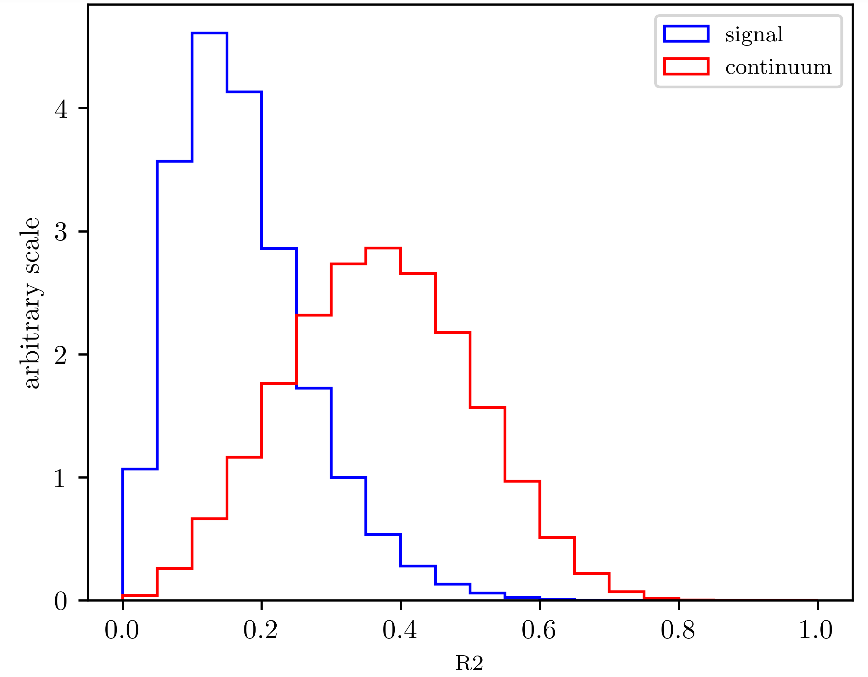
\includegraphics[width=0.75\textwidth]{04-chargedCorrBtoLambda/figs/R2EventLevel_sig_qqbar_distributions.png}}
\caption{Distribution of the $foxWolframR2$ variable for signal and continuum background events.}
\label{fig:R2distributions}
\end{figure}


\begin{figure}[h!]
%\centering
{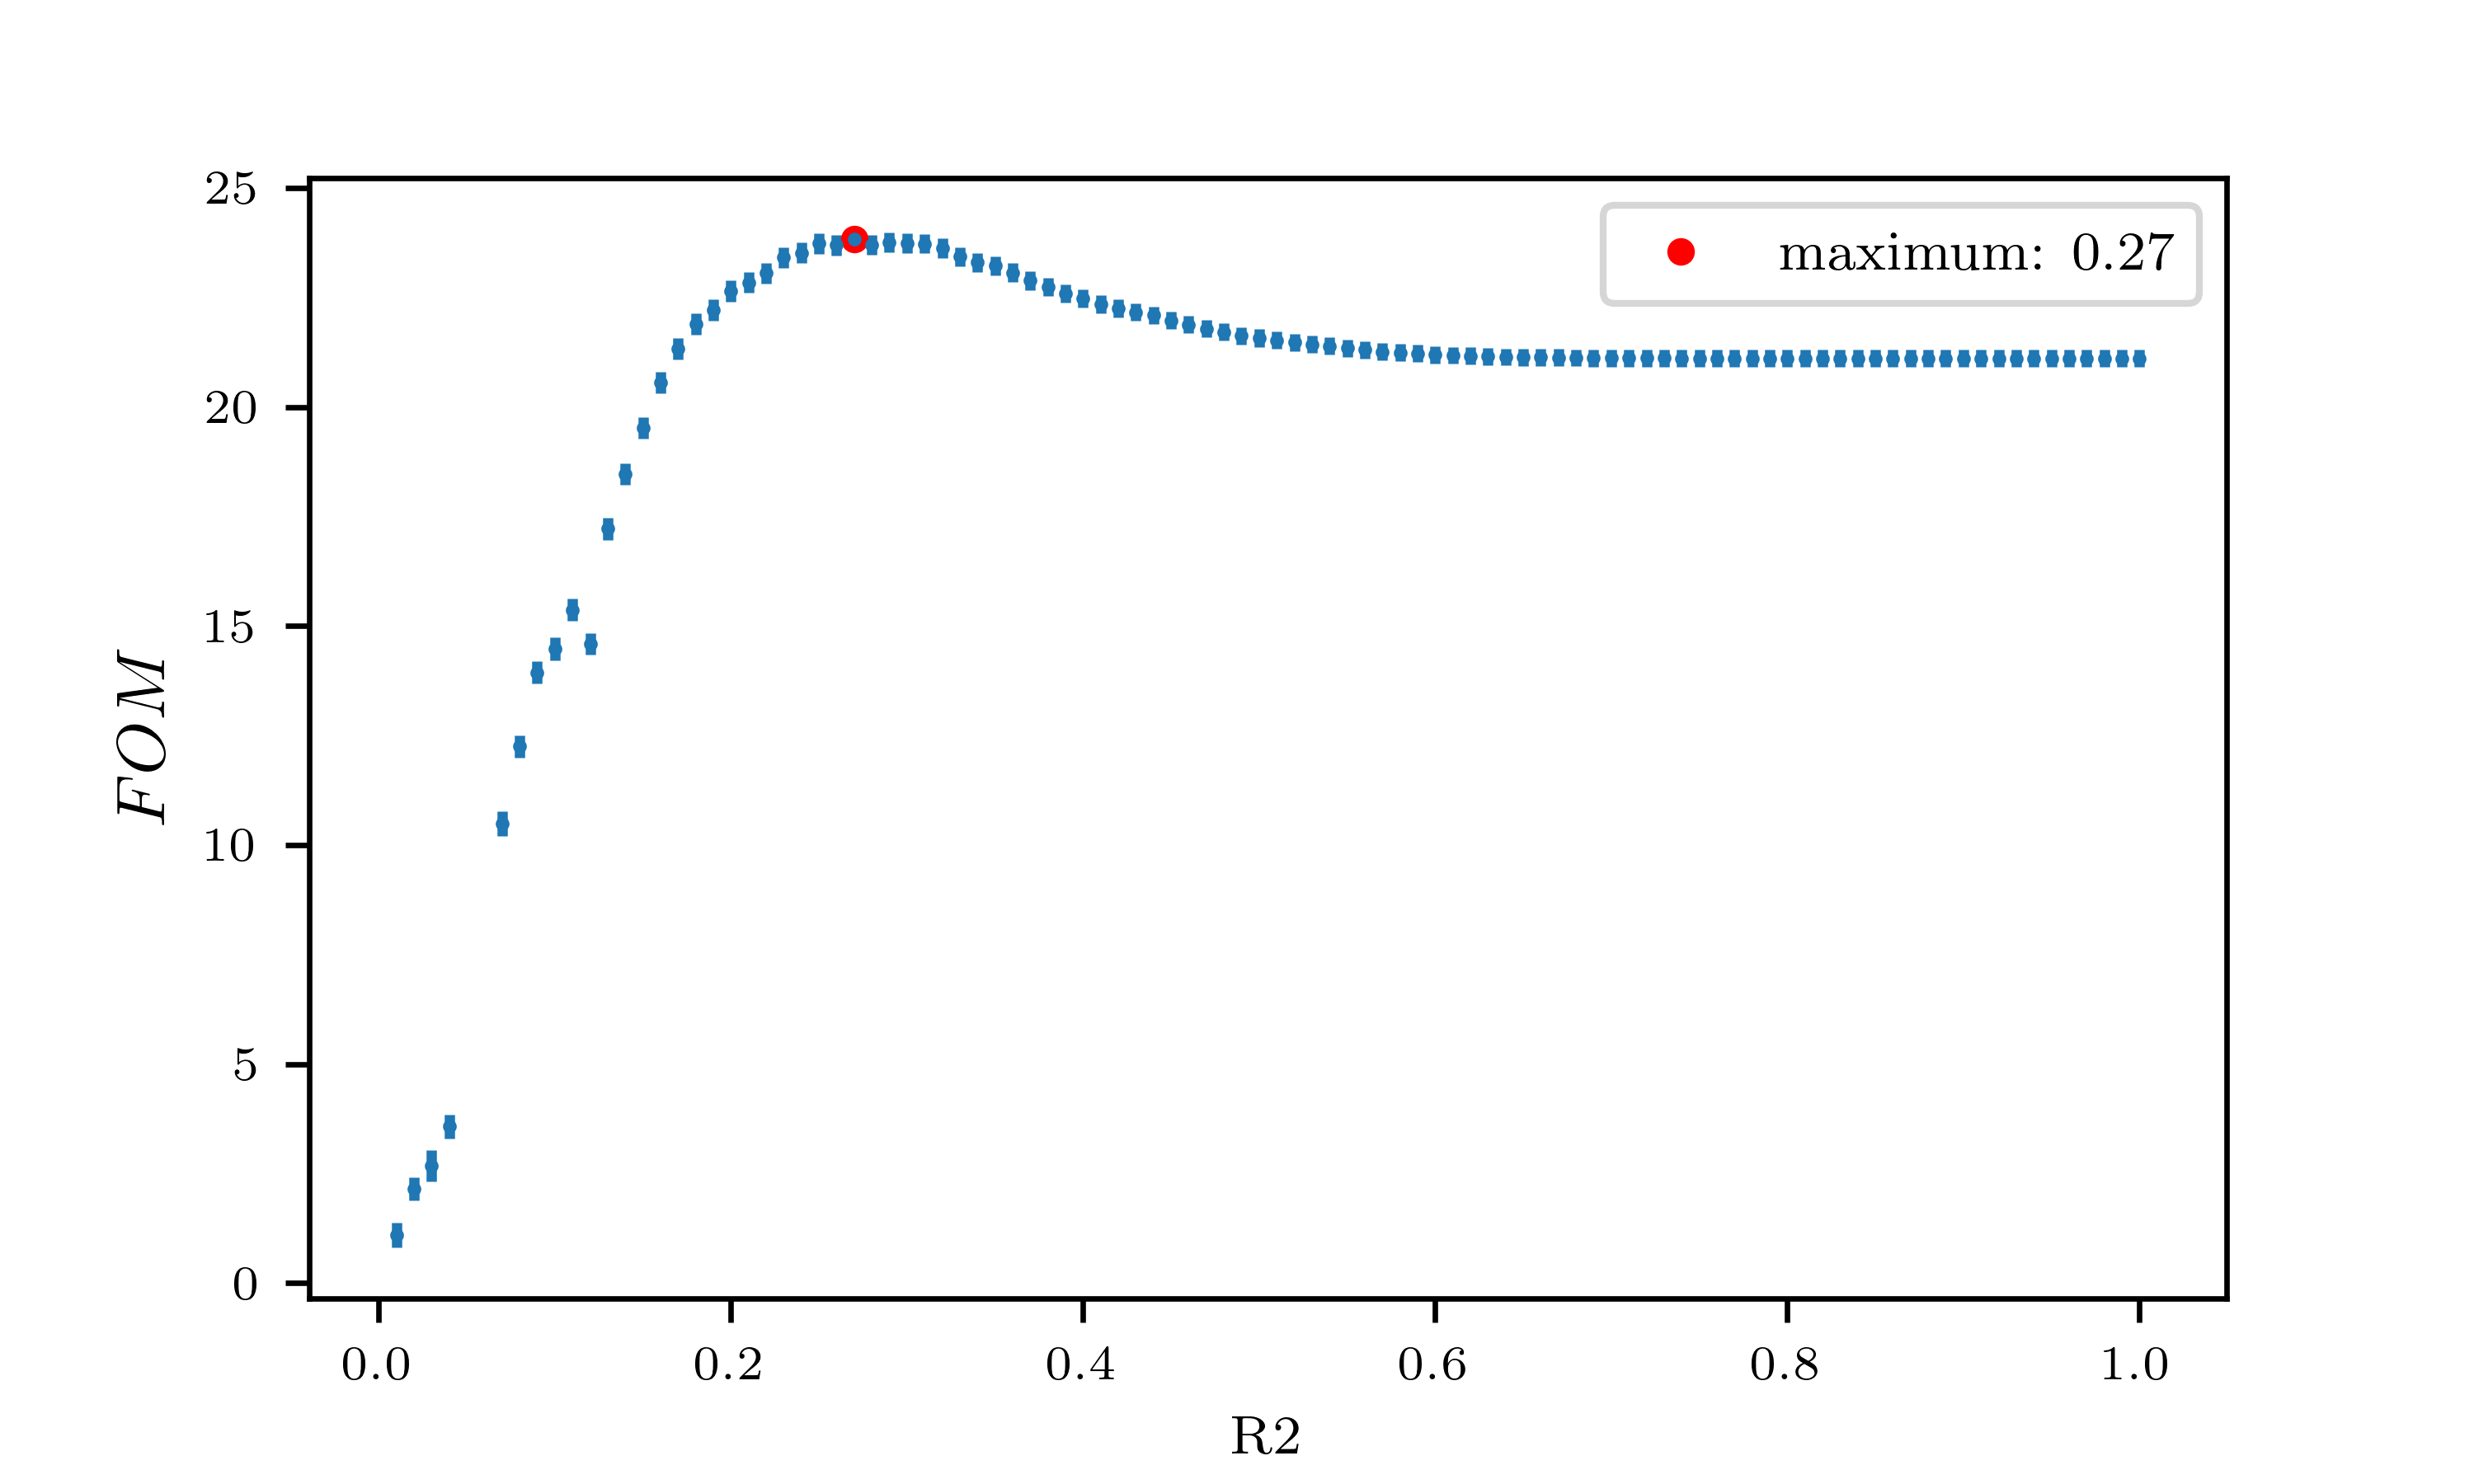
\includegraphics[width=0.75\textwidth]{04-chargedCorrBtoLambda/figs/corr_chargedB_FOMvsR2_cut.png}}
\caption{Figure of Merit values calculated at several cuts on the $foxWolframR2$ variable}
\label{fig:corr_chargedB_FOMvsR2_cut}
\end{figure}

\begin{figure}[h!]
%\centering
{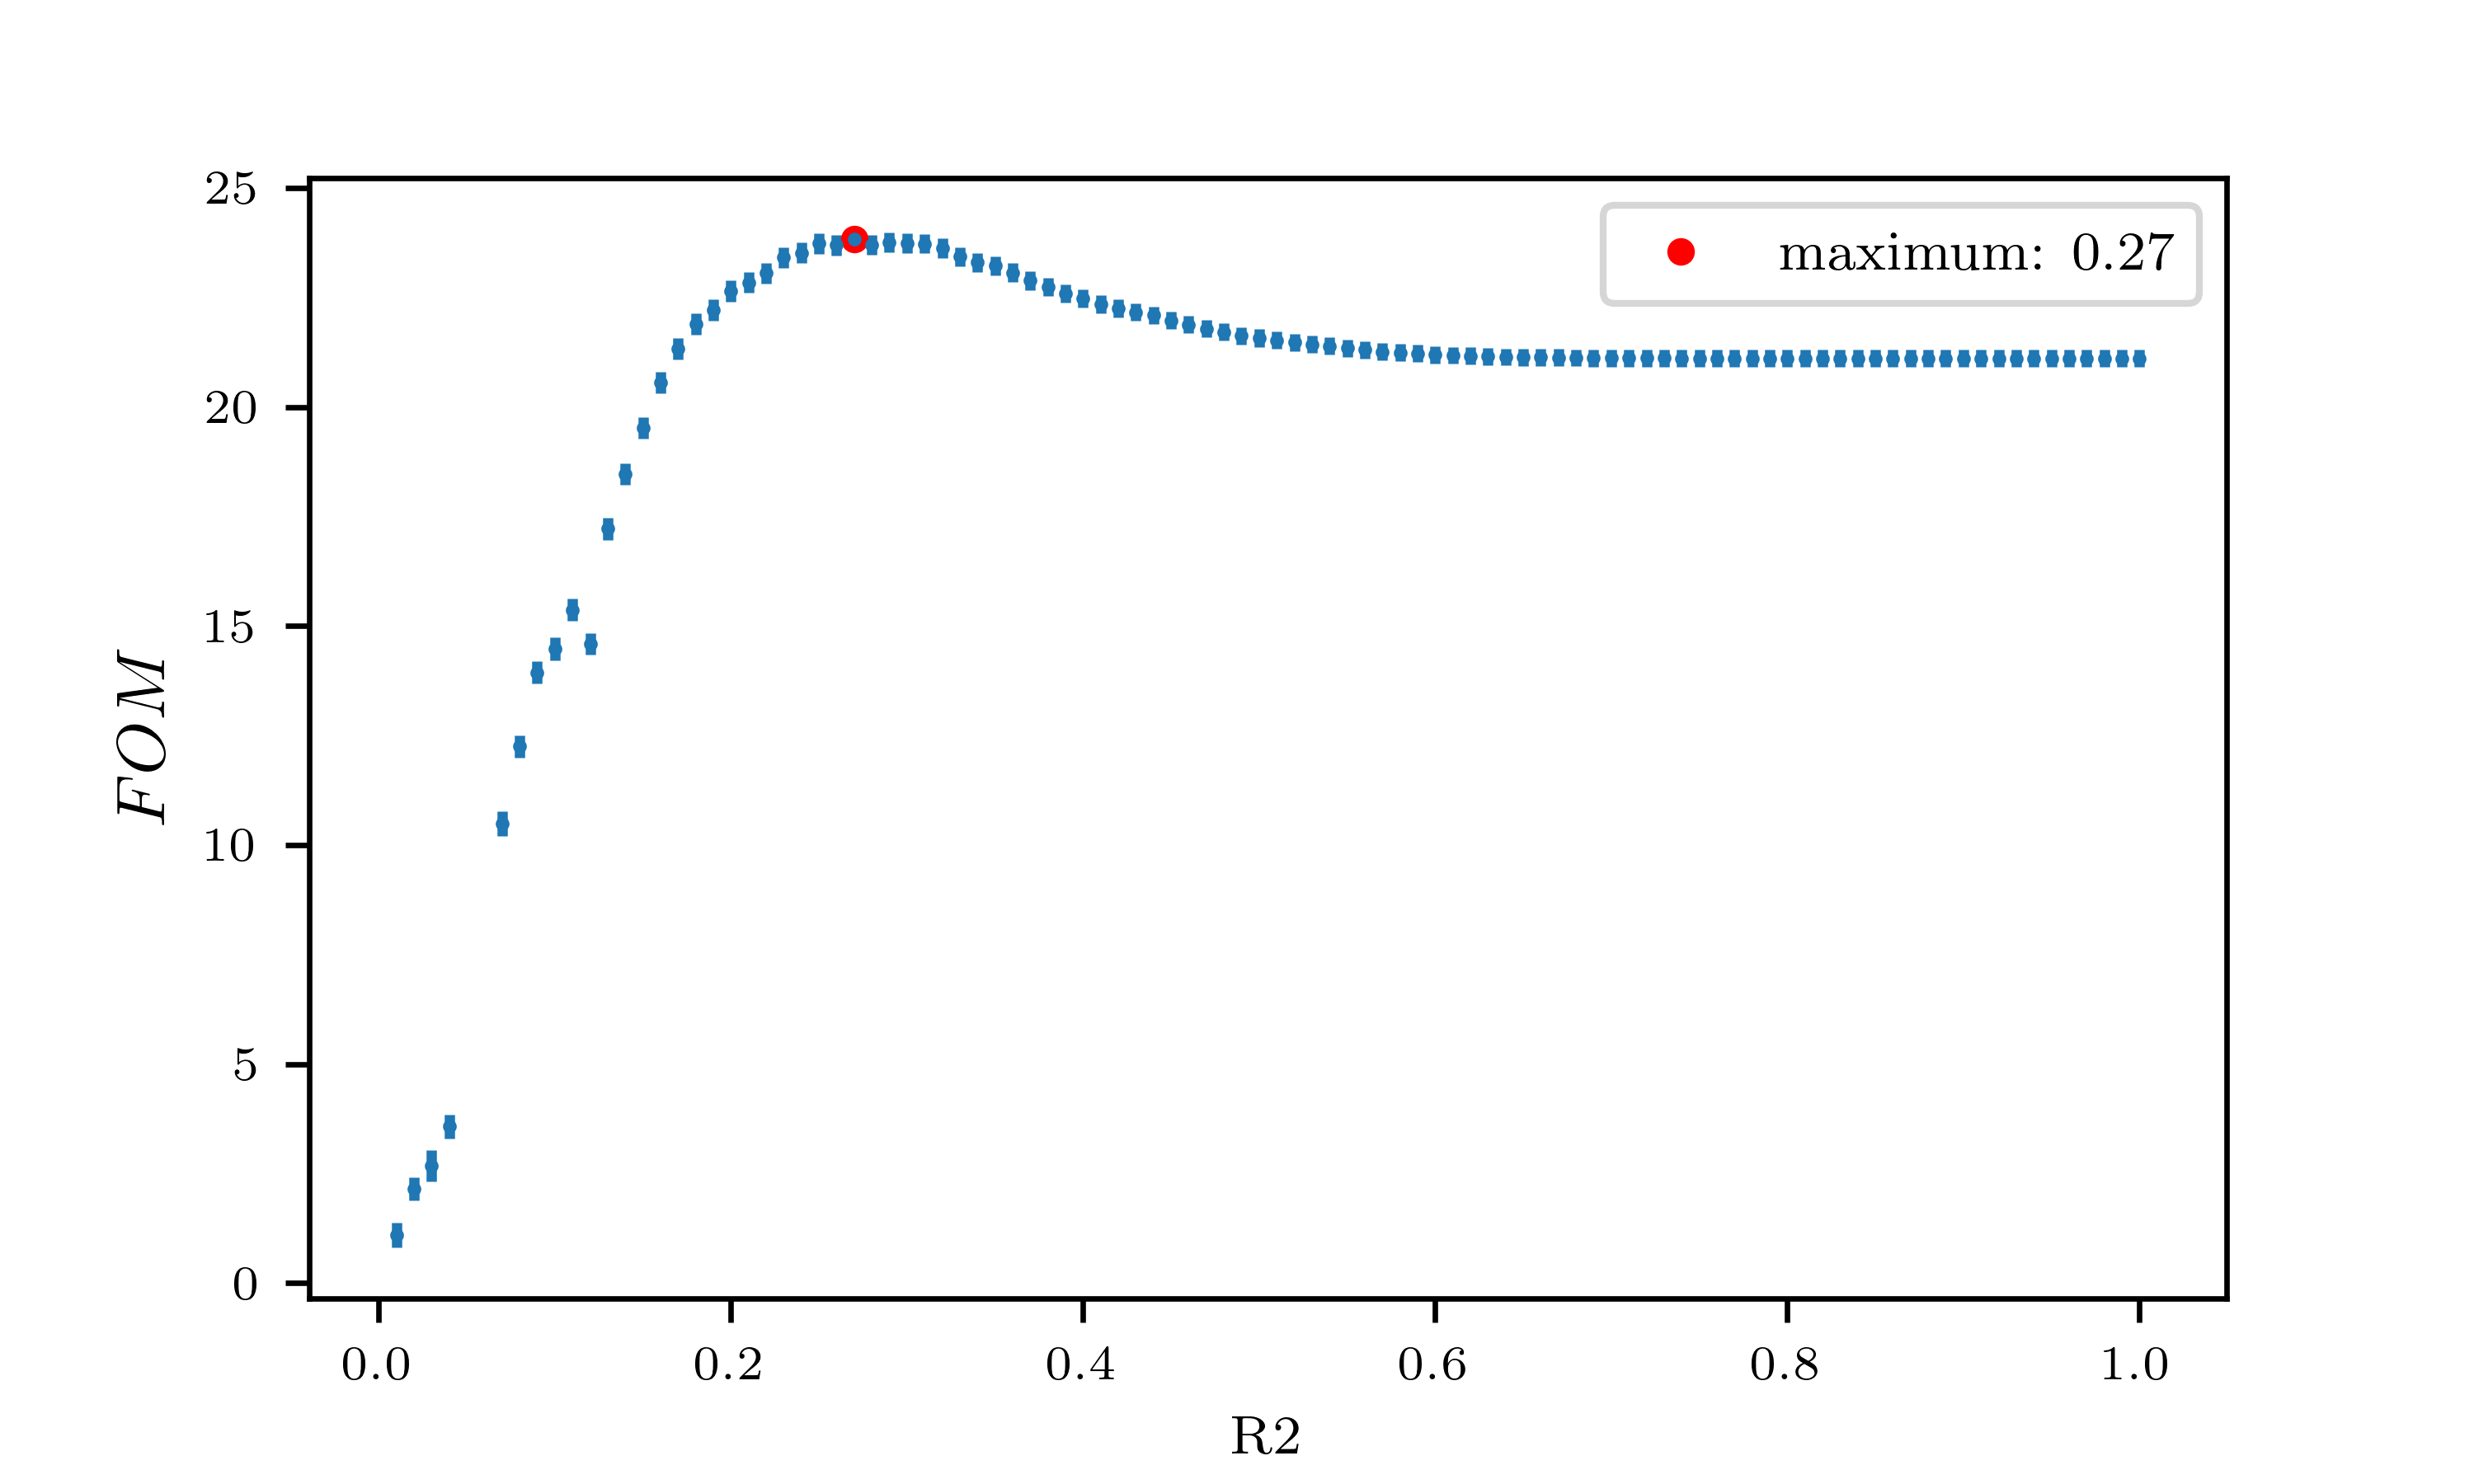
\includegraphics[width=0.75\textwidth]{04-chargedCorrBtoLambda/figs/corr_chargedB_FOMvsR2_cut.png}}
\caption{Figure of Merit values calculated at several cuts on the $foxWolframR2$ variable}
\label{fig:corr_chargedB_FOMvsR2_cut}
\end{figure}

With the optimized cut $foxWolframR2 < 0.27$ , the cut on SignalProbability is optimized in the same way (see Fig. \ref{fig:corr_chargedB_FOMvsSigProb_cut}).


\begin{figure}[h!]
%\centering
{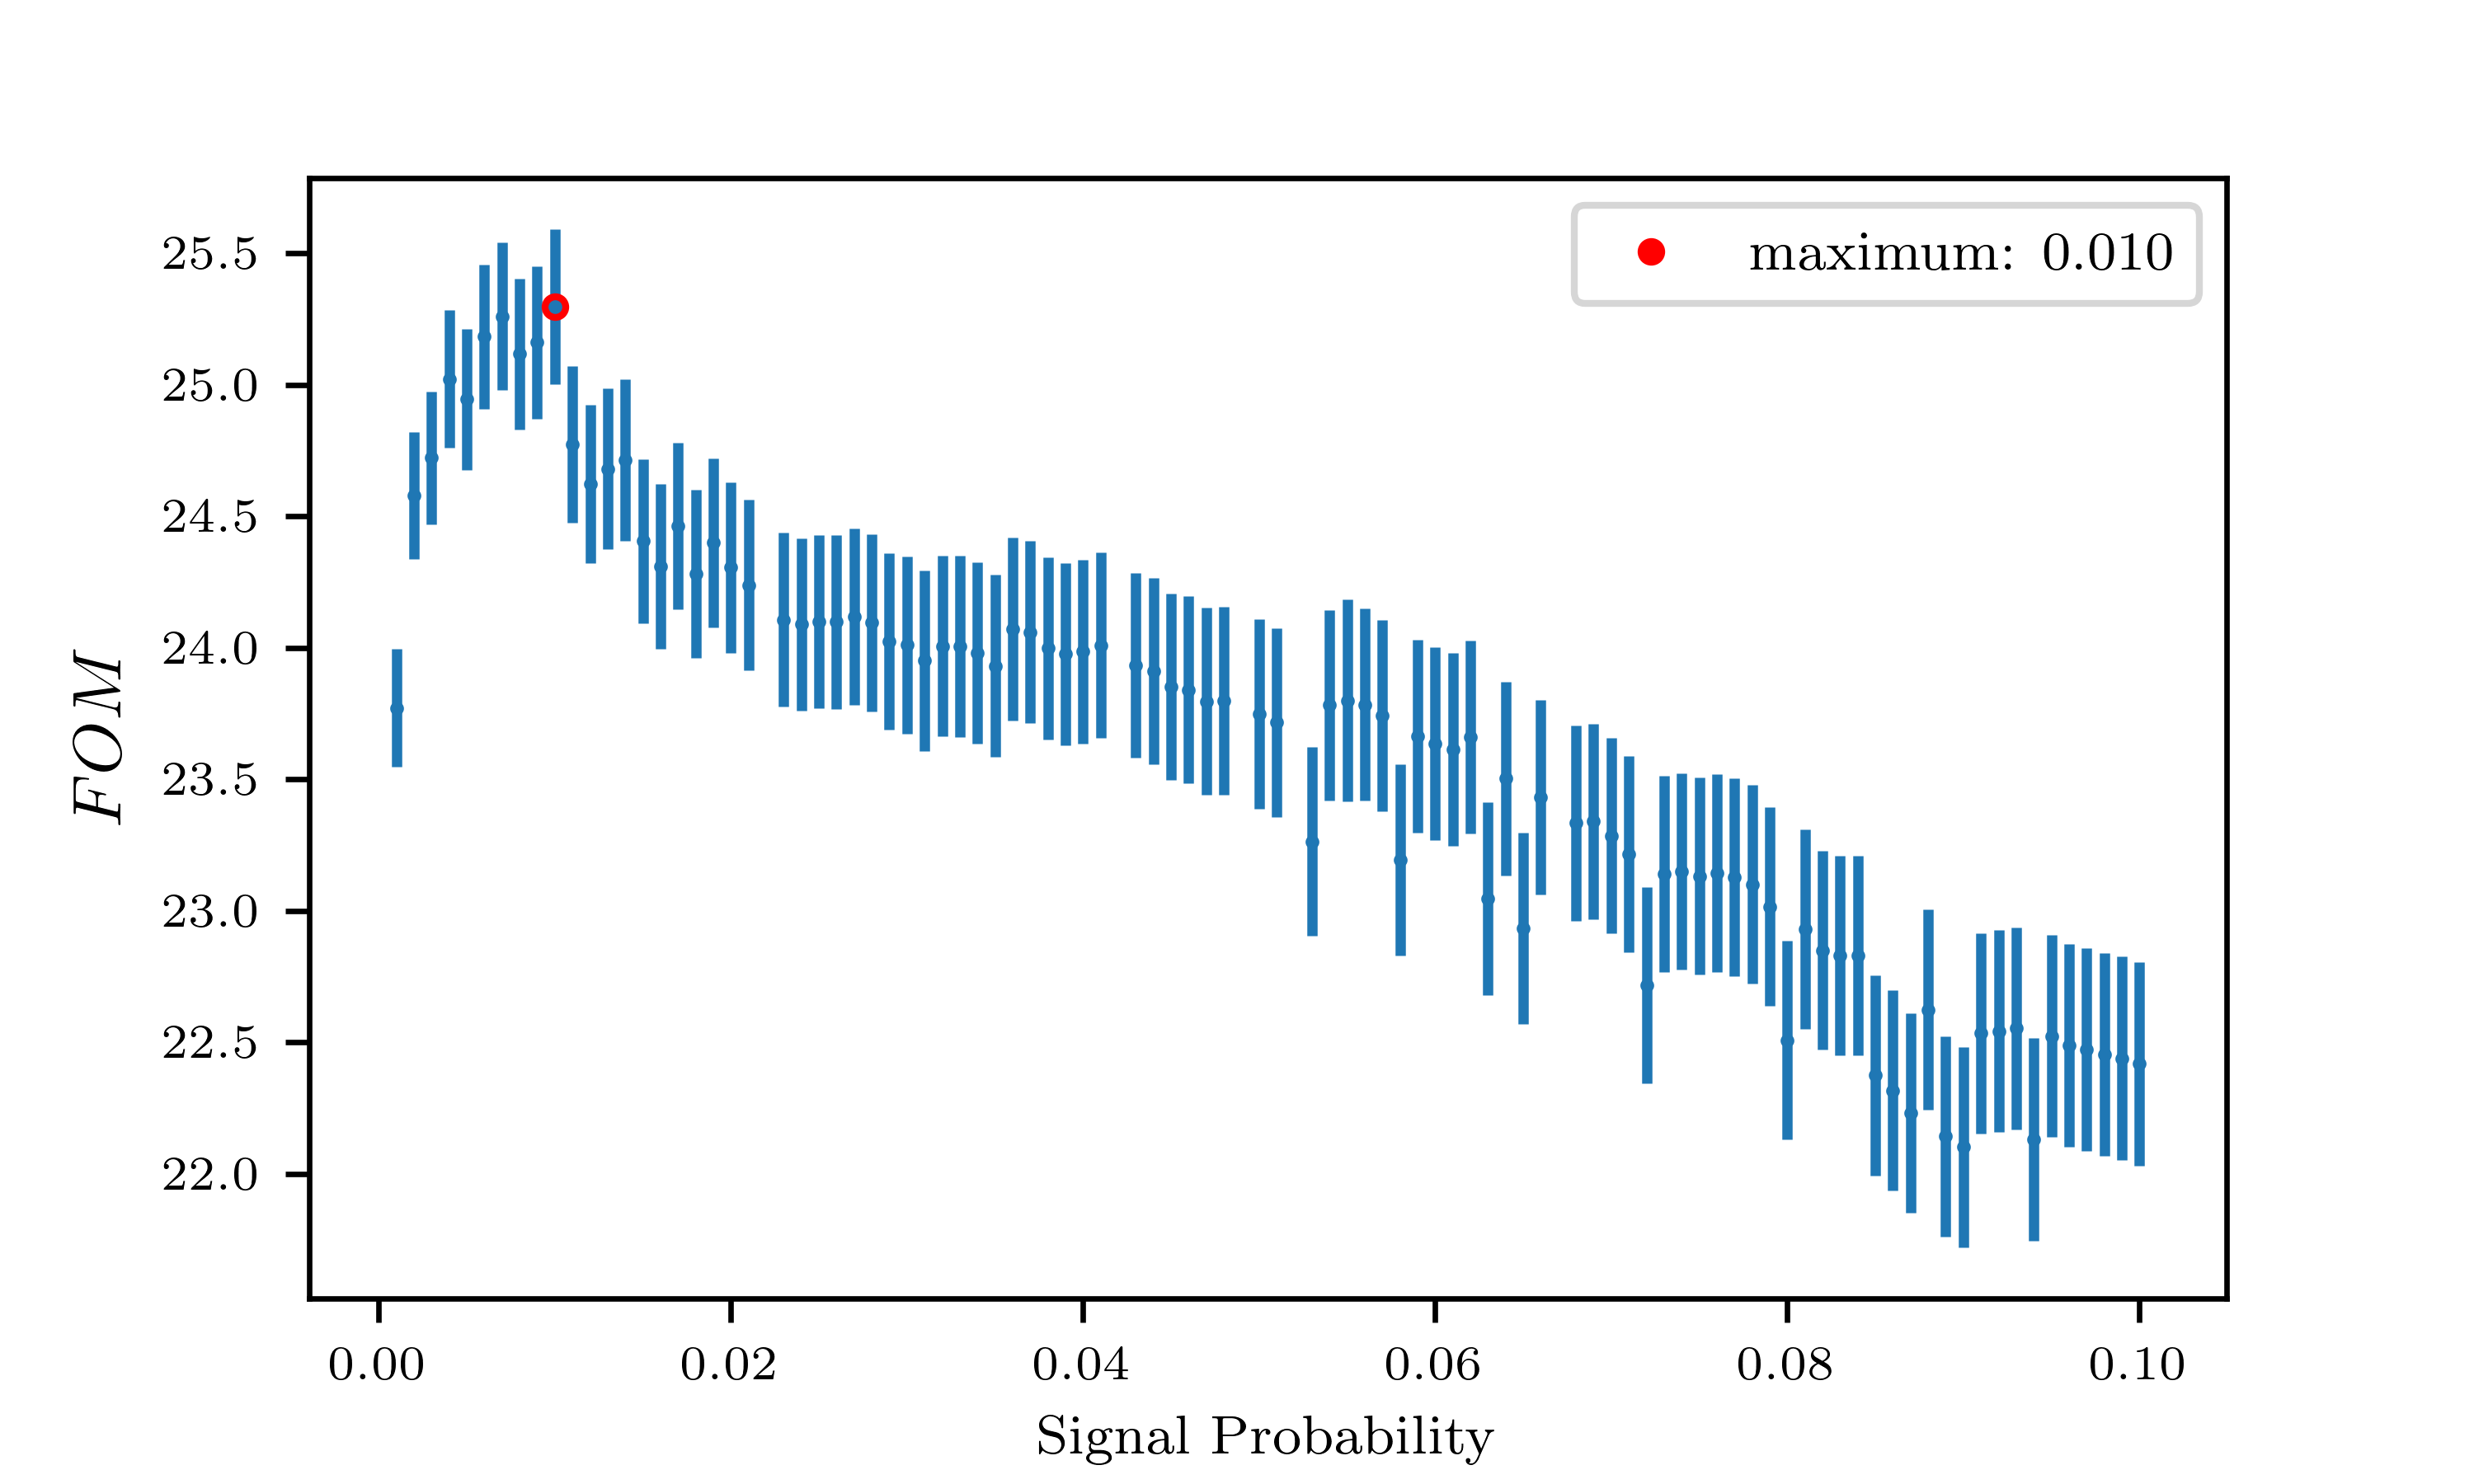
\includegraphics[width=0.75\textwidth]{04-chargedCorrBtoLambda/figs/corr_chargedB_FOMvsSigProb_cut.png}}
\caption{Figure of Merit values calculated at several cuts on the SignalProbability variable}
\label{fig:corr_chargedB_FOMvsSigProb_cut}
\end{figure}

With the optimized cut SignalProbability $ > 0.01$, the cut on $foxWolframR2$ variable is rechecked (Fig. \ref{fig:corr_chargedB_FOMvsR2_cut_SigProbOpt}). Being the maximum values fluctuating around $foxWolframR2 < 0.3$, this cut is the one finally chosen for this variable.   

\begin{figure}[h!]
%\centering
{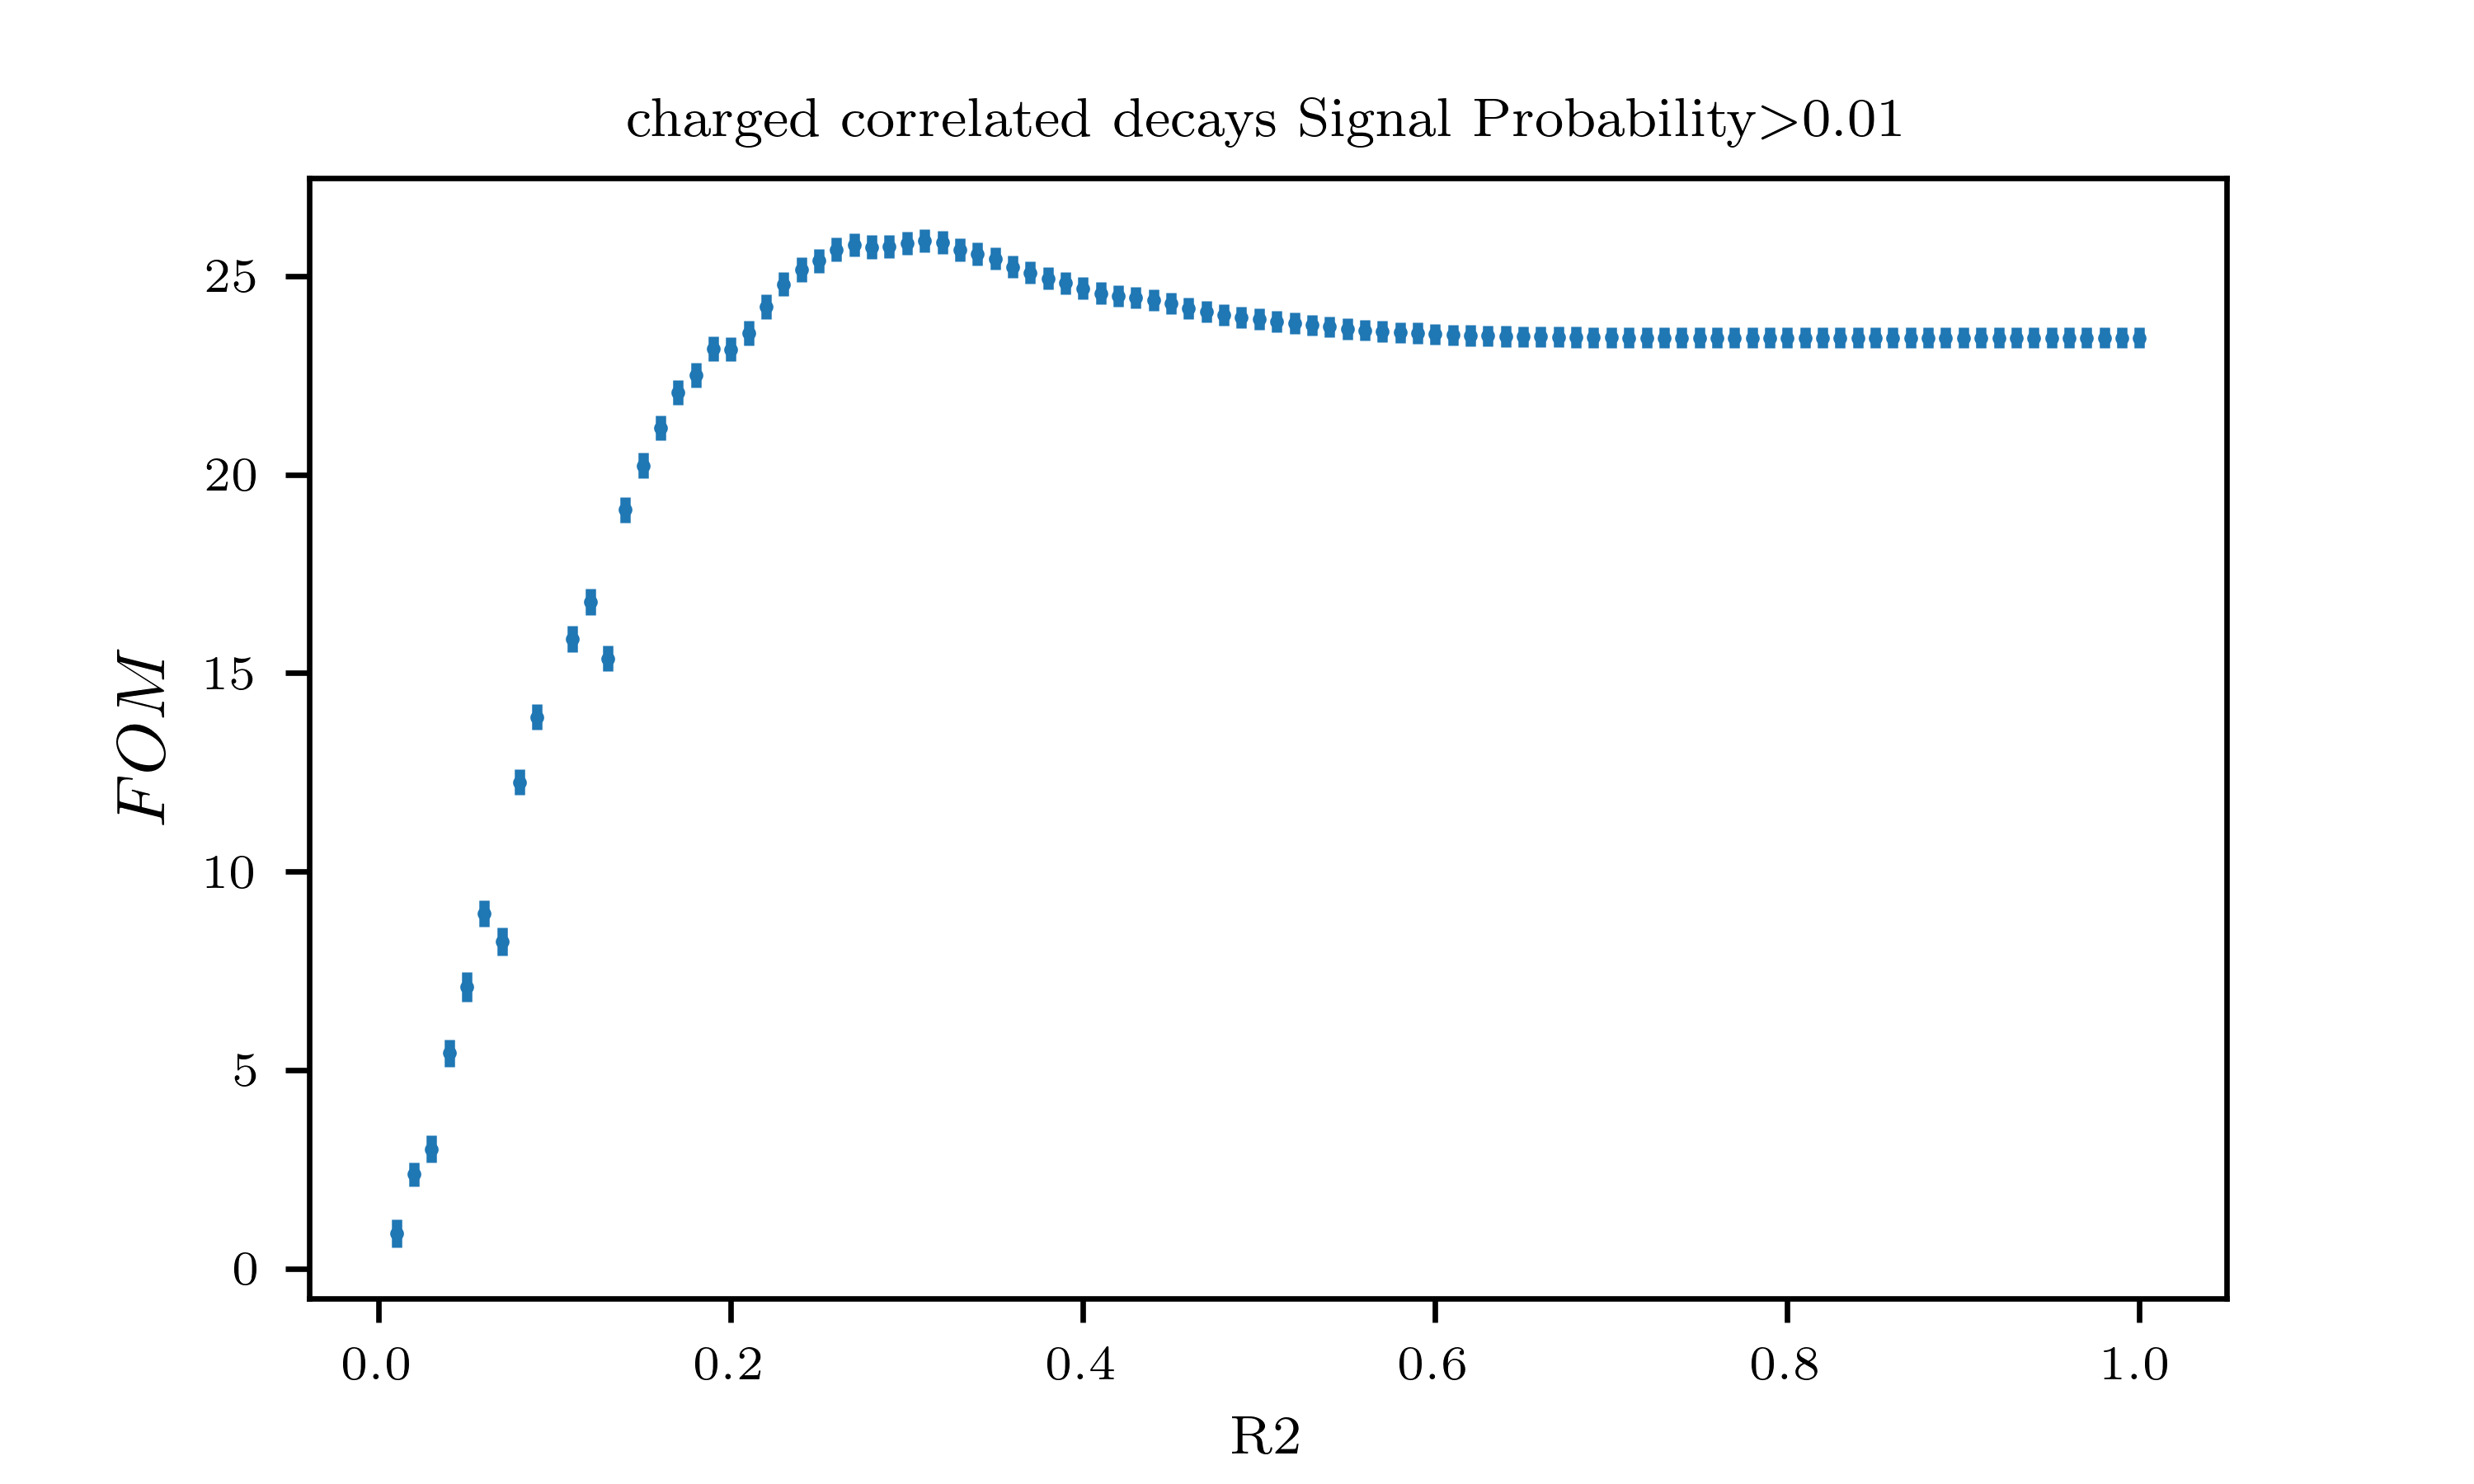
\includegraphics[width=0.75\textwidth]{04-chargedCorrBtoLambda/figs/corr_chargedB_FOMvsR2_cut_SigProbOpt.png}}
\caption{Figure of Merit values calculated at several cuts on the $foxWolframR2$ variable}
\label{fig:corr_chargedB_FOMvsR2_cut_SigProbOpt}
\end{figure}

With the optimized cuts on SignalProbability and $foxWolframR2$ variable, the cut on $p^{\Lambda_c}_{CMS}$ is optimized\\
\vspace{0.2 cm}
\newpage


\begin{figure}[h!]
%\centering
{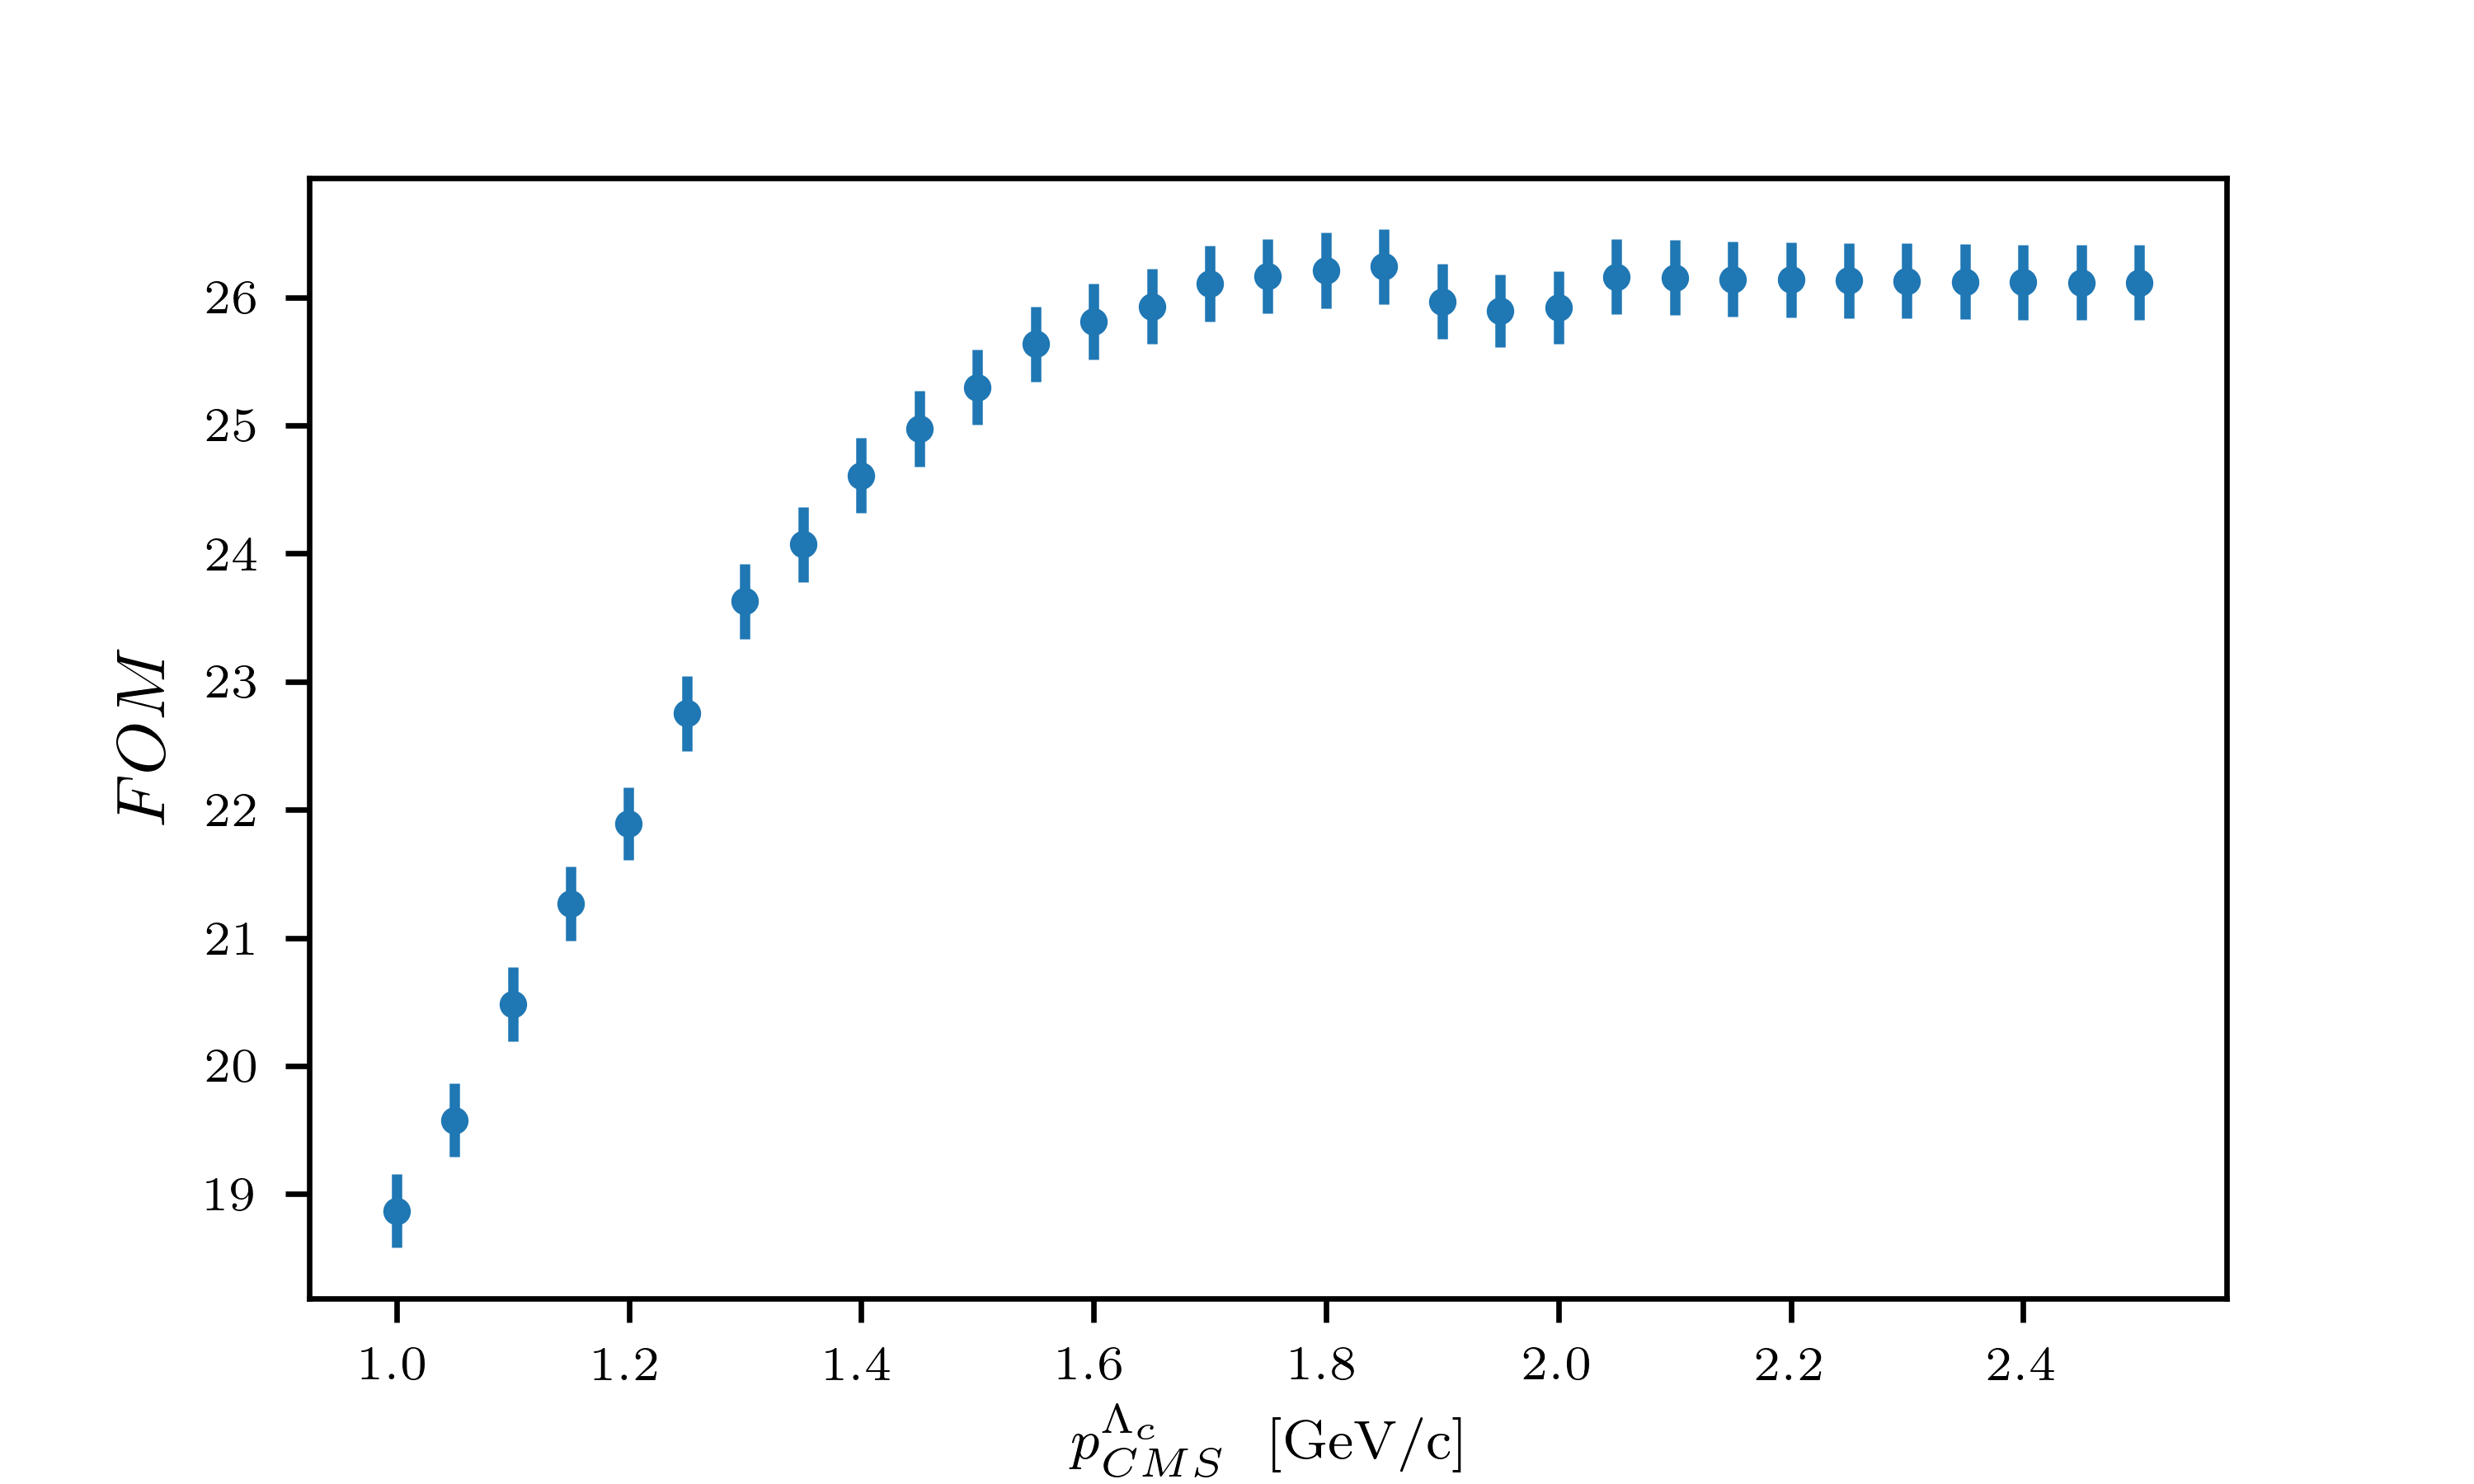
\includegraphics[width=0.85\textwidth]{04-chargedCorrBtoLambda/figs/corr_chargedB_FOMvsCMS_Pcut.png}}
\caption{Figure of Merit values calculated at several cuts on the momentum of the $\Lambda_c$ candidates in the center of mass system}
\label{fig:corr_chargedB_FOMvsCMS_Pcut}
\end{figure}
From Fig. \ref{fig:corr_chargedB_FOMvsCMS_Pcut} one can see that with values of the cut above $p^{\Lambda_c}_{CMS} <$ 1.8 GeV/$c^2$ a plateau of maximum FOM values is reached. But such a cut would still be useful to reject some background events as one can see from Fig. \ref{fig:LogPlotchargedBcorr_Lambda_c_CMS_P_optimisedSigProb_R}. 

\newpage

\begin{figure}[h!]
%\centering
{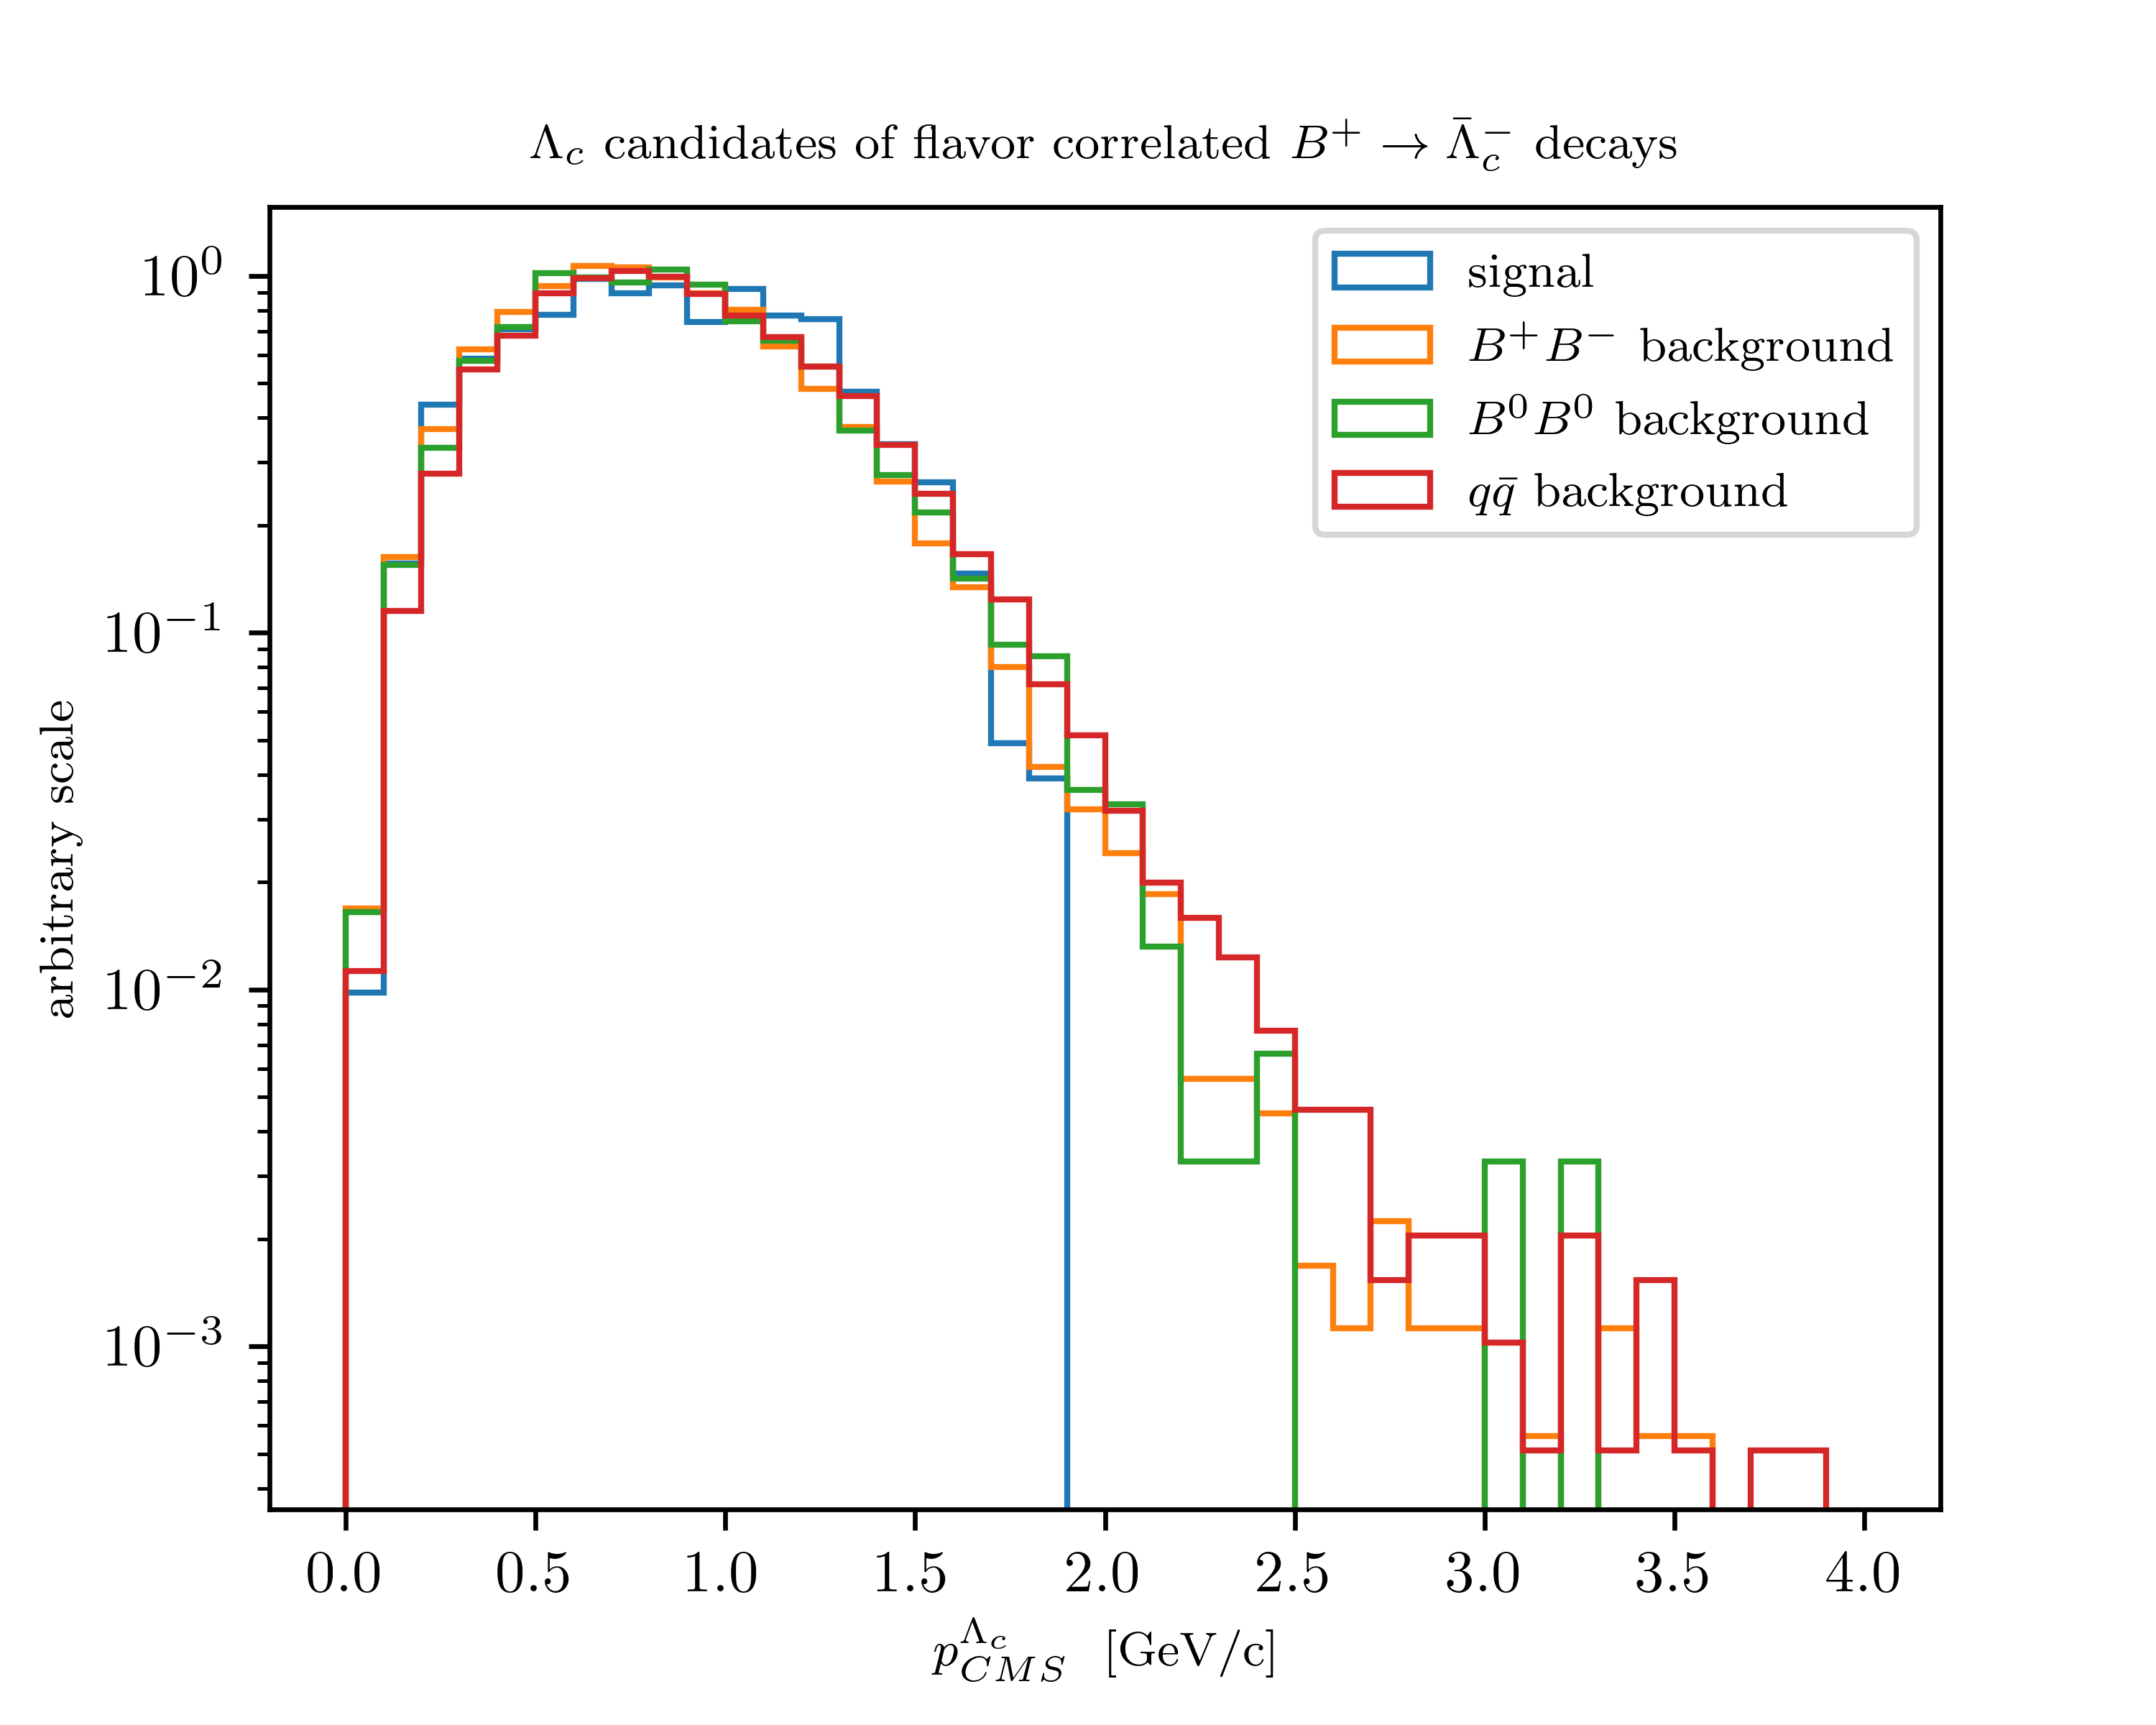
\includegraphics[width=0.85\textwidth]{04-chargedCorrBtoLambda/figs/LogPlotchargedBcorr_Lambda_c_CMS_P_optimisedSigProb_R.png}}
\caption{Distribution of  $\Lambda_c$ candidates momenta in the center of mass system}
\label{fig:LogPlotchargedBcorr_Lambda_c_CMS_P_optimisedSigProb_R}
\end{figure}

\begin{figure}[h!]
%\centering
{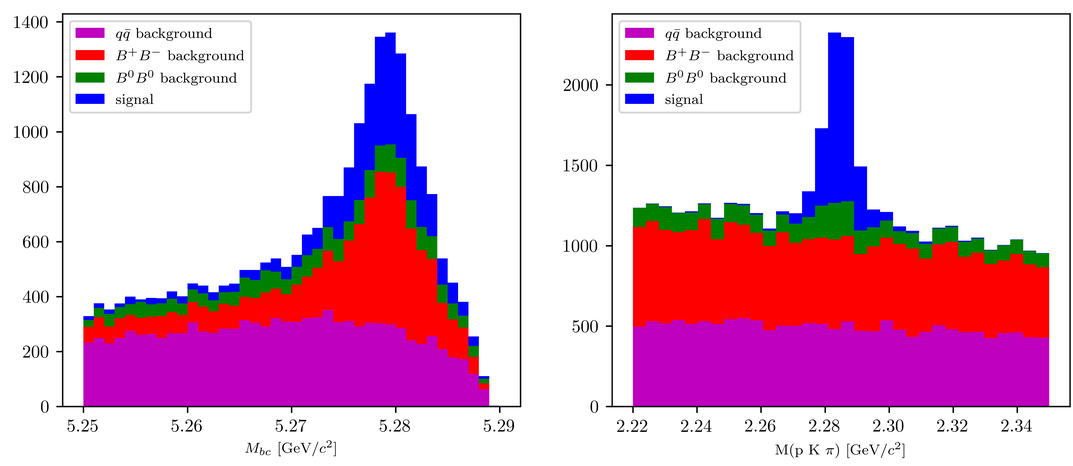
\includegraphics[width=0.95\textwidth]{04-chargedCorrBtoLambda/figs/Mbc_InvM_optimizedSelection_SigR.png}}
\caption{Distribution of $M_{bc} $ (left) and invariant mass of charged correlated $\Lambda_c$  candidates (right), in the signal region after the above mentioned selection cuts.}
\label{fig:Mbc_InvM_optimizedSelection_SigR}
\end{figure}

\mbox{
\includegraphics[width=.8\textwidth]{04-chargedCorrBtoLambda/figs/blank.png}} %
\vfill
%
%\subsection{$B^- \rightarrow \Lambda_c^-$ decays}
\vspace*{10.5cm}
.\\
%\bigskip

\mbox{~}
%\subsection{Fitting ($B^- \rightarrow \Lambda_c^+ X$ decays)}

To measure the inclusive branching fraction of $B^-  \rightarrow \Lambda_c^+ X$ the following quantities need to be known: 

\begin{equation}
    Br(B^- \rightarrow \Lambda_c^+ X) = \frac{ N_{tag, \Lambda_c} \cdot  \epsilon^{+}_{FEI}}{N_{tag} \cdot Br(\Lambda_c^+ \rightarrow  p K^- \pi^+) \epsilon_{\Lambda_c} \epsilon^{+}_{FEI,  sig }}
\end{equation}\label{eq:BRformula}

Where 
\begin{itemize}

\item $N_{tag, \Lambda_c} $ is the reconstructed signal yield obtained from a two dimensional fit of $M_{bc}$ and $M(p K \pi)$ in the final sample.
\item ${N_{tag}}$ is the reconstructed signal yield obtained from the $M_{bc}$ fit of all the tagged $B$ mesons in the final sample.
\item $\epsilon_{\Lambda_c} $ is the $\Lambda_c$ reconstruction efficiency.
\item $\epsilon^{+}_{FEI}$ represents the hadronic tag-side efficiency for generic $B^+B^- $ events. 
\item $\epsilon^{+}_{FEI,  sig}$ represents the hadronic tag-side efficiency for  $B^+B^-$ events where the tagged $B$ meson decays hadronically and the accompanying meson decays inclusively into the studied signal channel. 
\item  $Br(\Lambda_c^+ \rightarrow  p K^- \pi^+) $: the branching fraction of the decay mode used to reconstruct the  $\Lambda_c$ baryon.
\end{itemize}
\vspace{0.2 cm}
Here a decision was made not to rely on the estimated number of $B$ meson pair, as it is usually done, and the absolute FEI efficiency, since the latter shows large discrepancy between MC and data (see i.e. the results reported in the PhD Thesis by M. Gelb \cite{gelb_moritz_2018_21546} and also by J. Schwab \cite{schwab_judith_2017_21422} ) and also it depends strongly on the signal-side (i.e. $\epsilon^{+}_{FEI} \neq \epsilon^{+}_{FEI,  sig}$). Instead, to limit the systematics, the branching ratio normalization is obtained using the fitted tagged $B$ mesons and the ratio $\epsilon^{+}_{FEI,  sig} / \epsilon^{+}_{FEI}$ measured on MC, which is expected to be described much better rather than the absolute FEI efficiency.  

The final samples contain both signal and background candidates
from various sources and in order to extract $N_{tag, \Lambda_c} $ and ${N_{tag}}$  unbinned extended maximum-likelihood fits are performed.  \\
In the next sections the methods used to determine the above mentioned quantities are described. First the fit model that accurately describes the   distributions in the $B_{tag}+\Lambda_c$ final sample will be described.

\vspace{0.5 cm}

\subsection{Probability Density Functions (PDFs) for the two dimensional fit}\label{sec:2DpdfChargedCorrBtoLambdaC}

The PDFs used to describe the signal distributions are discussed first. The final sample of total signal events presents a peak around the expected $B$ meson mass and a tail at low $M_{bc}$ values. 
\begin{figure}[H]
%\centering
{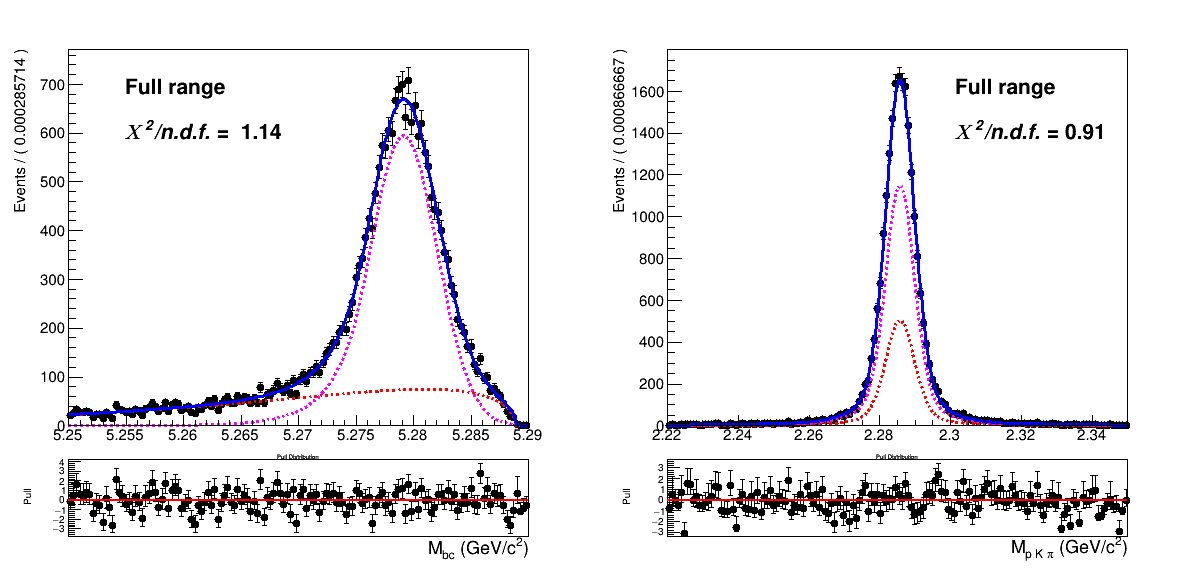
\includegraphics[width=0.9\textwidth]{04-chargedCorrBtoLambda/figs/5streams_TotalSignal_charged_corrLambdaC_2Dfit.png}}
\caption{Two dimensional fit of total signal events in $M_{bc}$  and $M(p K \pi)$ }
\label{fig:5streams_TotalSignal_charged_corrLambdaC_2Dfit}
\end{figure}

The 2D fit shown in Fig. \ref{fig:5streams_TotalSignal_charged_corrLambdaC_2Dfit} is performed on five streams of signal MC with a sum of the following probability density functions:
\vspace{0.2 cm}
 \begin{equation}
        P^{recSig}_{B,\Lambda_c}(M_{bc}, M(p K \pi)) = \Gamma_{CB}(M_{bc}) \times \rho_G(M(p K \pi))
    \label{eq:RecSigEq}
\end{equation} 
\begin{equation}
        P^{misSig}_{B,\Lambda_c}(M_{bc}, M(p K \pi)) = \Gamma_{ARG}(M_{bc}) \times \rho_G(M(p K \pi))
    \end{equation}  \label{eq:MisSigEq}

The first is used to fit the reconstructed signal and $\Gamma_{CB}(M_{bc})$ is a Crystal Ball function. The second is used to model the misreconstructed signal and $\Gamma_{ARG}(M_{bc})$ is an Argus function. In both cases a sum of three Gaussian functions $\rho_G(M(p K \pi))$ describes the mass of the $\Lambda_c$ baryon.  


%\newpage
As already said in Sec. \ref{wronglyBtag}, only the reconstructed signal considered for the signal yield, while the misreconstructed signal is considered as background.
Other background components that will be discussed in the next pages are:

\begin{itemize}
    \item \textbf{generic} (charged $B$) background
    \item \textbf{crossfeed} (neutral $B$) background 
    \item \textbf{continuum} background 
\end{itemize}
\vspace{0.2 cm}

\newpage
\noindent \textbf{Generic background}
\begin{figure}[H]
%\centering
{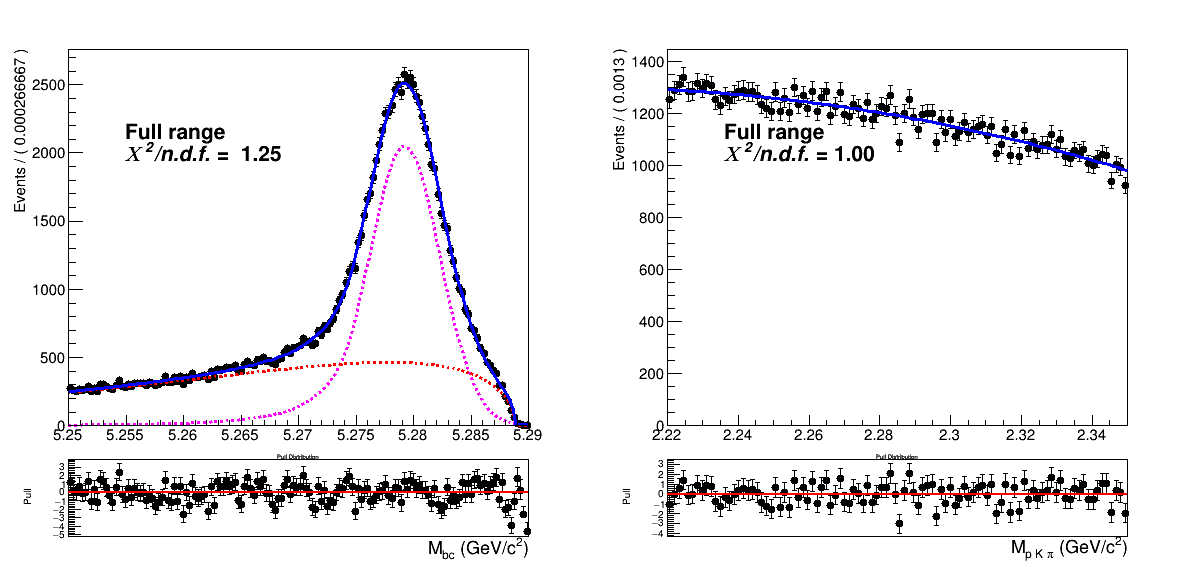
\includegraphics[width=0.9\textwidth]{04-chargedCorrBtoLambda/figs/streams12345_charged_corrLambdaC_Generic_2DFit.png}}
\caption{Two dimensional fit of generic ($B^+B^-$) events in $M_{bc}$  and $M(p K \pi)$. }
\label{fig:5streams_Generic_charged_corrLambdaC_2Dfit}
\end{figure}
\noindent The generic background deriving from other $B^{+}B^-$ events presents a 
similar shape of the distribution in $M_{bc}$ (see Fig. \ref{fig:5streams_Generic_charged_corrLambdaC_2Dfit}): the probability
density functions used for it are again a  Crystal Ball and an Argus. For both functions the parameters differ from the ones used in Eq. \ref{eq:RecSigEq}-\ref{eq:MisSigEq}.
Instead, the flat background in $M(p K \pi)$ can be described with a second order Chebychev polynomial function. The two dimensional PDF in this case is given by:

\begin{equation}
P^{GenBkg}_{B,\Lambda_c}(M_{bc}, M(p K \pi)) = [\Gamma_{CB}(M_{bc}) + \Gamma_{ARG}(M_{bc})] \times \rho_{Cheb2}(M(p K \pi))
 \end{equation}


\newpage

\noindent \textbf{Crossfeed background}
\newline
The contamination of misreconstructed $B^0$ events in the $B^+$ signal (and vice-versa) induces a background which peaks near the $B$ meson mass, as one can see in Fig. \ref{fig:chargedBcorr_Crossfeed}, indipendently from the category of events in the $\Lambda_c$ mass (see Figures \ref{fig:chargedBcorr_CrossfeedLambdaCpeak}- \ref{fig:chargedBcorr_CrossfeedNoLambdaCpeak}). 
Since among the misreconstructed $B^0$ events there are also $B^0 \rightarrow \Lambda_c $ decays (peaking at the $\Lambda_c$ mass, see e.g. \cref{fig:chargedBcorr_CrossfeedLambdaCpeak}), this background contribution is also named "crossfeed background". 

\begin{figure}[H]
\centering
{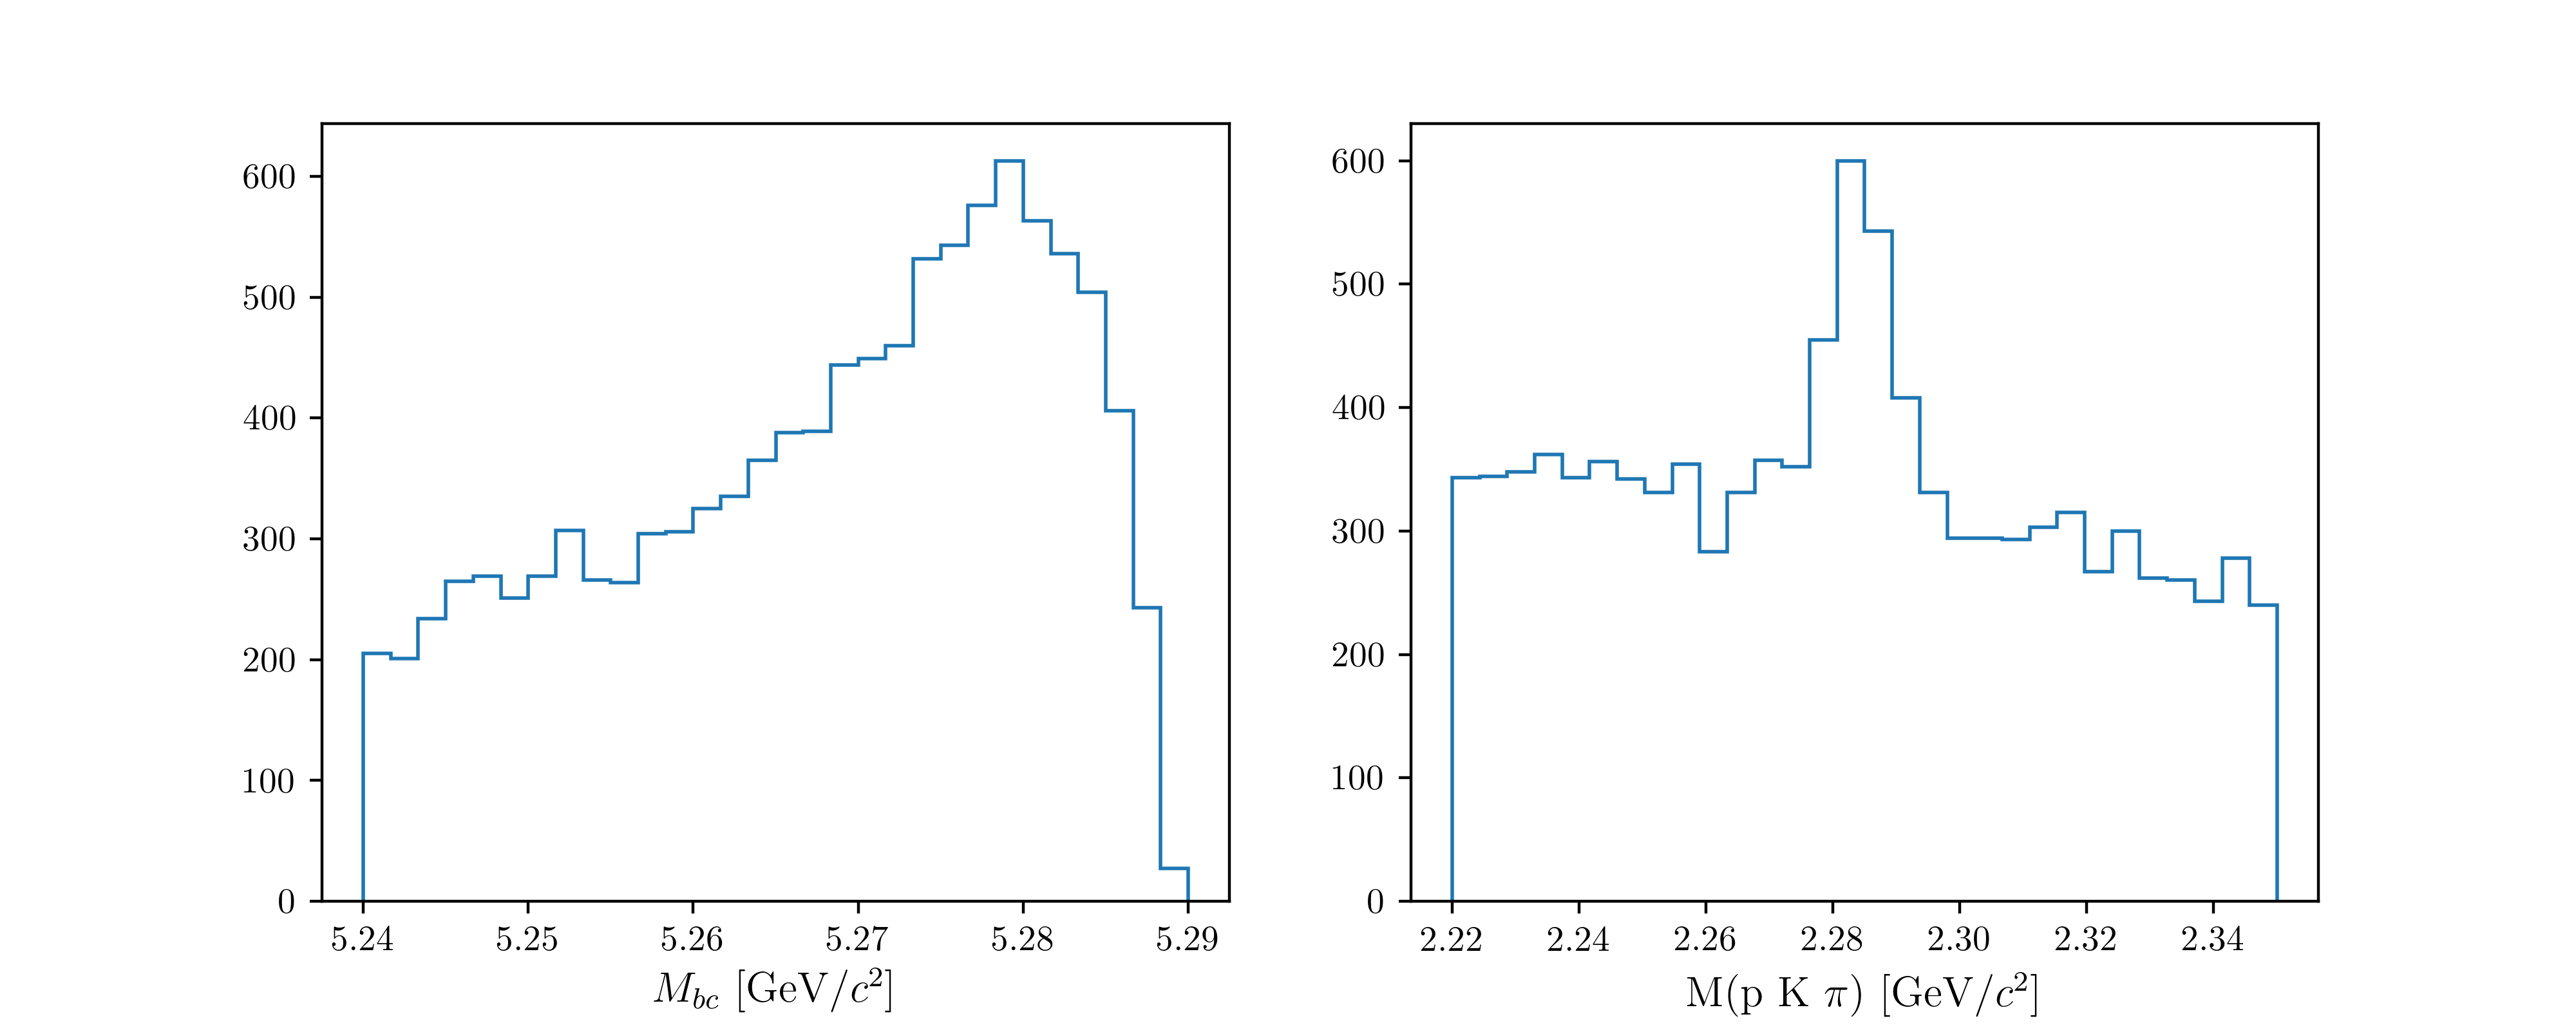
\includegraphics[width=1\textwidth]{04-chargedCorrBtoLambda/figs/chargedBcorr_Crossfeed.png}}
\caption{$M_{bc}$ and $M(p K \pi)$ distributions of crossfeed background events. }
\label{fig:chargedBcorr_Crossfeed}
\end{figure}

\begin{figure}[H]
\centering
{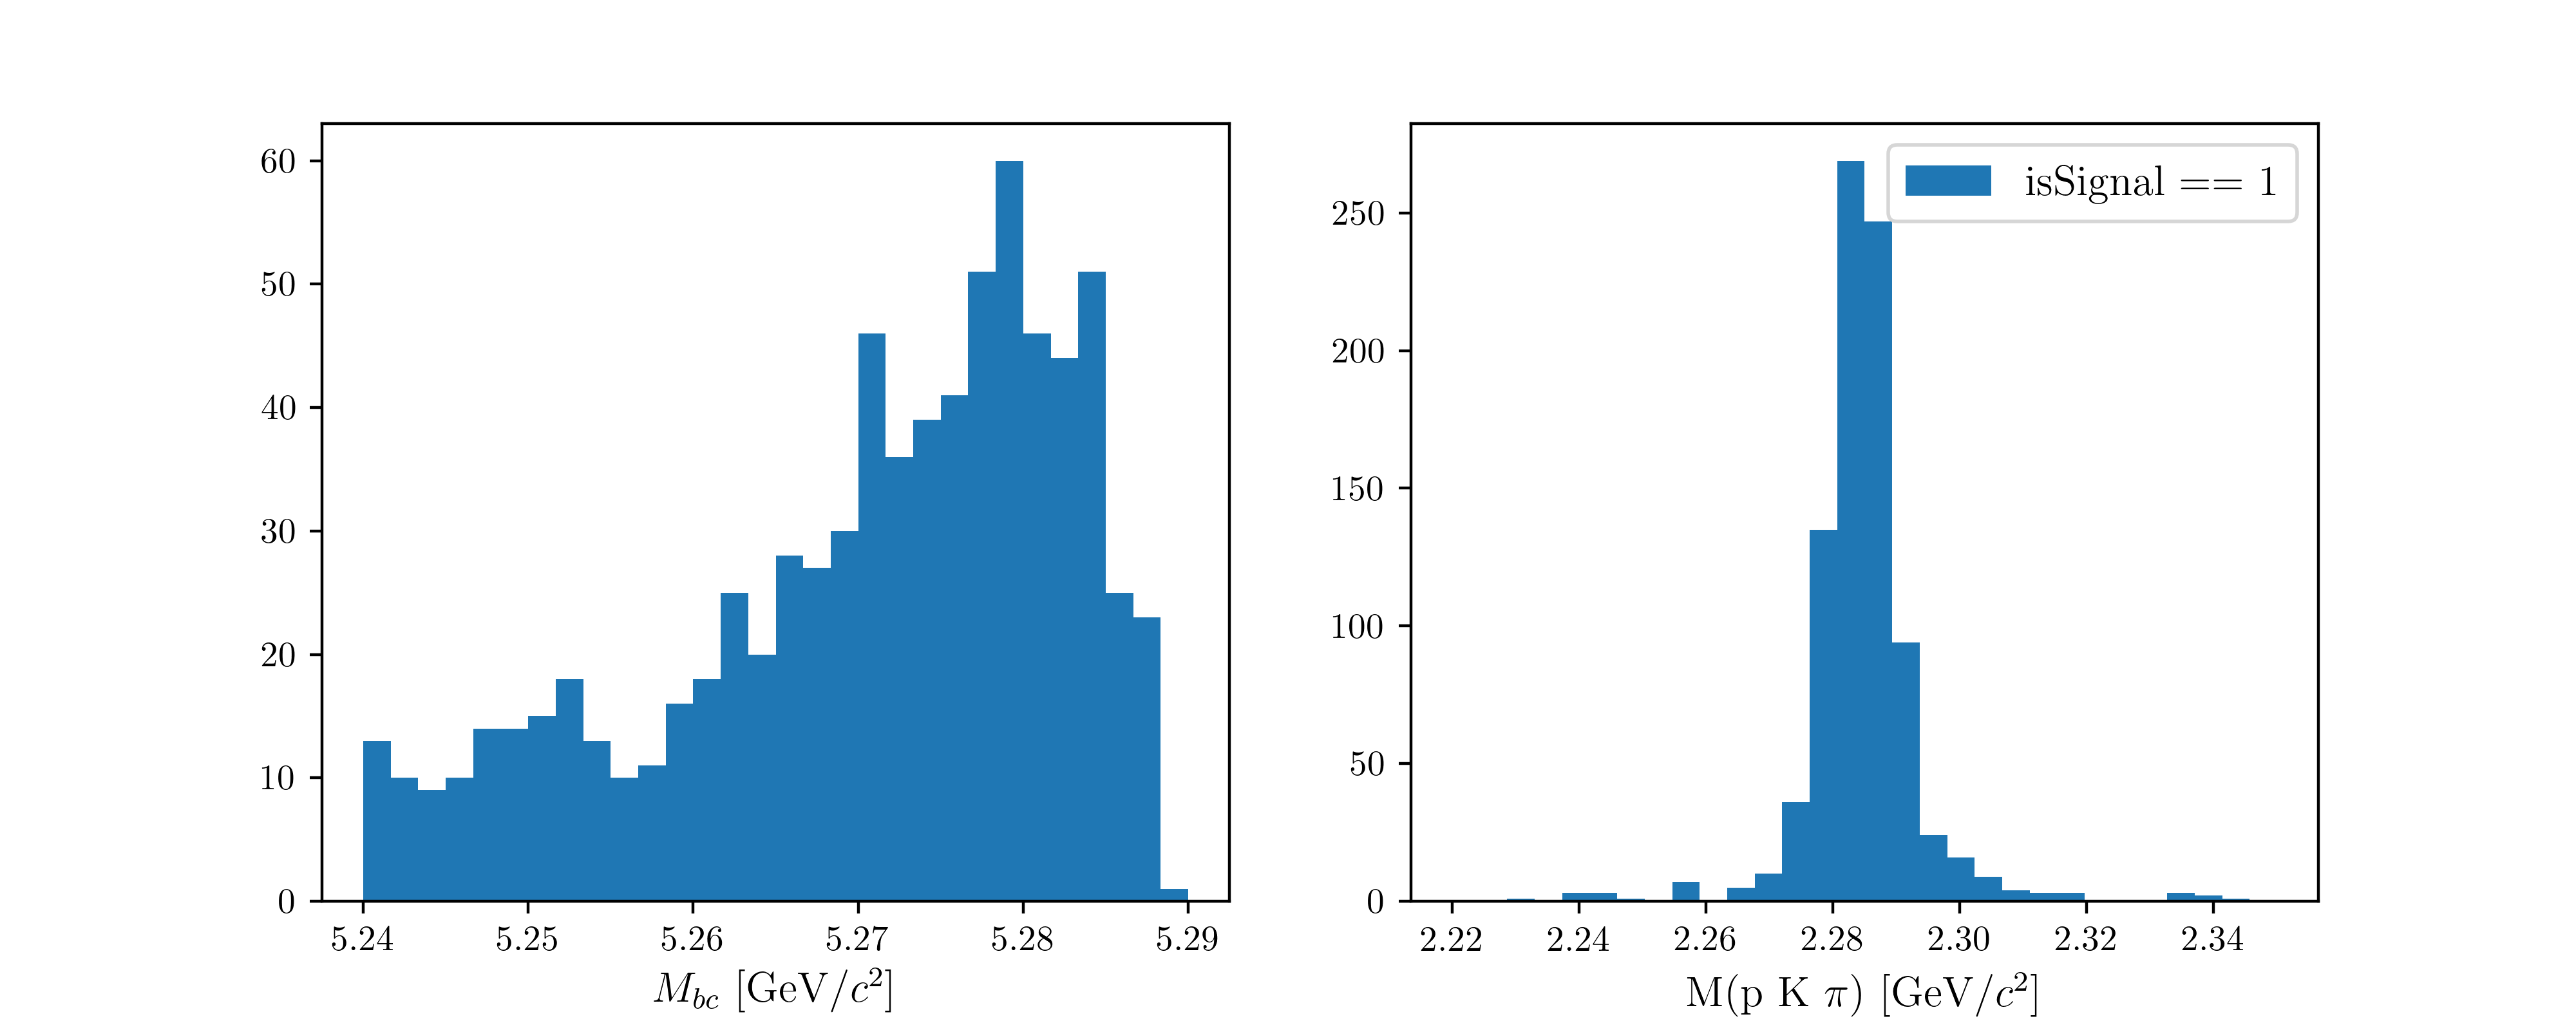
\includegraphics[width=1\textwidth]{04-chargedCorrBtoLambda/figs/chargedBcorr_CrossfeedLambdaCpeak.png}}
\caption{$M_{bc}$ and $M(p K \pi)$ of crossfeed events peaking at the $ \Lambda_c$ mass, i.e.: where true $ \Lambda_c$ baryons were correctly reconstructed. }
\label{fig:chargedBcorr_CrossfeedLambdaCpeak}
\end{figure}


\begin{figure}[H]
\centering
{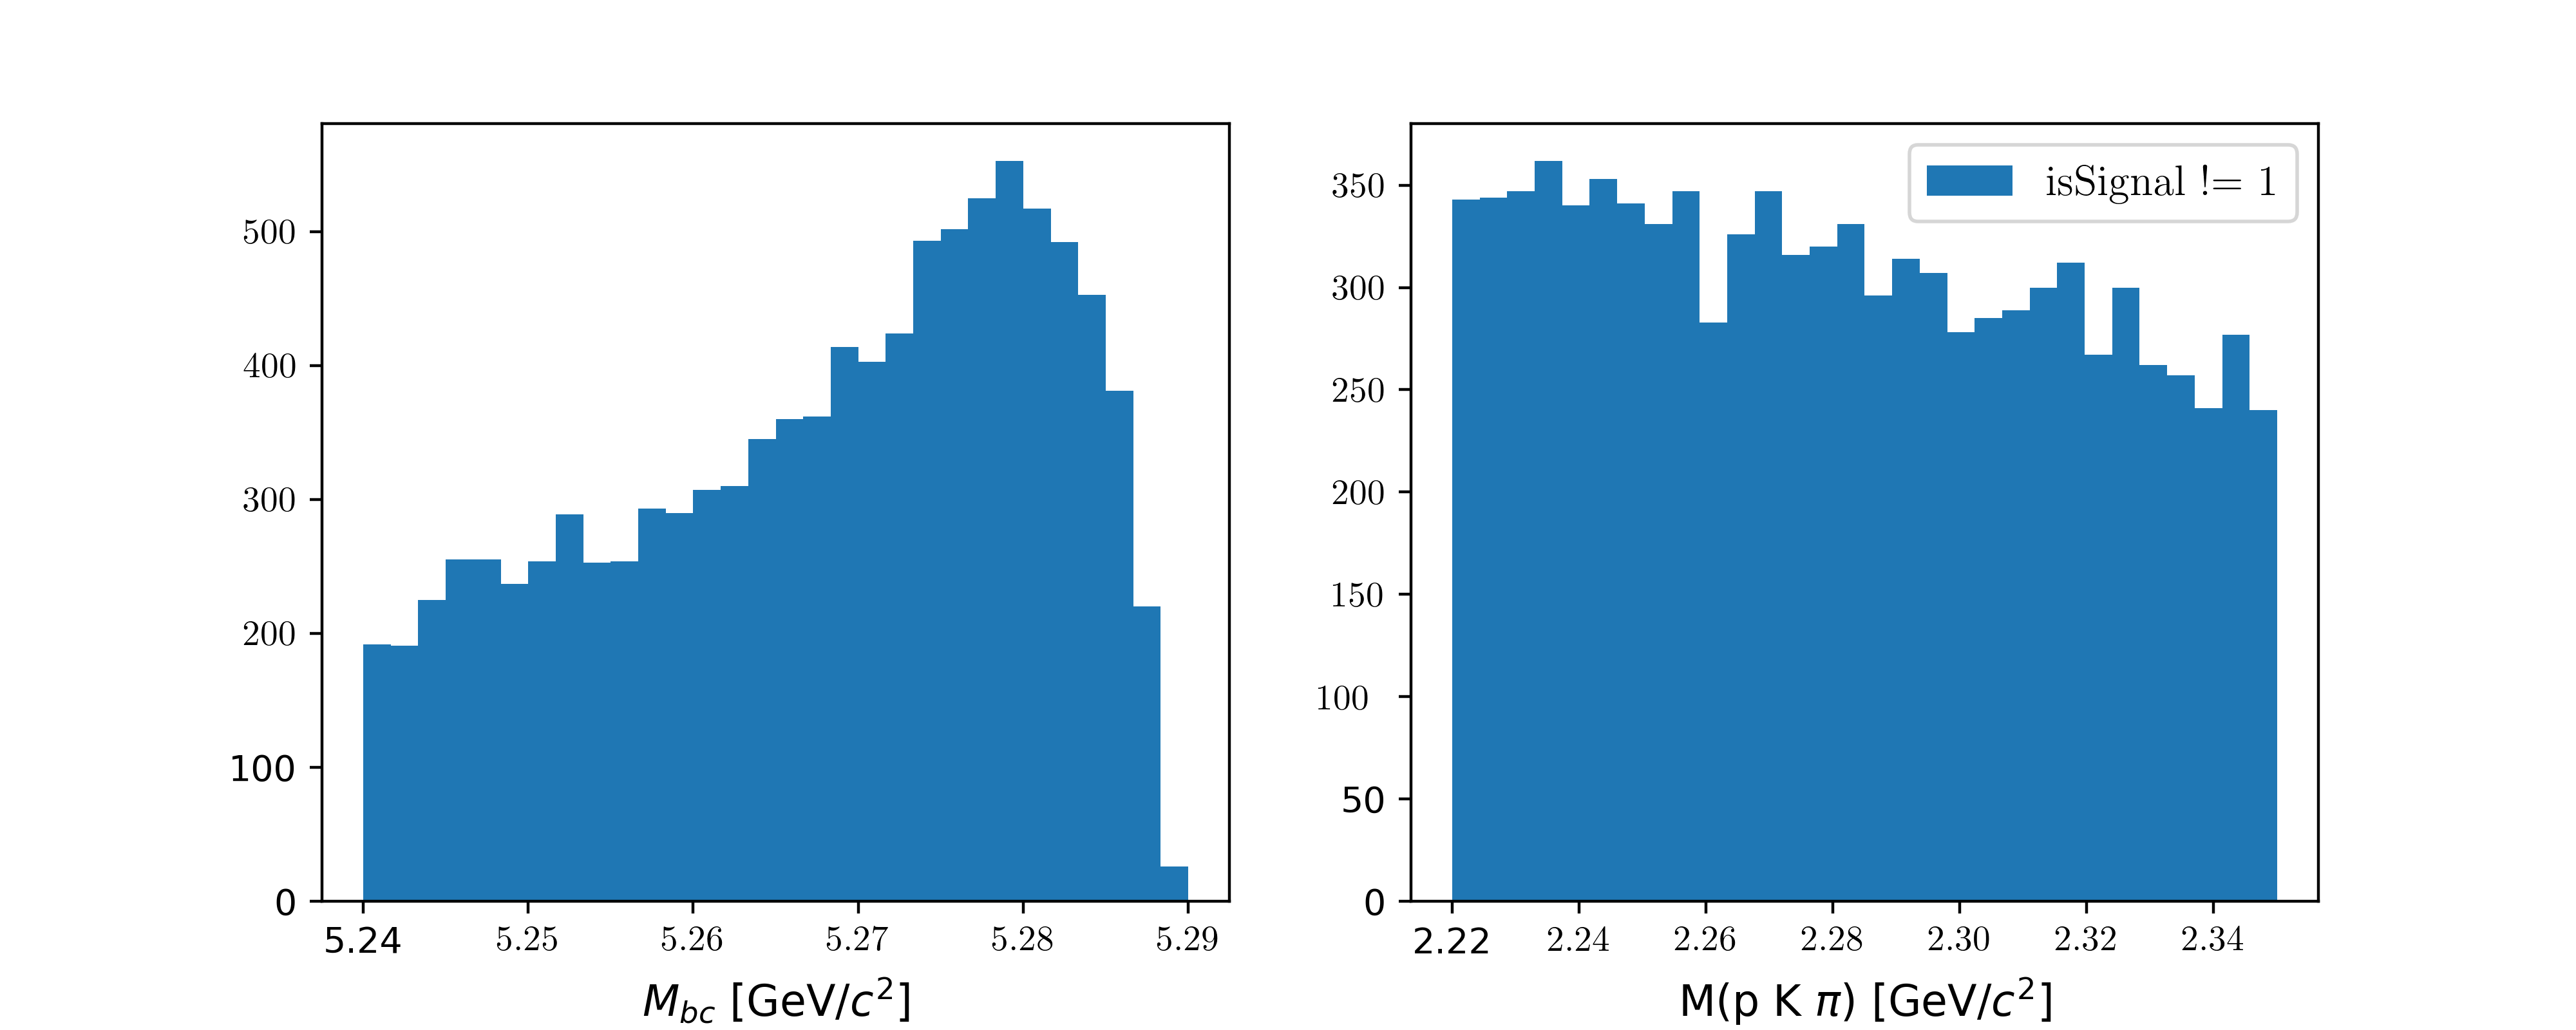
\includegraphics[width=1\textwidth]{04-chargedCorrBtoLambda/figs/chargedBcorr_CrossfeedNoLambdaCpeak.png}}
\caption{$M_{bc}$ and $M(p K \pi)$ of crossfeed events without $ \Lambda_c$ peak, i.e.: where $ \Lambda_c$ baryons were not present or not correctly reconstructed. }
\label{fig:chargedBcorr_CrossfeedNoLambdaCpeak}
\end{figure}

\noindent \cref{fig:5streams_Crossfeed_charged_corrLambdaC_2Dfit} shows the projections in $M_{bc}$  and $M(p K \pi)$ of the two dimensional fit of this type of background.
The $M_{bc}$ is modelled with a sum of Novosibirsk (colored in magenta) and Argus function (colored in red). Whereas the $M(p K \pi)$ distribution is described by the sum of a first order Chebychev polynomial and the peak by the same sum of three Gaussian functions used to describe the signal peak. In fact the latter is the result of the reconstruction of crossfeed events $B^0 \rightarrow \Lambda_c$.  Therefore the 2D PDF can be written as:\\

\begin{equation}
P^{CrossBkg}_{B,\Lambda_c}(M_{bc}, M(p K \pi)) = [\Gamma_{Nov}(M_{bc}) + \Gamma_{ARG}(M_{bc})] \times [\rho_{Cheb1}(M(p K \pi)) + \rho_{G}(M(p K \pi))]
\end{equation}

\begin{figure}[H]
\centering
{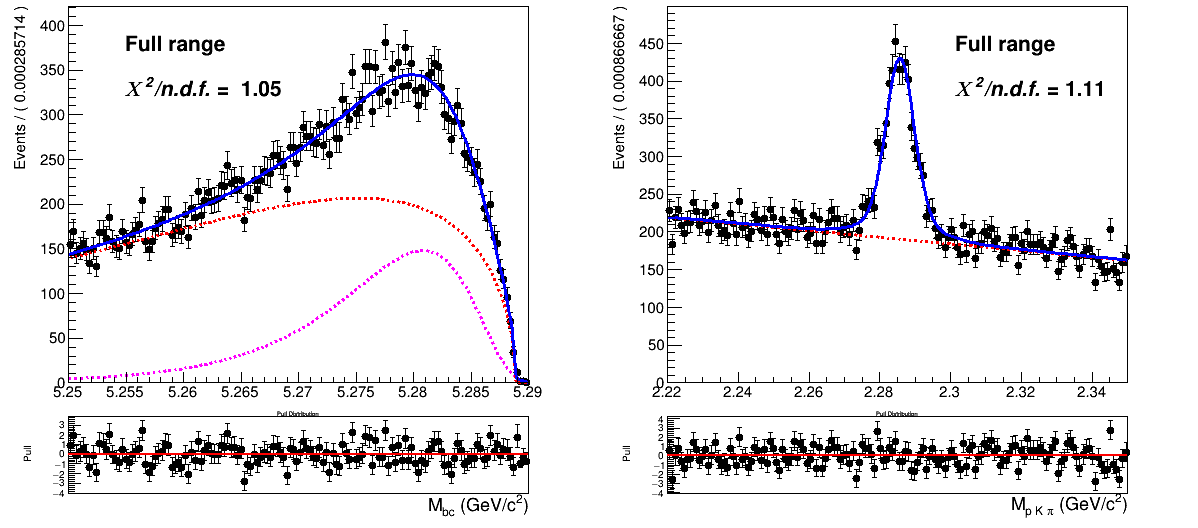
\includegraphics[width=0.8\textwidth]{04-chargedCorrBtoLambda/figs/stream12345_Crossfeed_charged_corrLambdaC_2Dfit.png}}
\caption{Two dimensional fit of crossfeed ($B^0\bar{B^0}$) events in $M_{bc}$  and $M(p K \pi)$. }
\label{fig:5streams_Crossfeed_charged_corrLambdaC_2Dfit}
\end{figure}


\begin{figure}[h!]
%\centering
{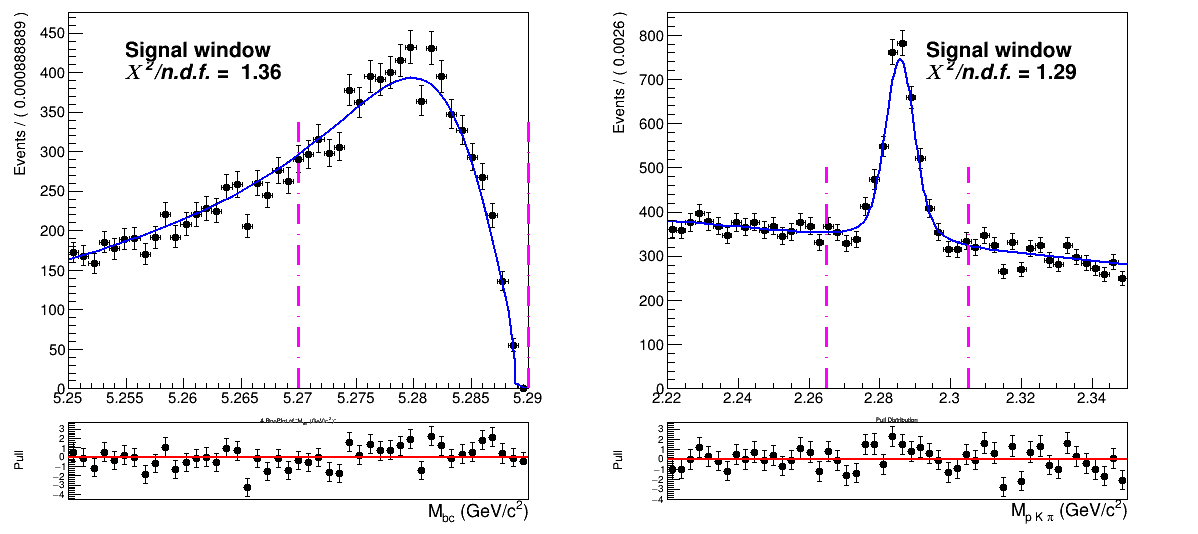
\includegraphics[width=0.8\textwidth]{04-chargedCorrBtoLambda/figs/Signal_window_stream12345_Crossfeed_charged_corrLambdaC_2Dfit.png}}
\caption{Signal region projections in $M_{bc}$ and $M(p K \pi)$. }
\label{fig:5streams_Signal_window_Crossfeed_charged_corrLambdaC_2Dfit}
\end{figure}

\begin{figure}[h!]
%\centering
{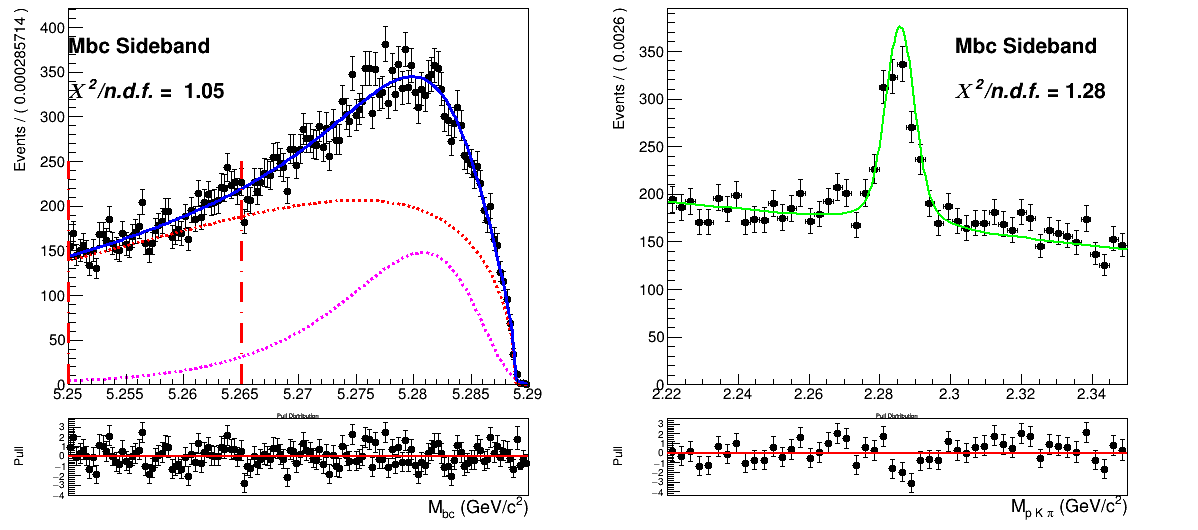
\includegraphics[width=0.8\textwidth]{04-chargedCorrBtoLambda/figs/Mbc_Sideband_stream12345_Crossfeed_charged_corrLambdaC_2Dfit.png}}
\caption{$M_{bc}$ sideband region projection. }
\label{fig:5streams_Mbc_Sideband_Crossfeed_charged_corrLambdaC_2Dfit}
\end{figure}

\noindent From the projections plotted in \cref{fig:5streams_Crossfeed_charged_corrLambdaC_2Dfit} the distributions appear to be well described by the PDF discussed above.
Though the agreement in the $\Lambda_c$ invariant mass is not fully respected when different regions of $M_{bc}$ are considered, as one can see from \cref{fig:5streams_Signal_window_Crossfeed_charged_corrLambdaC_2Dfit} and 
\cref{fig:5streams_Mbc_Sideband_Crossfeed_charged_corrLambdaC_2Dfit}. The fraction of the amount of peaking events is not uniform among different $M_{bc}$ regions. Since this background typology is peaking in both the observables of the fit, the potential correlation between them could have an impact on the signal yield extraction in the total fit. 

To minimize this effect, and to avoid possible biases deriving from this feature, a correction is attempted. The $M_{bc}$ is divided in 5 different regions. 
As shown in Figures \ref{fig:CrossfeedMbcRegionsInvMpeak1}-\ref{fig:CrossfeedMbcRegionsInvMpeak5}, for each of these regions a fit on the projected $\Lambda_c$ invariant mass 
is performed to extract 5 values of the fraction of peaking events in those regions (all other parameters are fixed). Those values are then used for a parametrization of this 
parameter as a function of $M_{bc}$. \\
\noindent From the plot shown in \cref{fig:InvMpeak_fraction_linearFit} one can see that it is possible to describe the trend with a linear dependence with a good approximation.

\begin{figure}[H]
\centering
{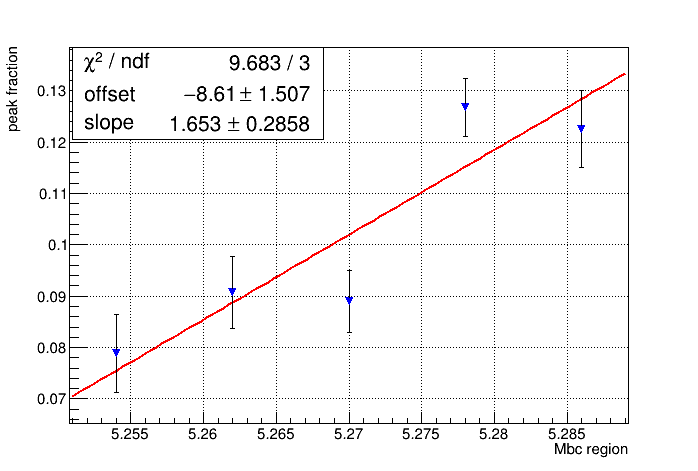
\includegraphics[width=0.6\textwidth]{04-chargedCorrBtoLambda/figs/streams12345_chargedCorrLambdaC_Crossfeed_InvM_frac_param.png}}
\caption{Invariant mass peak fraction as a function of $M_{bc}$. }
\label{fig:InvMpeak_fraction_linearFit}
\end{figure}

\begin{figure}[H]
\centering
\subcaptionbox{\label{fig:CrossfeedMbcRegionsInvMpeak1}}
{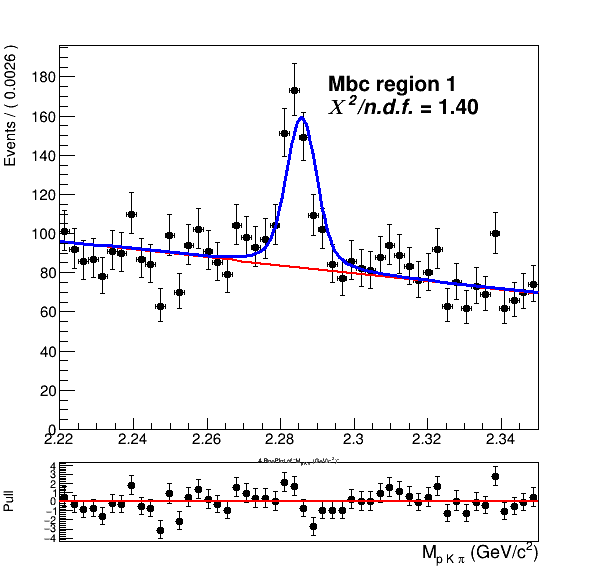
\includegraphics[width=.4\textwidth]{04-chargedCorrBtoLambda/figs/region1_stream12345_Crossfeed_charged_corrLambdaC_2Dfit.png}} 
\subcaptionbox{\label{fig:CrossfeedMbcRegionsInvMpeak2}}
{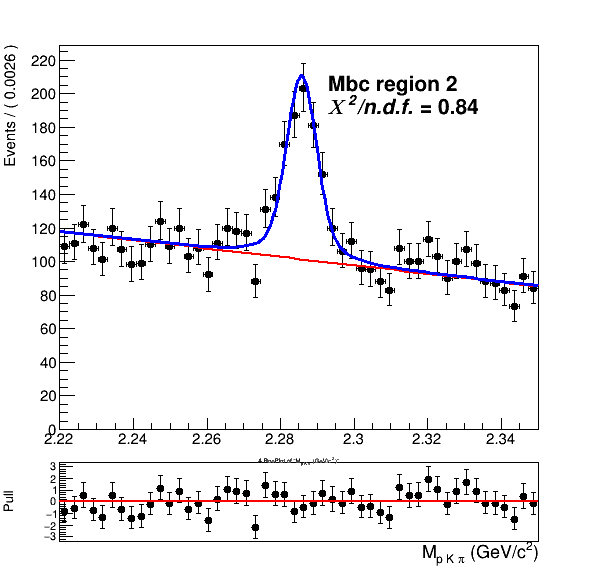
\includegraphics[width=.4\textwidth]{04-chargedCorrBtoLambda/figs/region2_stream12345_Crossfeed_charged_corrLambdaC_2Dfit.png}}
\subcaptionbox{\label{fig:CrossfeedMbcRegionsInvMpeak3}}
{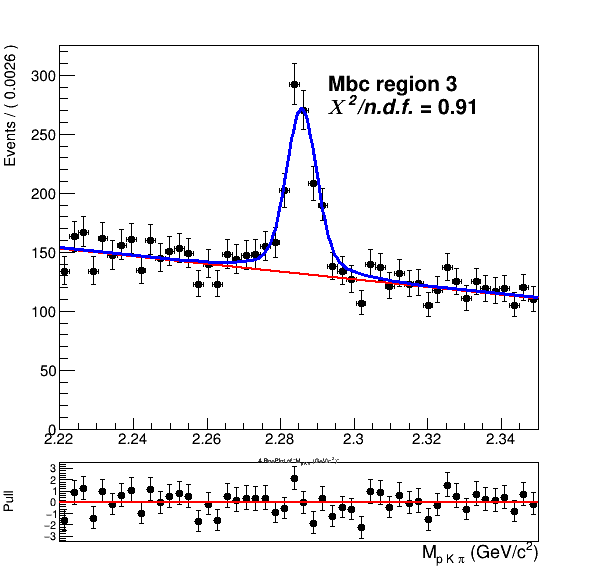
\includegraphics[width=.4\textwidth]{04-chargedCorrBtoLambda/figs/region3_stream12345_Crossfeed_charged_corrLambdaC_2Dfit.png}}
\subcaptionbox{\label{fig:CrossfeedMbcRegionsInvMpeak4}}
{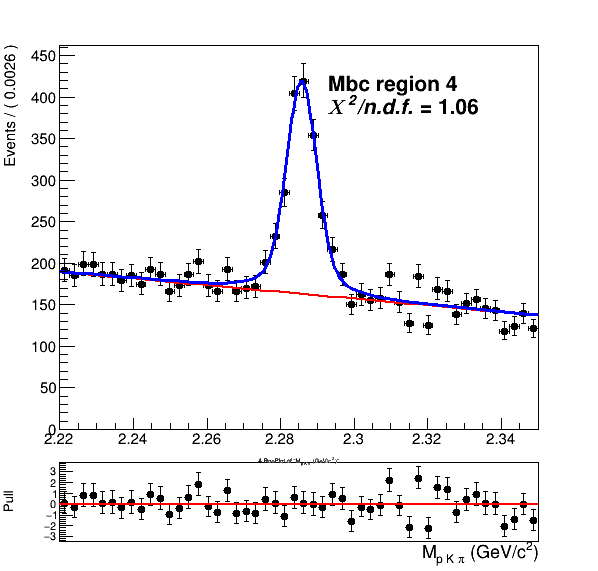
\includegraphics[width=.4\textwidth]{04-chargedCorrBtoLambda/figs/region4_stream12345_Crossfeed_charged_corrLambdaC_2Dfit.png}}
\subcaptionbox{\label{fig:CrossfeedMbcRegionsInvMpeak5}}
{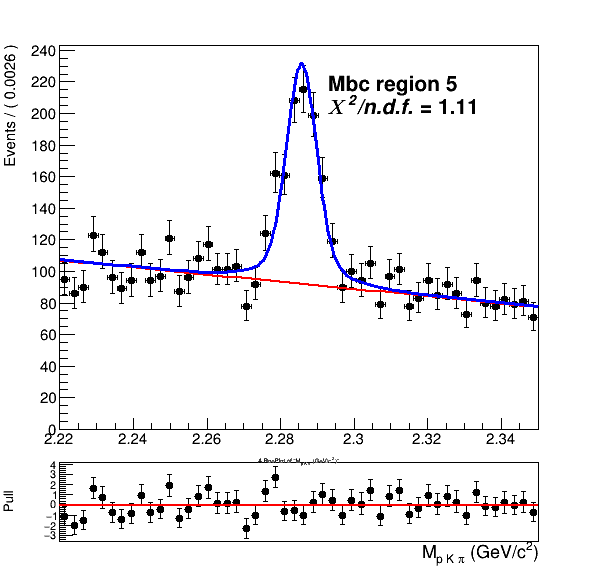
\includegraphics[width=.4\textwidth]{04-chargedCorrBtoLambda/figs/region5_stream12345_Crossfeed_charged_corrLambdaC_2Dfit.png}}
\caption{Fits of $M(p K \pi)$ in 5 different regions of $M_{bc}$: $5.25 < M_{bc} < 5.258$ GeV/c$^2$, $5.258 < M_{bc} < 5.266$ GeV/c$^2$, $5.266 < M_{bc} < 5.274$ GeV/c$^2$, $5.274 < M_{bc} < 5.282$ GeV/c$^2$,  $5.282 < M_{bc} < 5.29$ GeV/c$^2$.}
\end{figure}

The 2D PDF describing the crossfeed background is consequently modified:\\
\begin{equation}\label{eq:paramCrossfeedPDF}
P^{CrossBkg}_{B,\Lambda_c}(M_{bc}, M(p K \pi)) = [\Gamma_{Nov}(M_{bc}) + \Gamma_{ARG}(M_{bc})] \times [F(M(p K \pi)|M_{bc})]
\end{equation}
where the conditional PDF $F(M(p K \pi)|M_{bc})$ describing the invariant mass is still a sum of $\rho_{Cheb1}(M(p K \pi))$ and $ \rho_{G}(M(p K \pi))$, but their fraction is now parametrized as a function of  $M_{bc}$.\\
In Figures \ref{fig:correctedSignal_window_Crossfeed_charged_corrLambdaC}- \ref{fig:corrrectedMbc_Sideband_stream12345_Crossfeed_charged_corrLambdaC} one can appreciate the improvement obtained with this correction.  

\begin{figure}[h!]
%
{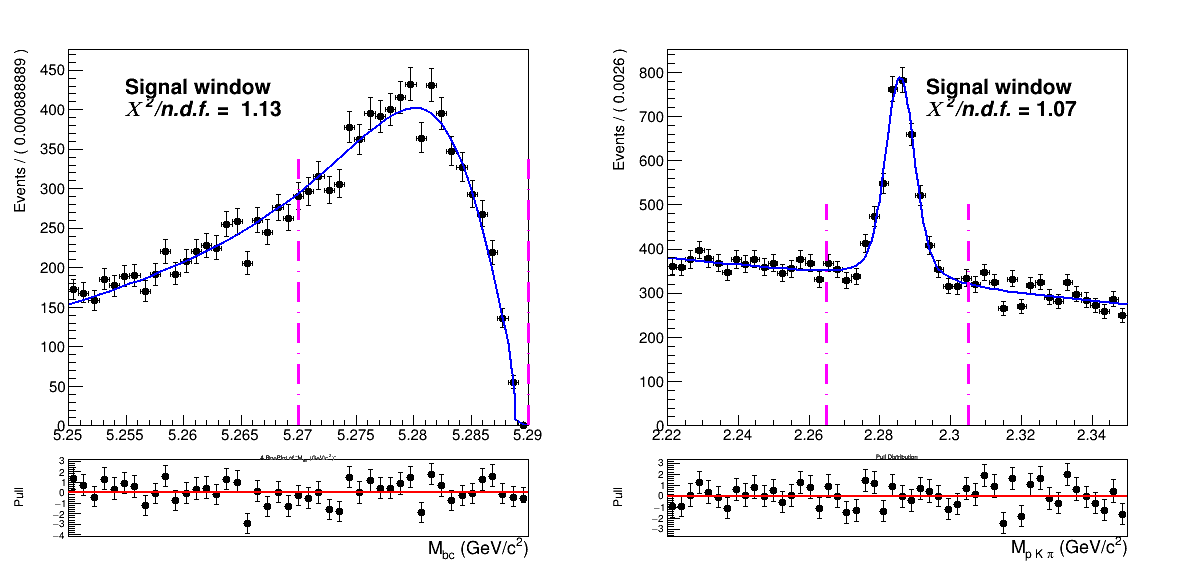
\includegraphics[width=0.75\textwidth]{04-chargedCorrBtoLambda/figs/Signal_window_stream12345_Crossfeed_charged_corrLambdaC_2Dfit_afterParametrization.png}}
\caption{Signal region projections in $M_{bc}$ and $M(p K \pi)$ after the parametrization. }
\label{fig:correctedSignal_window_Crossfeed_charged_corrLambdaC}
\end{figure}

\begin{figure}[H]
%\centering
{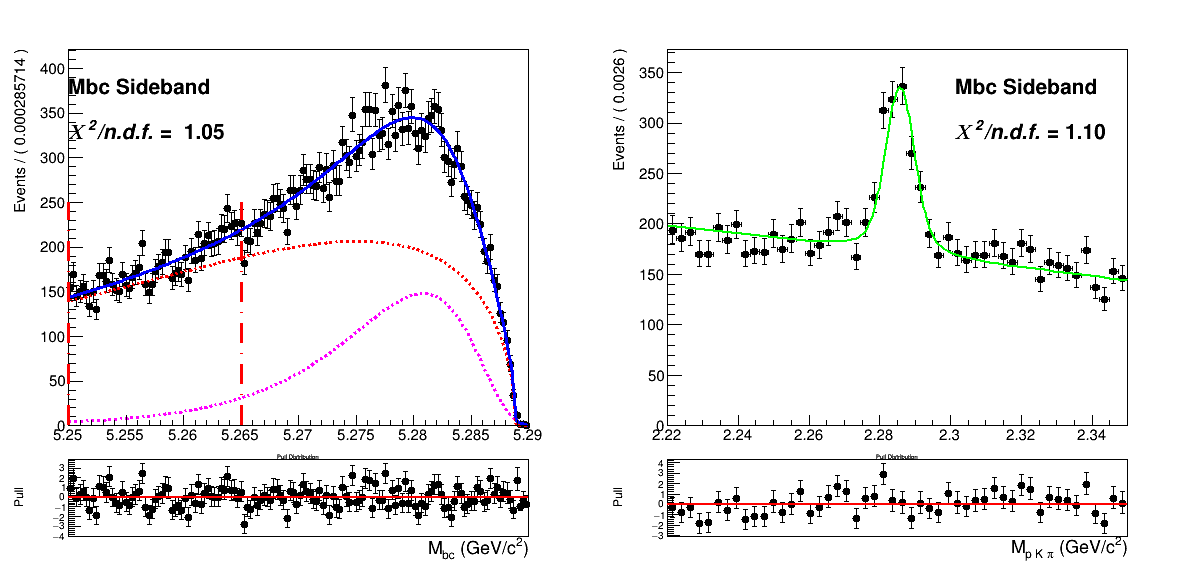
\includegraphics[width=0.8\textwidth]{04-chargedCorrBtoLambda/figs/Mbc_Sideband_stream12345_Crossfeed_charged_corrLambdaC_2Dfit_afterParametrization.png}}
\caption{$M_{bc}$ sideband region projection after the parametrization. }
\label{fig:corrrectedMbc_Sideband_stream12345_Crossfeed_charged_corrLambdaC}
\end{figure}


%\newpage

\noindent \textbf{Continuum background}
\newline
Besides the dataset recorded at the energy of the $\Upsilon(4S) $ resonance  ($E^{on-res}
_{CMS} = $ 10.58 GeV), the \textit{Belle} experiment recorded a sample of 89.4 $fb^{-1}$ at an energy 60 MeV below the nominal  $\Upsilon(4S) $ resonance ($E^{off-res}_{CMS} = $ 10.52 GeV). The dataset allows to check for an appropriate modeling of the continuum MC simulation. %, by comparing the off-resonance data with the MC expectation for the continuum background. 
Using the official tables \newline ( \url{https://belle.kek.jp/secured/nbb/nbb.html}) the off-resonance sample is scaled by 

\begin{equation}
    \frac{\mathcal{L}^{on-res}}{\mathcal{L}^{off-res}} \left( \frac{E^{off-res}_{CMS}}{E^{on-res}_{CMS}}\right)^2
\label{eq:off-resScaling}
\end{equation}


\noindent taking into account the difference in luminosity and in $E_{CMS}$ (Energy in center of mass system).


\begin{figure}[h!]
%\centering
{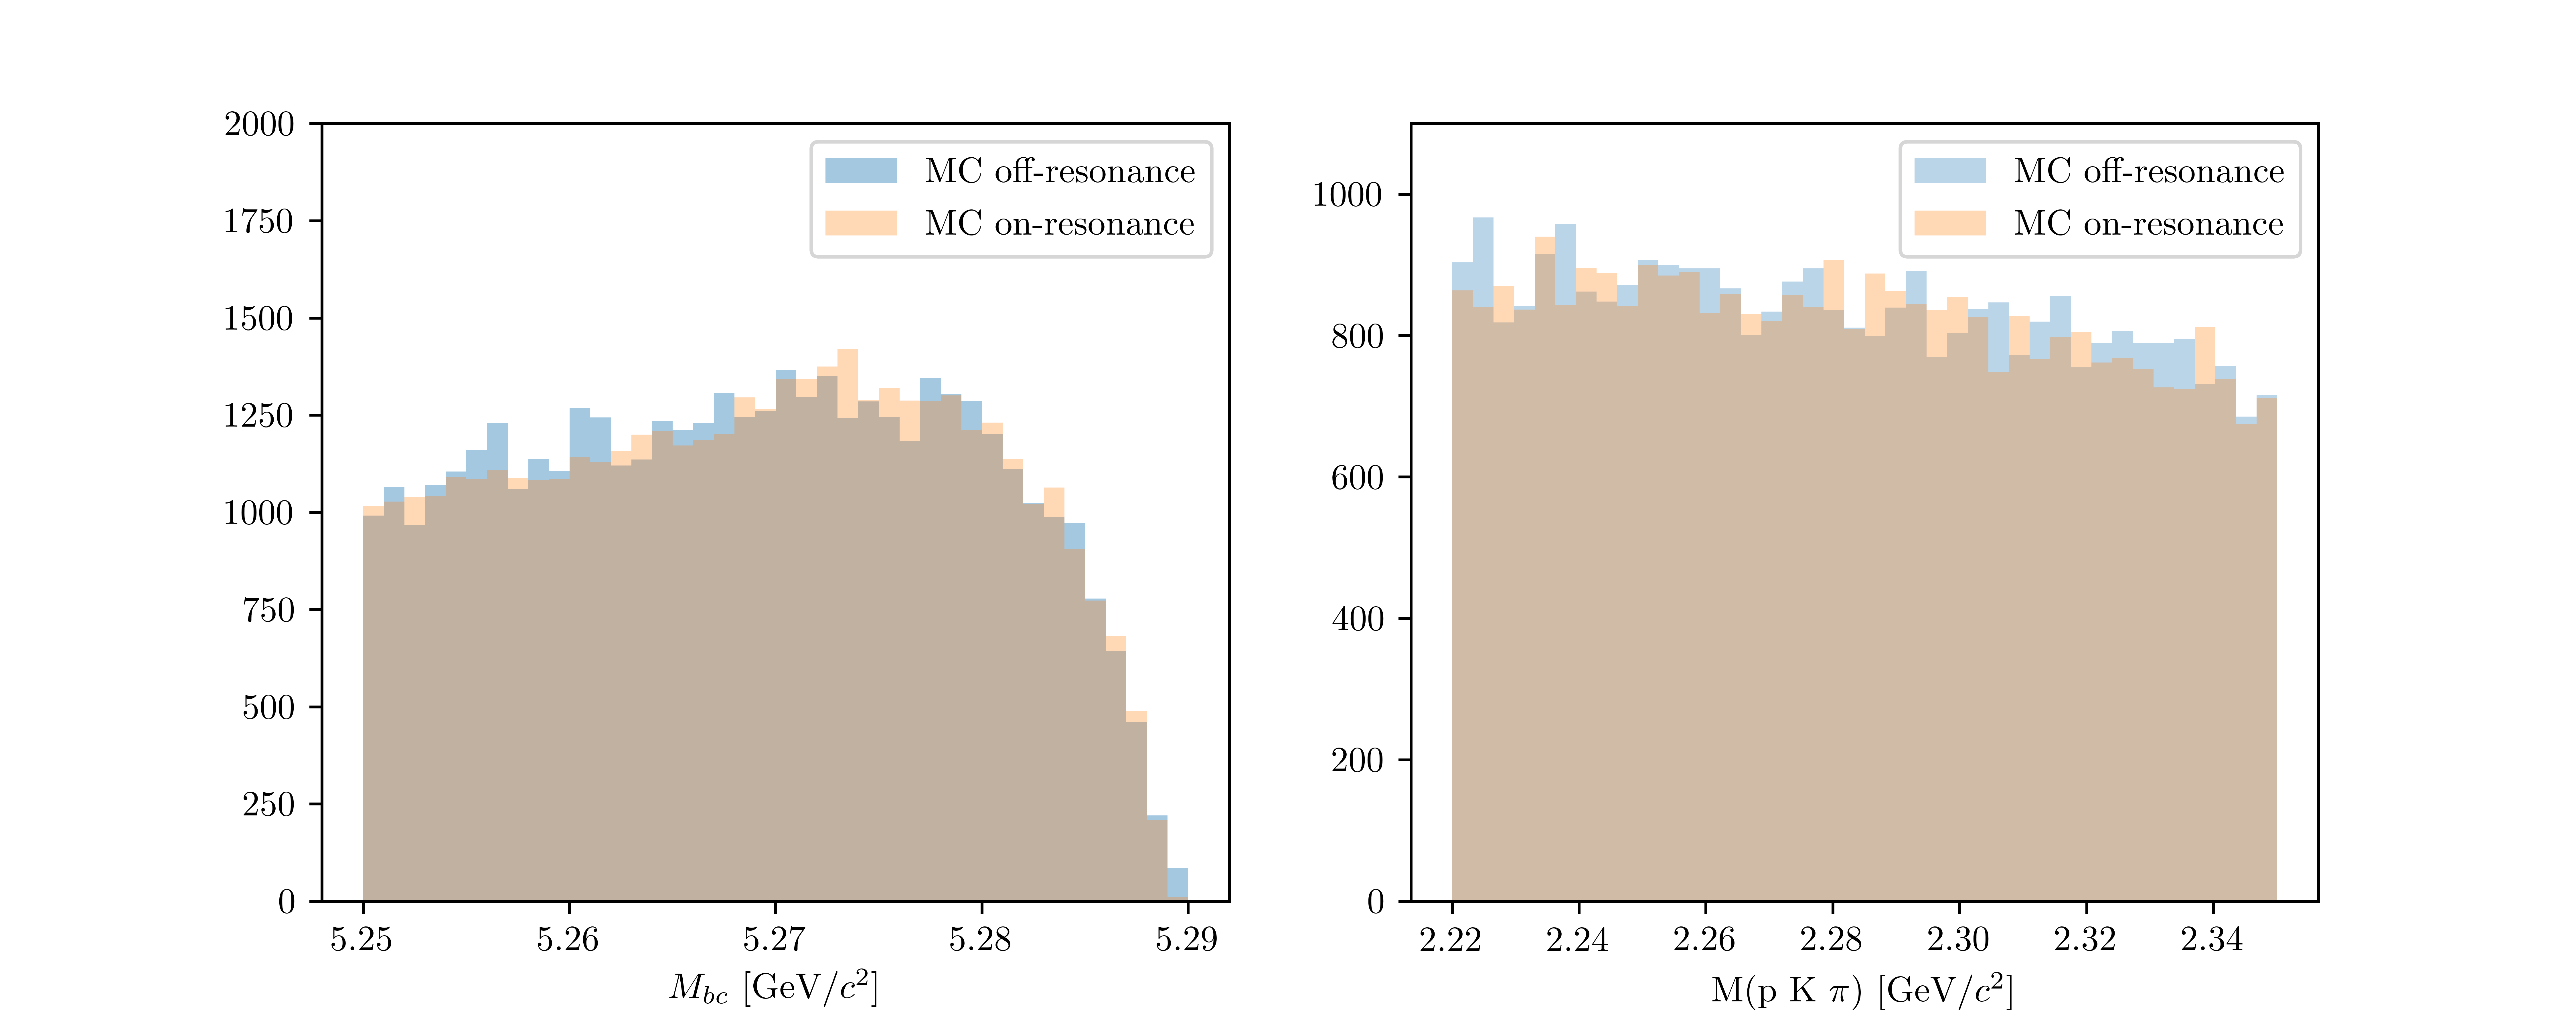
\includegraphics[width=1.05\textwidth]{04-chargedCorrBtoLambda/figs/MbcInvM_MC_on_off-resonance_comparison.png}}
\caption{$M_{bc}$ and $M(p K \pi)$ comparison between  on-/off-resonance (scaled) Monte Carlo simulated continuum. The scaling is applied according to \cref{eq:off-resScaling} and shifting the $M_{bc}$ distribution by $E^{on-res}_{CMS} - E^{off-res}_{CMS}$. }
\label{fig:MbcInvM_MC_on_off-resonance_comparison}
\end{figure} 

\noindent The plot in Fig.\ref{fig:MbcInvM_MC_on_off-resonance_comparison} shows the $M_{bc}$ and $M(p K \pi)$ distributions in the MC on-/off-resonance continuum after the scaling\footnote{it is obtained with the MC off-resonance sample being composed of 6 streams: the total amount is normalized}.

Ideally, provided that there's a good agreement between MC and data for the off-resonance sample and also between the MC  on-/off-resonance continuum after the scaling, one could directly use the scaled off-resonance data to describe the continuum background in the fit on data. There are two reasons that prevent this very straightforward approach:
\begin{itemize}

\item First, since the off-resonance MC (and data) present very low statistics (Fig. \ref{fig:off-resData_charged_corrLambdaC_InvM} shows the  $\Lambda_c$ 
invariant mass in off-resonance data), scaling them with all the applied selection cuts would cause the PDF describing the continuum to be very much affected by statistical fluctuations. 
\item Secondly, the $B$ meson candidates are reconstructed in both on-resonance and off-resonance events for values of $M_{bc} \geq 5.22 $ GeV/c$^2$, but the $E_{CMS}$ differs: there can be effects of correlations between the applied \textit{SignalProbability} cut and the $M_{bc}$ variable that one needs to take into account. %This effects on the $M_{bc}$ are carefully studied in the analysis of the control sample. 
\end{itemize}

\begin{figure}[H]
%\centering
{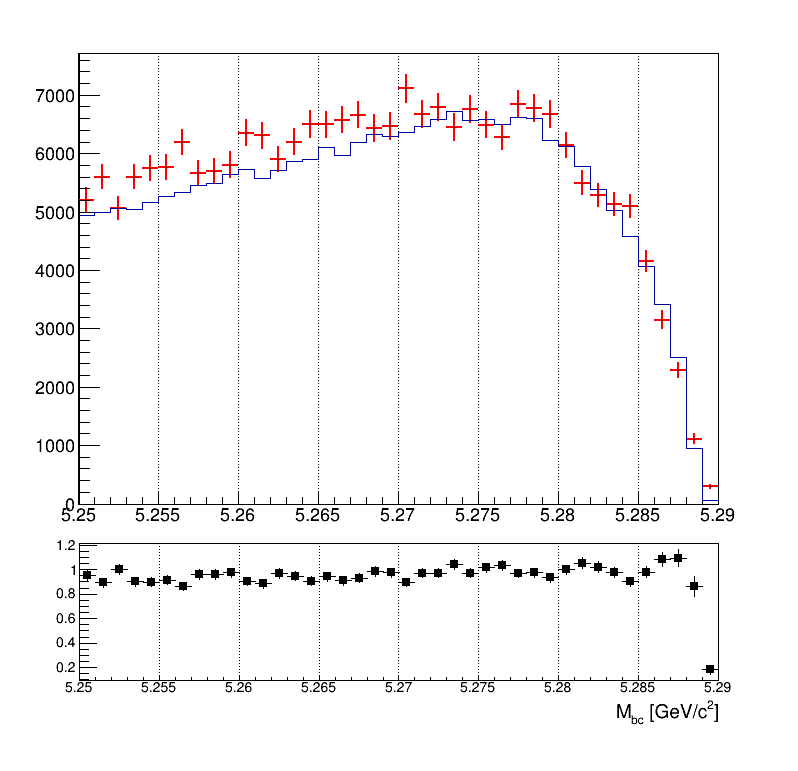
\includegraphics[width=0.5\textwidth]{04-chargedCorrBtoLambda/figs/stream01234_Mbc_continuumRescaling.png}}
\caption{$M_{bc}$ distributions of the MC (scaled) off-resonance sample (in red) and on-resonance (in blue) using 5 streams statistics and all nominal selection cuts applied.}
\label{fig:charged_corrLambdaC_Mbc_on_offResScaled}
\end{figure}



\begin{figure}
\centering
\subcaptionbox{\label{fig:off-resData_charged_corrLambdaC_InvM}}
{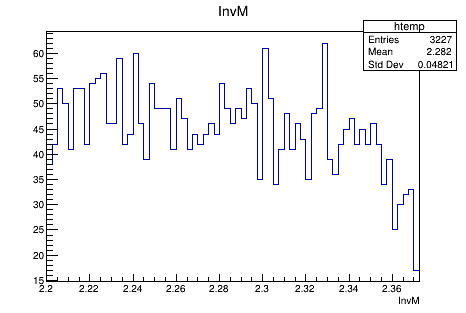
\includegraphics[width=.46\textwidth]{04-chargedCorrBtoLambda/figs/chargedCorrLambdaC_off-resData.png}}\quad
\subcaptionbox{\label{fig:off-resData_charged_corrLambdaC_InvM_woCS}}
{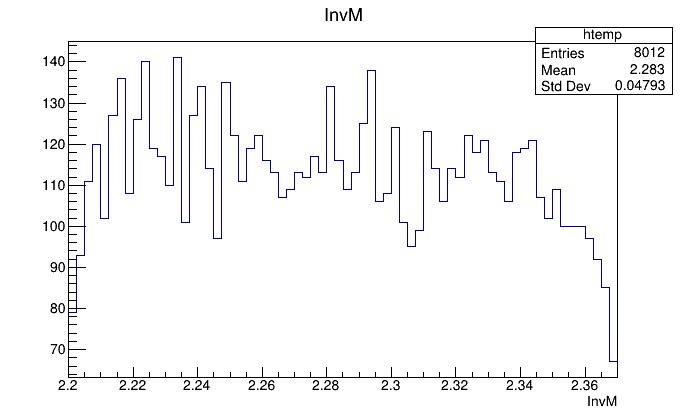
\includegraphics[width=.48\textwidth]{04-chargedCorrBtoLambda/figs/chargedCorrLambdaC_off-resData_woCScuts.png}} \quad
\caption{On the left: $\Lambda_c$ invariant mass in off-resonance data (all nominal cuts applied). On the right: $\Lambda_c$ invariant mass in off-resonance data after the continuum suppression cut removal.}
\end{figure}


In Fig. \ref{fig:charged_corrLambdaC_Mbc_on_offResScaled} one can notice some discrepancy in the shapes, apart from the not negligible statistical fluctuations in the (scaled) off-resonance distribution.  
In the $\Lambda_c$ invariant mass one doesn't expect correlation effects, but nevertheless there can be differences due to the limited statistics of the off-resonance sample. In fact, in the case of on-resonance MC some events in which  $\Lambda_c$ candidates survive nominal selection cuts are visible and can be described with a small Gaussian on the top of the flat background (Fig.\ref{fig:onRes_InvM_corrLambdaC}). On the contrary the off-resonance sample doesn't show anything else beside the flat background (the Fig.\ref{fig:5streams_offRes_InvM_corrLambdaC} shows a 5 streams statistics).


\newpage


\begin{figure}
\centering
\subcaptionbox{\label{fig:onRes_offResScaledMbc_corrLambdaC}}
{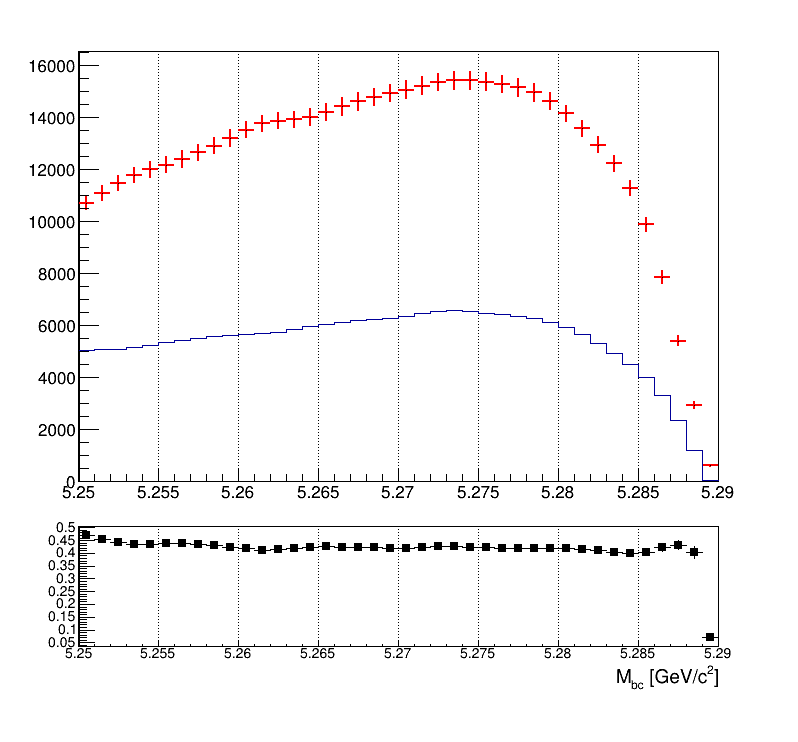
\includegraphics[width=.46\textwidth]{04-chargedCorrBtoLambda/figs/stream01235_charged_corrLambdaC_woCScuts_Mbc_scaling.png}} \quad
\subcaptionbox{\label{fig:Mbc_scaled_bin_correctedOffResContinuum}}
{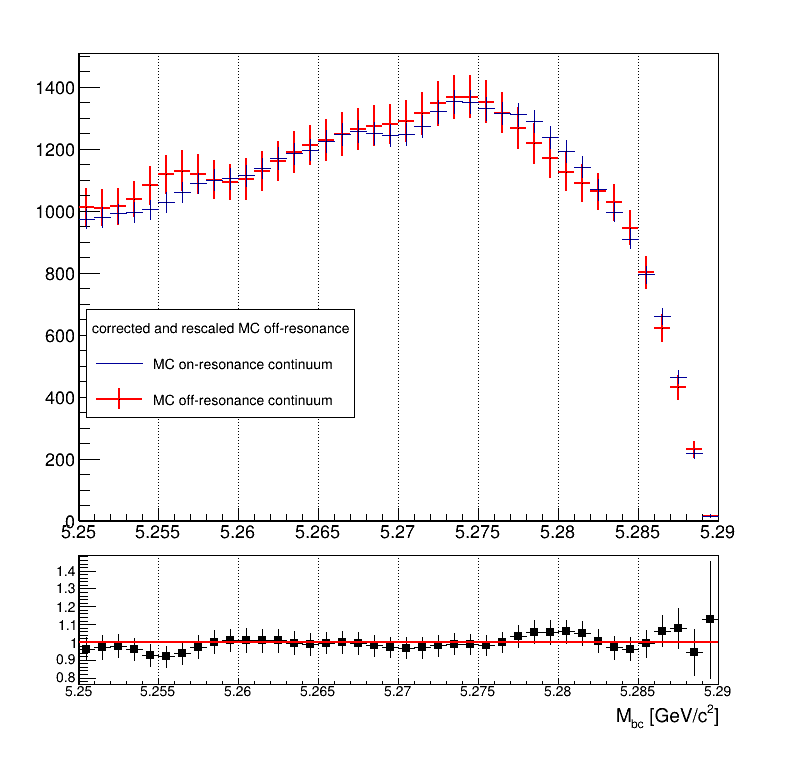
\includegraphics[width=.44\textwidth]{04-chargedCorrBtoLambda/figs/MC_on_off_resonance_stream4_continuum_2D_Mbc_corrected.png}} \quad
\caption{On the left: $M_{bc}$ distributions of the MC off-resonance sample without continuum suppression and the MC continuum sample with applied continuum suppression. On the right: $M_{bc}$ distributions of the corrected scaled MC off-resonance and on-resonance MC continuum.}
\end{figure}


The procedure adopted to obtain the PDF describing the continuum background  $M_{bc}$ distribution is the following:
\begin{itemize}

\item 5 streams of off-resonance MC were scaled according to \cref{eq:off-resScaling} without continuum suppression being applied and compared to the distribution of 5 streams of on-resonance continuum
\item From a ratio plot, like the one in Fig. \ref{fig:onRes_offResScaledMbc_corrLambdaC}, the bin-correction is obtained to correct the off-resonance data in the scaling procedure.
To obtain the shape that can describe the continuum background  $M_{bc}$ distribution on data the continuum suppression is not applied on the off-resonance continuum sample, in order to acquire more statistics. 
\end{itemize}

\noindent This procedure is first tested on an independent MC sample (see Fig. \ref{fig:Mbc_scaled_bin_correctedOffResContinuum} ) to check the result on simulated data before applying it on data.





The validity of the method relies on the fact that  on-/off-resonance continuum events are well modeled in MC and that the shape of the $M_{bc}$ distribution doesn't change significantly when removing the continuum suppression cut both on MC and data (as one can see from Figures \ref{fig:corrLambdaC_OffResonance_w_wo_CS_comparison_5streams} - \ref{fig:corrLambdaC_OffResonance_w_wo_CS_comparison_Data}).
Additionally, the continuum suppression cut efficiency should be the same in data and MC in order to have the correct scaling on data with the above mentioned method. Fig. \ref{fig:R2_MC-Data_off_resonance_distributions} shows the distribution of the $foxWolframR2$ variable in off-resonance MC and data. The slight shift visible in data can cause a different impact on data in terms of rejected continuum background when applying the $foxWolframR2 < 0.3$ cut. It is found to reject about 60$\%$ of the continuum background in data, whereas it rejects 55$\%$ of the continuum background in MC ( 56$\%$ in on-resonance MC). Therefore in data one can expect about 2.25$\%$ less continuum background events. This discrepancy is not statistical significant (the statistical uncertainty for the continuum background events is of the level of $\sim 1\%$),  a simple correction to the number of events can be applied on data and its possible systematics can be then taken into account.% can be then taken into account when fitting the data sample, applying a simple correction to the number of events. %However, being the number of events in the off-resonance data sample without the continuum suppression applied very small (less than $10^4$), the uncertainty in the mentioned fraction of events is negligible compared to the statistical uncertainty on the on-resonance continuum background events in MC


\begin{figure}
\centering
\subcaptionbox{\label{fig:corrLambdaC_OffResonance_w_wo_CS_comparison_5streams}}
{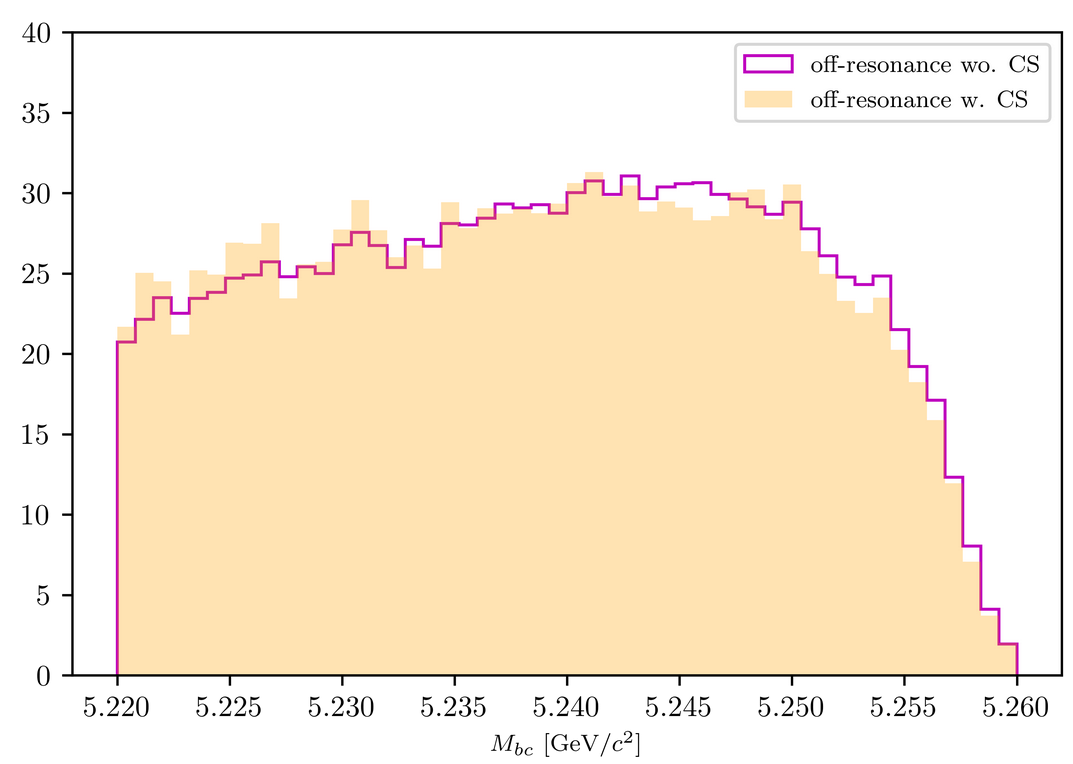
\includegraphics[width=.65\textwidth]{04-chargedCorrBtoLambda/figs/corrLambdaC_OffResonance_w_wo_CS_comparison_5streams.png}} 
\subcaptionbox{\label{fig:corrLambdaC_OffResonance_w_wo_CS_comparison_Data}}
{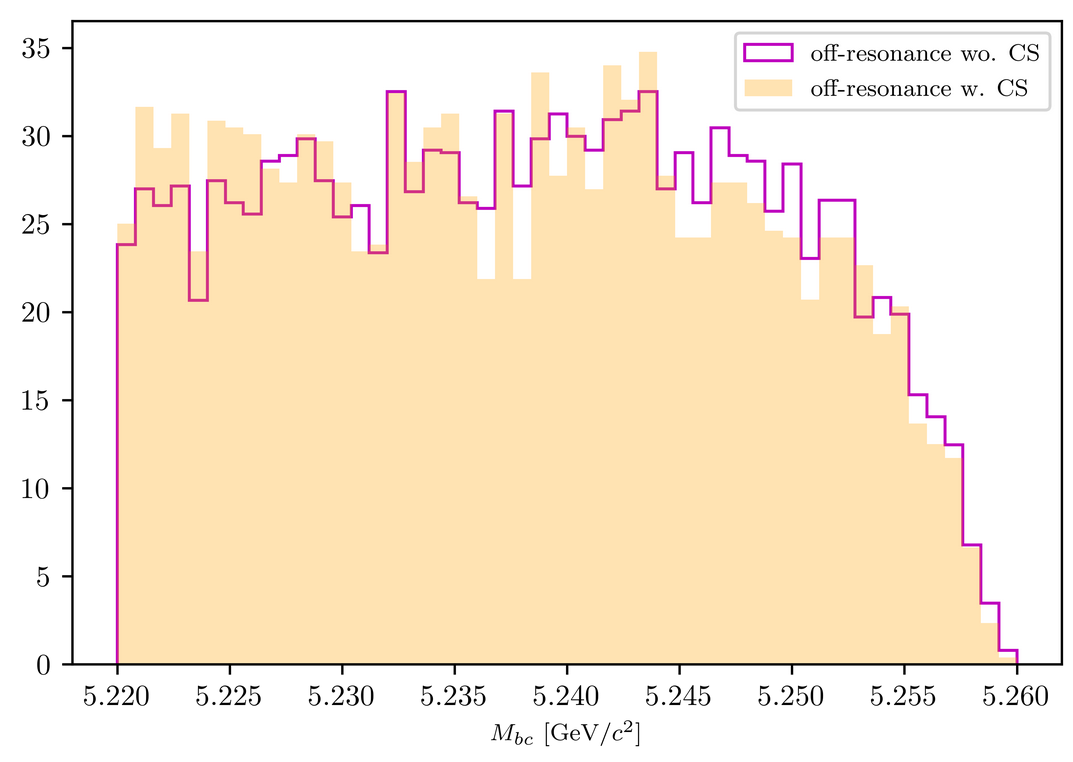
\includegraphics[width=.65\textwidth]{04-chargedCorrBtoLambda/figs/corrLambdaC_OffResonance_w_wo_CS_comparison_Data.png}} 
\caption{Above: $M_{bc}$ distributions of the MC off-resonance sample (5 streams) with and without continuum suppression. Below: $M_{bc}$ distributions on data with and without continuum suppression.}
\end{figure}



\begin{figure}[h!]
%\centering
{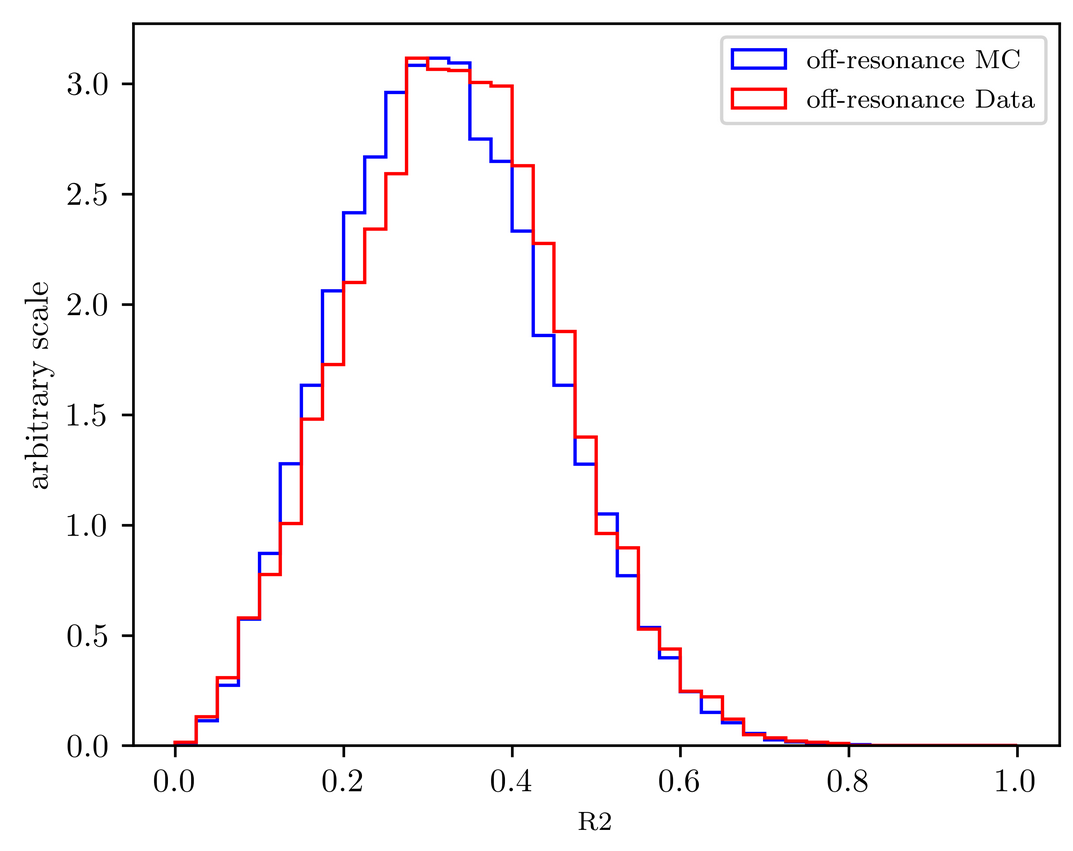
\includegraphics[width=0.5\textwidth]{04-chargedCorrBtoLambda/figs/R2_MC-Data_off_resonance_distributions.png}}
\caption{Distributions of variable $foxWolframR2$ in off-resonance MC and data.}
\label{fig:R2_MC-Data_off_resonance_distributions}
\end{figure}




%One can see that with this method the scaled simulated off-resonance events agree at reasonable level with the simulated on-resonance continuum. 
 \noindent  The obtained distribution can be then fitted (see Fig. \ref{fig:charged_corrLambdaC_Mbc_continuumMC_fit}), i.e. with a Novosibirsk function. \\
This is the procedure which can be then applied on the off-resonance data to obtain the $M_{bc}$ shape describing the continuum background in data.
\begin{figure}[h!]
%\centering
{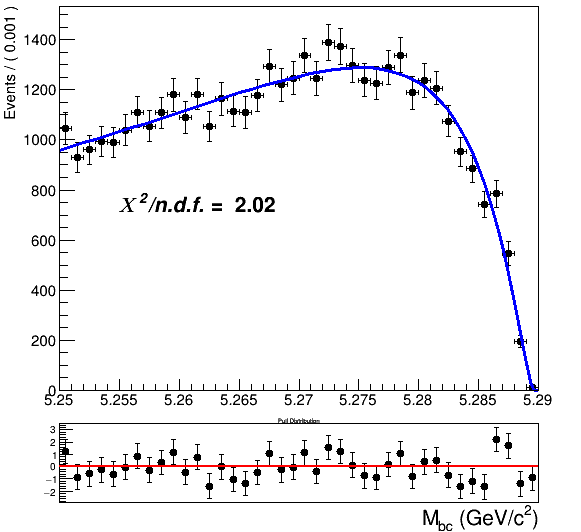
\includegraphics[width=0.45\textwidth]{04-chargedCorrBtoLambda/figs/stream5_rescaledMbc_40binsHist.png}}
\caption{Fit of the $M_{bc}$ distribution   MC (scaled) off-resonance continuum (one stream).}
\label{fig:charged_corrLambdaC_Mbc_continuumMC_fit}
\end{figure}


\newpage
The shape describing the $\Lambda_c$ invariant mass is obtained from the simulated on-resonance continuum, again using 5 streams statistics (see Fig. \ref{fig:onRes_InvM_corrLambdaC} ).
% Actually the cut discarding most of the true Λc(D⁰) in the continuum bkg is the one on signal probability. This is due to the fact that not being any true B mesons in ccbar events, most of the fake reconstructed ones have low signal probability (the cut on momenta cuts most of the fake D0s)

\begin{figure}
\centering
\subcaptionbox{\label{fig:onRes_InvM_corrLambdaC}}
{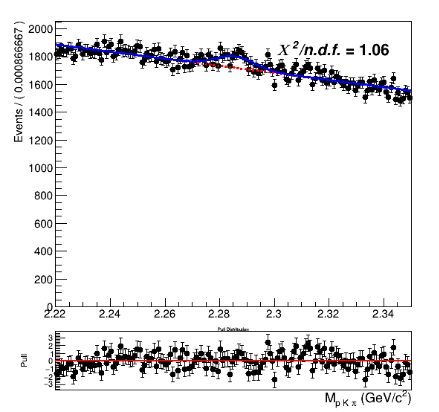
\includegraphics[width=.45\textwidth]{04-chargedCorrBtoLambda/figs/onRes_InvM_corrLambdaC.png}} 
\subcaptionbox{\label{fig:5streams_offRes_InvM_corrLambdaC}}
{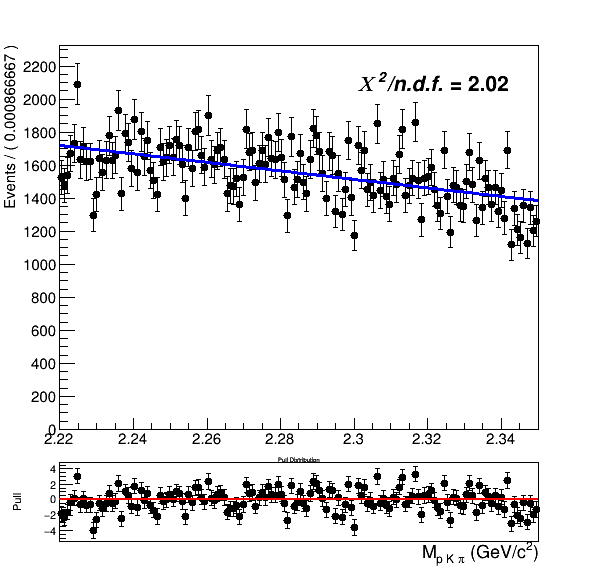
\includegraphics[width=.46\textwidth]{04-chargedCorrBtoLambda/figs/5streams_Off_resonanceRescaledContinuum_charged_corrLambdaC_oneGaussianInvMfit.png}} 
\caption{Comparison between 5 streams of MC on-resonance continuum \ref{fig:onRes_InvM_corrLambdaC}) and off-resonance (scaled) continuum in $M(p K \pi)$ (\ref{fig:5streams_offRes_InvM_corrLambdaC}).}
%\label{}
\end{figure}



Finally, it is possible to examine the validity of the whole procedure on the independent stream. 
Fig. \ref{fig:stream3corrLambddaC_total_continuum_2DFit} shows the $M_{bc}$, $M(p K \pi)$ projections of the two dimensional fit with the one-dimesional PDFs obtained with the above described procedure.
The 2D PDF used can be written as: \\
 \vspace{0.2 cm}

$P^{Continuum}_{B,\Lambda_c}(M_{bc}, M(p K \pi)) = \Gamma_{Nov}(M_{bc}) \times [\rho_{Cheb1}(M(p K \pi) + \rho_{G1}(M(p K \pi))]$\\
\vspace{0.2 cm}

where, as already anticipated, the invariant mass is described by a sum of a first order Chebychev polynomial and the peak by a single Gaussian function.

\begin{figure}[H]
  \begin{subfigure}{7cm}
    \centering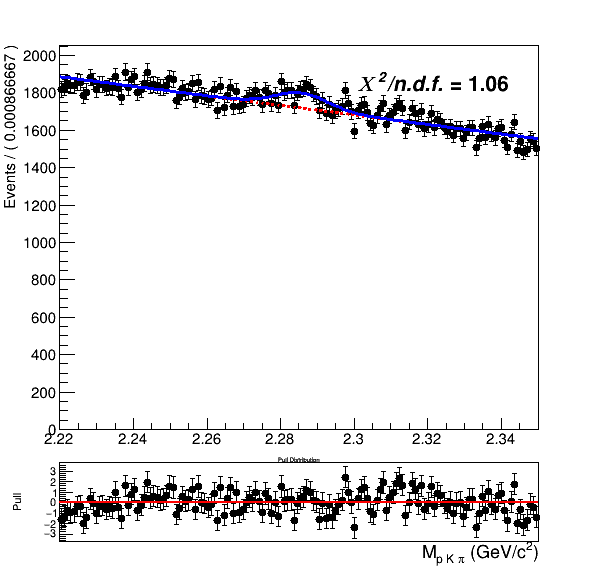
\includegraphics[width=6.5cm]{04-chargedCorrBtoLambda/figs/stream01234Continuum_charged_corrLambdaC_oneGaussianInvMfit.png}
   
    \label{fig:charged_corrLambdaC_InvM_continuumMC_1Gaussianfit}
  \end{subfigure}
  \begin{subfigure}{7cm}
    \centering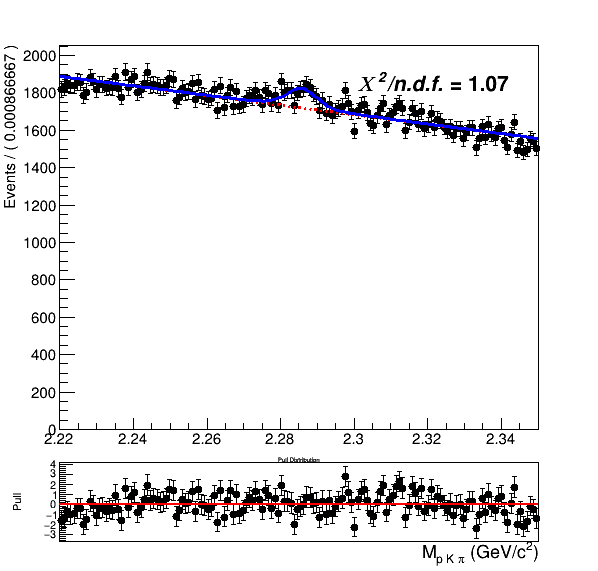
\includegraphics[width=6.4cm]{04-chargedCorrBtoLambda/figs/stream01234Continuum_charged_corrLambdaC_3GaussianInvMfit.png}
   % \caption{Fit of the $\Lambda_c$ invariant mass of on-resonance continuum using the same three gaussian PDF to describe the peak in the signal invariant mass (all nominal cuts applied).}
    \label{fig:charged_corrLambdaC_InvM_continuumMC_3Gaussianfit}
  \end{subfigure}
\caption{$\Lambda_c$ invariant mass fits using five streams. On the left: fit of the $\Lambda_c$ invariant mass of on-resonance continuum using the one Gaussian description (all nominal cuts applied). On the right: fit of the $\Lambda_c$ invariant mass of on-resonance continuum using the same three gaussian PDF to describe the peak in the signal invariant mass (all nominal cuts applied). }
\end{figure} 



%\begin{figure}[h!]
%\centering
%{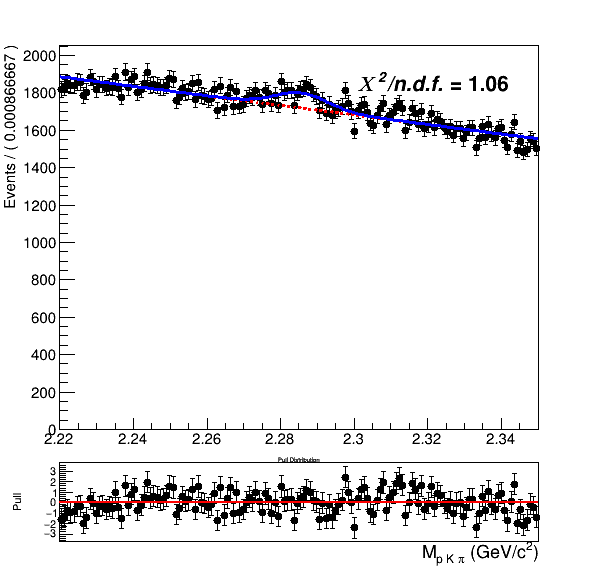
\includegraphics[width=0.4\textwidth]{04-chargedCorrBtoLambda/figs/stream01234Continuum_charged_corrLambdaC_oneGaussianInvMfit.png}}
%\caption{Fit of the $\Lambda_c$ invariant mass of on-resonance continuum using the one Gaussian description (all nominal cuts applied).}
%\label{fig:charged_corrLambdaC_InvM_continuumMC_fit}
%\end{figure}
 
%\begin{figure}[h!]
%\centering
%{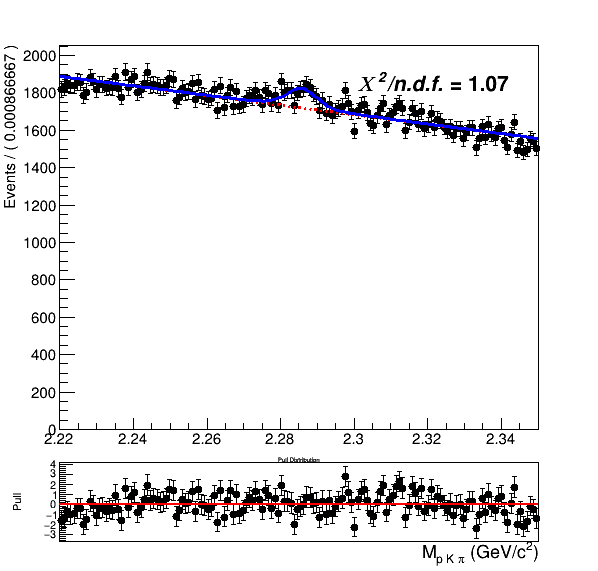
\includegraphics[width=0.4\textwidth]{04-chargedCorrBtoLambda/figs/stream01234Continuum_charged_corrLambdaC_3GaussianInvMfit.png}}
%\caption{Fit of the $\Lambda_c$ invariant mass of on-resonance continuum using the the same three gaussian PDF to describe the peak in the signal invariant mass (all nominal cuts applied).}
%\label{fig:charged_corrLambdaC_InvM_continuumMC_3Gaussianfit}
%\end{figure} 

\begin{figure}[h!]
%\centering
{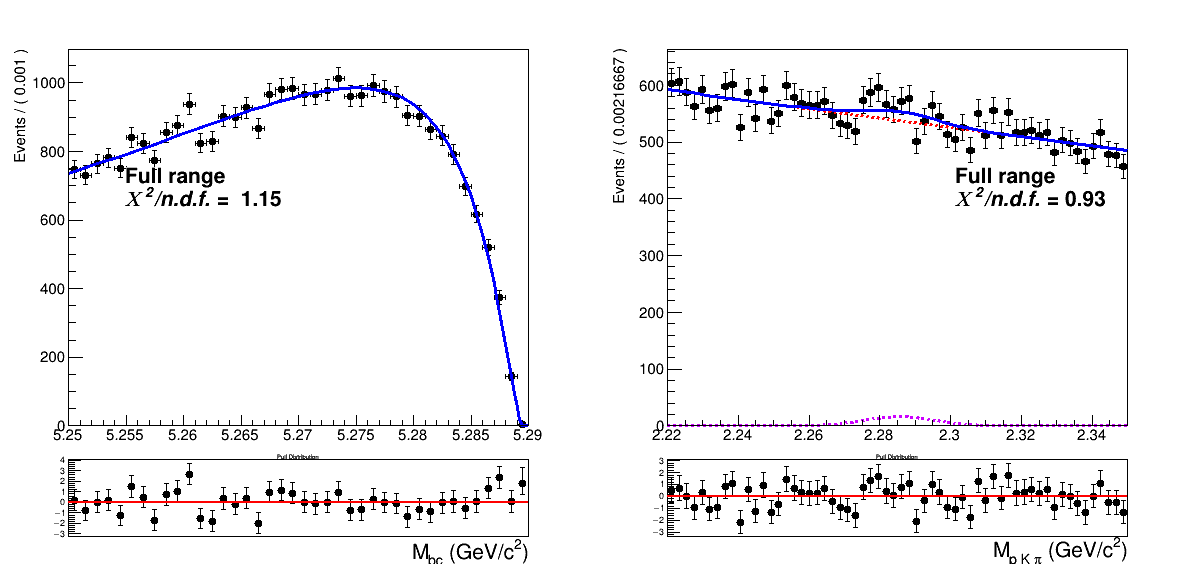
\includegraphics[width=0.85\textwidth]{04-chargedCorrBtoLambda/figs/stream3corrLambddaC_total_continuum_2DFit.png}}
\caption{Two dimensional fit of  continuum events (one stream).}
\label{fig:stream3corrLambddaC_total_continuum_2DFit}
\end{figure}


%\vspace{5 cm}
It was then also investigated to alternatively use the same triple Gaussian PDF (used in Eq. \ref{eq:RecSigEq} for the signal peak) to describe the peak, as it is shown in Fig. \subref{fig:charged_corrLambdaC_InvM_continuumMC_3Gaussianfit}32 . The two descriptions seem to be equivalent. The final fits described in Sec. \ref{2DtotalFit} were performed with the one Gaussian description (keeping all parameters fixed), but it was also tried with the alternative three Gaussian description (with main Gaussian having the  width as free parameter): no significant difference was noticed and the signal yields differ by only about 10$\%$ of the statistical uncertainties. Though, for consistency reasons, on data the second description will be applied. 


\newpage
\subsection{Two dimensional fit}\label{2DtotalFit}

All the already discussed PDFs describing the various categories of events were constructed using five streams. Then an independent stream is used to test if the total PDF enables to extract the signal yield in an unbiased way. In order to test this a total of six fits are performed on six different streams of generic MC. Exemplary, the distributions of stream 0 overlaid by the fitted PDF are depicted in Fig. \ref{fig:stream0_Total2Dfit_charged_corrLambdaC} (see \cref{sec:chargedBtoLamApp} for the projections in signal and sideband regions). 
In all six fits all the shaping parameters are kept fixed, except:
\begin{itemize}
    \item $\sigma_{G1}$: the width of the wider of the three Gaussian functions in $\rho_G(M(p K \pi))$
    \item $\sigma_{CB}$ parameter for the Crystal Ball describing the signal peak in $M_{bc}$
\end{itemize}

In the $M_{bc}$ distribution the $\sigma_{CB}$ parameter for the Crystal Ball describing the generic background is expressed as function of the signal $\sigma_{CB}$  with a ratio fixed from the MC. 
\noindent As for the normalizations, mis-/reconstructed signal events and generic background events are floated in the two dimensional unbinned maximum likelihood fits. 
The continuum background normalization is kept fixed to the value obtained by the off-resonance scaling procedure.  Instead, the normalization of crossfeed background events deserves a special treatment, 
a possible choice would be to express it as a function of the ratio of crossfeed events with respect to the misreconstructed signal events and keep it fixed o the MC value
(this is done then in the fit on all tagged $B$ mesons, i.e. in Sec. \ref{BtagFit}). This would make sense according to the fact that the two categories of events are similar: 
in both cases the $B$ mesons were not correctly reconstructed, either because of missing or wrongly added particles (misreconstructed signal events) or, in the case
of crossfeed events because it was a different one ($B^0$ meson instead of charged one). Since the amount of misreconstructed signal depends on the branching ratio itself, 
this method is not viable. 
Therefore, as for the crossfeed background the normalization of the PDF described in \cref{eq:paramCrossfeedPDF} is parametrized in the form:
\begin{equation}
N_{CrossBkg} P^{CrossBkg}(M_{bc}, M(p K \pi)) = k \cdot N_{B^0} \cdot N_{misRecSig} / N_{sig} \cdot  P^{CrossBkg}(M_{bc}, M(p K \pi)) 
\label{eq:paramCrossfeedNorm}
\end{equation}
\begin{itemize}
\item defining a sort of "probability ratio": $k = \frac{N_{crossfeed }/  N_{B^0}}{N_{misRecSig} /  N_{sig} }$ , where the numerator represents the probability of misreconstructing $B^0$ as $B^+$ events
and the denominator the probability of misreconstructing signal events. This ratio is calculated from MC and will be kept fixed also while fitting data. \\
\item  $N_{B^0} $ is the total number of $B^0$ events in the dataset (MC or data). 
\item $N_{misRecSig}$ is the floated normalization of misreconstructed signal events
\item $ N_{sig}  =  N_{recSig} / \epsilon$ is the total number of signal events expressed as function of the floated normalization of reconstructed signal events and the signal reconstruction efficiency. 
\end{itemize}



\begin{figure}[h!]
%\centering
{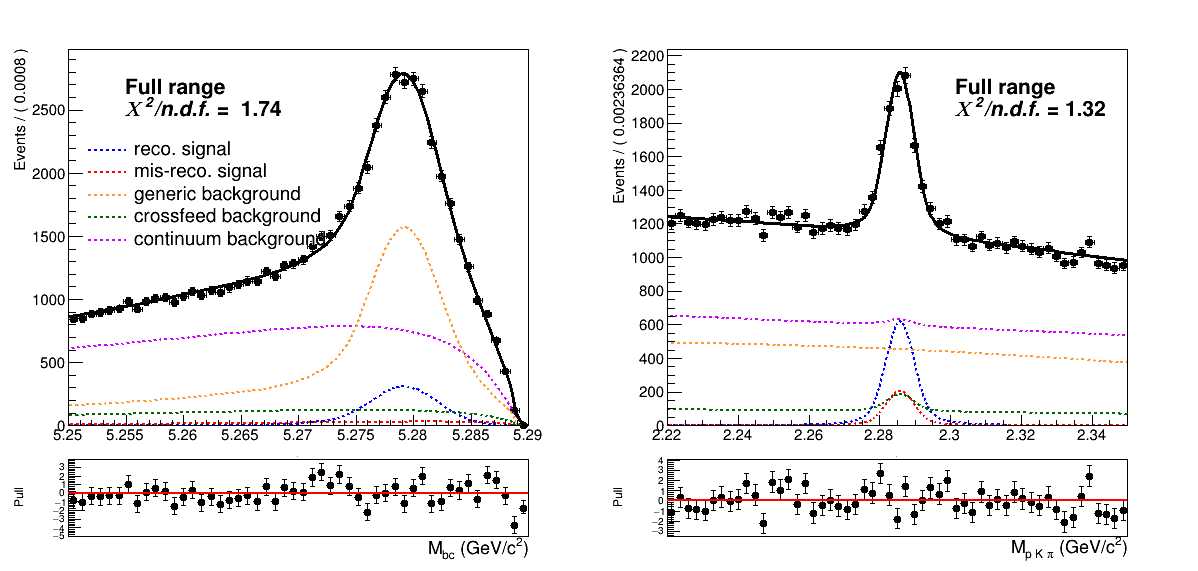
\includegraphics[width=0.85\textwidth]{04-chargedCorrBtoLambda/figs/Total_2DFit_stream0_w_crossfeed_ratio_param.png}}
\caption{Two dimensional fit on stream 0 Monte Carlo simulated data.}
\label{fig:stream0_Total2Dfit_charged_corrLambdaC}
\end{figure}

\begin{figure}[h!]
%\centering
{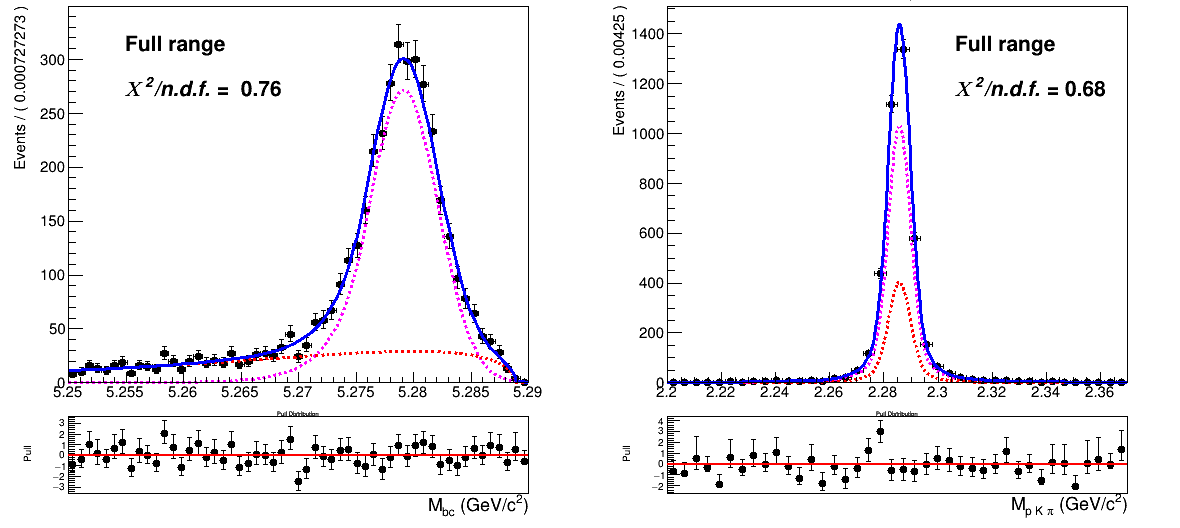
\includegraphics[width=0.75\textwidth]{04-chargedCorrBtoLambda/figs/stream0_TotalSignal_charged_corrLambdaC_2Dfit.png}}
\caption{Two dimensional fit of Total Signal of stream 0 used to extract the expected reconstructed (corresponding to the PDF colored in magenta) and expected misreconstructed yields (corresponding to the PDF colored in red).}
\label{fig:stream0_TotalSignal_charged_corrLambdaC_2Dfit}
\end{figure}

%\noindent The normalizations of    

In Table \ref{tab:SixStreams_chargedCorrLam2Dfits} the signal yields of the fits (\textbf{Reconstructed Signal}) to the two dimensional distributions for the six streams of $B^- \rightarrow \Lambda_c^+$ flavor-correlated decays are listed and compared to the yields obtained from fits of signal distributions of each individual stream. The latter are the "expected" yields of reconstructed signal from a fit to the total signal events in the individual stream as the one plotted on \cref{fig:stream0_TotalSignal_charged_corrLambdaC_2Dfit} where all the parameters of the PDFs described in \cref{eq:RecSigEq} are kept fixed and the corresponding yields are extracted from the fit. 

%Total Signal:
%\begin{table}[ht]
%\centering
%\resizebox{0.8\textwidth}{!}{%
%\setlength{\tabcolsep}{8pt}
%\begin{tabular}{c c c c c c c}

%\toprule
% \hline
%   &	\multicolumn{2}{c}{Reconstructed Signal}  & \multicolumn{2}{c}{Total Signal} &  \\
%     &  fit \hspace{0.5 cm}  & expected  & fit   & MC truth &  \multicolumn{2}{c}{fit - MC truth} \\
% \midrule
% \hline
%stream 0	&	3058 $\pm$ 123 	&	2928 $\pm$ 66	&	4037 $\pm$ 121	&	4061	&  $-24$	&	-0.6$\%$	\\
%stream 1	&	3047 $\pm$ 127	&	2956 $\pm$ 66	&	4098 $\pm$ 126	&	4084	&  14	&	0.3$\%$	\\
%stream 2	&	3032 $\pm$ 126	&	2940 $\pm$ 66	&	4031 $\pm$ 126	&	4138	& -107	&	-2.6$\%$	\\
%stream 3	&	2849 $\pm$ 124	&	2867 $\pm$ 66	&	4140 $\pm$ 123	&	4105	& 35  &   	0.9$\%$	\\
%stream 4	&	3114 $\pm$ 129	&	3031 $\pm$ 67	&	4076 $\pm$ 126	&	4169	&  -93	&	-2.2$\%$	\\
%stream 5	&	2909 $\pm$ 127	&	2816 $\pm$ 65	&	4080 $\pm$ 129	&	4001	&  79	&	2.0$\%$	\\
%\midrule
%\hline
%sum			&	18009		&	17538	&		24462		&	24558	&	-96	&	-0.4$\%$	\\
%\bottomrule
%\hline
%\end{tabular}%
%}%
%\caption{Comparison of fitted and expected signal yields, fitted and truth-matched total signal for six streams of Belle generic MC when fitting the two dimensional distributions of $M_{bc}$ and $M(p K \pi)$.}
%\label{tab:SixStreams_chargedCorrLam2Dfits}
%\end{table}



%Except for stream 3, the fits present slightly higher values of reconstructed signal than expected ones, although always within the 1$\sigma$ uncertainties (as shown in Fig. \ref{fig:RecoSignal_fit-expectedPlot}). 
%Parametrization:\\
%define the probability ratio:
%\begin{equation}
%k = \frac{N_{crossfeed}/N_{B^0}}{N_{misrecSig}/N_{sig}}
%\end{equation}
%,  where $N_{sig} = N_{recSig}/\epsilon$\\
%$N_{crossfeed}P^{crossfeed}(M_{bc}, M(p K \pi)) = k \cdot N_{B^0}  \cdot N_{misrecSig}/N_{sig} \cdot P^{crossfeed}(M_{bc}, M(p K \pi))$
%\newline
%$\epsilon$: signal reconstruction efficiency
%%%%%%%%%%%%%%%%%%%%%%%%%%%%%
%\textbf{After crossfeed ratio parametrization}:

\begin{table}[H]
\centering
\resizebox{0.8\textwidth}{!}{%
\setlength{\tabcolsep}{8pt}
\begin{tabular}{c c c c c c c}

\toprule
 \hline
   &	\multicolumn{2}{c}{Reconstructed Signal}  & \multicolumn{2}{c}{Total Signal} &  \\
     &  fit \hspace{0.5 cm}  & expected  & fit   & MC truth &  \multicolumn{2}{c}{fit - MC truth} \\
 \midrule
 \hline
stream 0	&	3072 $\pm$ 113 	&	2928 $\pm$ 66	&	4037 $\pm$ 121	&	4061	&  -24	&	-0.6$\%$	\\
stream 1	&	2919 $\pm$ 115	&	2956 $\pm$ 66	&	4098 $\pm$ 126	&	4084	&  14	&	0.3$\%$	\\
stream 2	&	2627 $\pm$ 119	&	2940 $\pm$ 66	&	4031 $\pm$ 126	&	4138	& -107	&	-2.6$\%$	\\
stream 3	&	2865 $\pm$ 111	&	2850 $\pm$ 66	&	4140 $\pm$ 123	&	4105	& 35  &   	0.9$\%$	\\
stream 4	&	3328 $\pm$ 119	&	3046 $\pm$ 67	&	4076 $\pm$ 126	&	4176	&  -100	&	-2.2$\%$	\\
stream 5	&	2959 $\pm$ 114	&	2816 $\pm$ 65	&	4080 $\pm$ 129	&	4001	&  79	&	2.0$\%$	\\
\midrule
\hline
sum			&	17770		&	17538	&		24462		&	24565	&	-103	&	-0.4$\%$	\\
\bottomrule
\hline
\end{tabular}%
}%
\caption{Comparison of fitted and expected signal yields, fitted and truth-matched total signal for six streams of Belle generic MC when fitting the two dimensional distributions of $M_{bc}$ and $M(p K \pi)$.}
\label{tab:SixStreams_chargedCorrLam2Dfits}
\end{table}


\noindent  The table also reports the fitted and truth-matched number of total signal (sum of reconstructed and misreconstructed signal) events. 
One can notice that, despite the deviations of total signal events being within statistical uncertainties, the results for reconstructed signal (first column)
show fluctuations which exceed the statistical uncertainties, especially in case of stream 2 and 4 (see also \cref{fig:RecoSignal_fit-expectedPlot} and \cref{fig:charged_corrLambdaRecoSignal_deviations}) 
One can notice also an overall tendency towards higher values for the signal yields (the sum is about 2$\sigma^{stat.}$ away from the sum computed for the expected yields).%, which indicates that this sum doesn't present biases. Nevertheless the fact that the reconstructed signal is not fluctuating around zero can be seen as an evidence of a small bias. Fig. \ref{fig:RecoSignal_deviations} shows the differences between fitted and expected values of reconstructed signal with associated uncertainties (calculated as sum of quadrature of both uncertainties on the results from the fits and the expected values). The performed linear fit shows that, taken together, the six fits present an overall, small but not negligible, bias, which has to  be taken into account while fitting the data.


\begin{figure}[H]
%\centering
{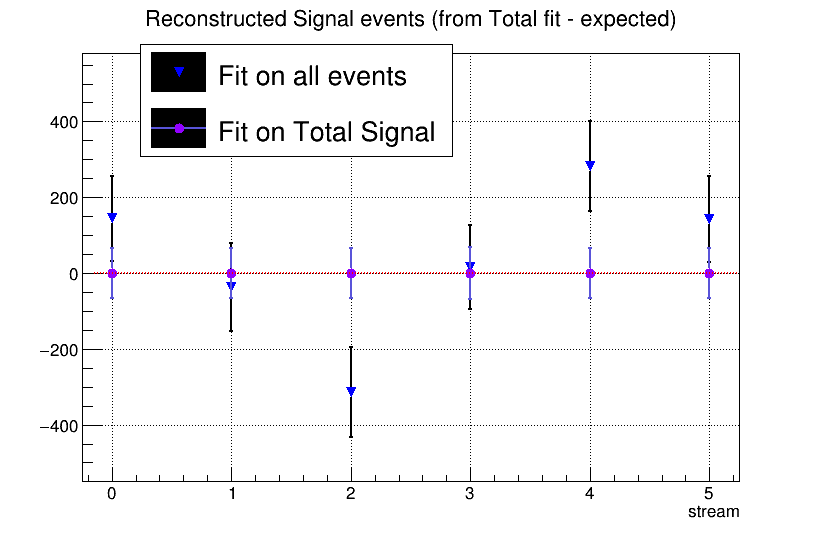
\includegraphics[width=0.65\textwidth]{04-chargedCorrBtoLambda/figs/RecoSignal_fit_chargedCorrLambdaC_afterCrossfeedRatioParam.png}}
\caption{Differences between results from the fits and "expected" values for signal yields as reported in the first columns on Table\ref{tab:SixStreams_chargedCorrLam2Dfits} .}
\label{fig:RecoSignal_fit-expectedPlot}
\end{figure}

\begin{figure}[h]
%\centering
{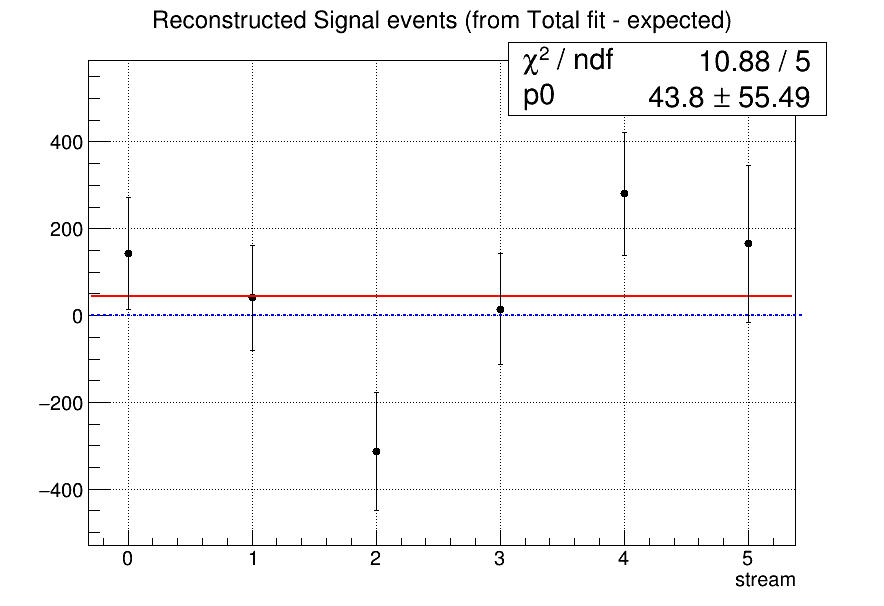
\includegraphics[width=0.63\textwidth]{04-chargedCorrBtoLambda/figs/RecoSignal_streams_fittedPoints_chargedCorrLambdaC_w_CrossfeedRatio_param.png}}
\caption{Fitted-expected subtracted values for reconstructed signal yields with associated uncertainties summed in quadrature.}
\label{fig:charged_corrLambdaRecoSignal_deviations}
\end{figure}


\noindent Additionally, one can investigate the behaviour for different signal-to-background ratio. Thus, a second test of the fit model is performed. 
Using the six independent streams the  amount of total signal is varied between 25$\%$ and 150$\%$ of the nominal values.% The amount of background varies according to poissonian fluctuations, as it is taken from four independent streams. 
\noindent  The plot in Fig. \ref{fig:LinearityTest_chargedCorrLambdaC} shows the values of reconstructed signal obtained in the total fits versus those expected by the fits on total signal events. 
One can see that the values distribute according to a linear dependence. In \cref{fig:LinearityTest_BR_chargedCorrLambdaC} the linearity test is expressed in terms of $\mathcal{B}(B^+ \rightarrow \bar{\Lambda}_c^- X)$ instead. % The linear fit suggests a compatibility with a 1:1 relation: the red and the blue dotted lines don't overlap, but the values of the fitted line are compatible within the uncertainties with the identity line. Though also in this second test we see a slight tendency of overshooting the expected values.   

\begin{figure}[H]
%\centering
{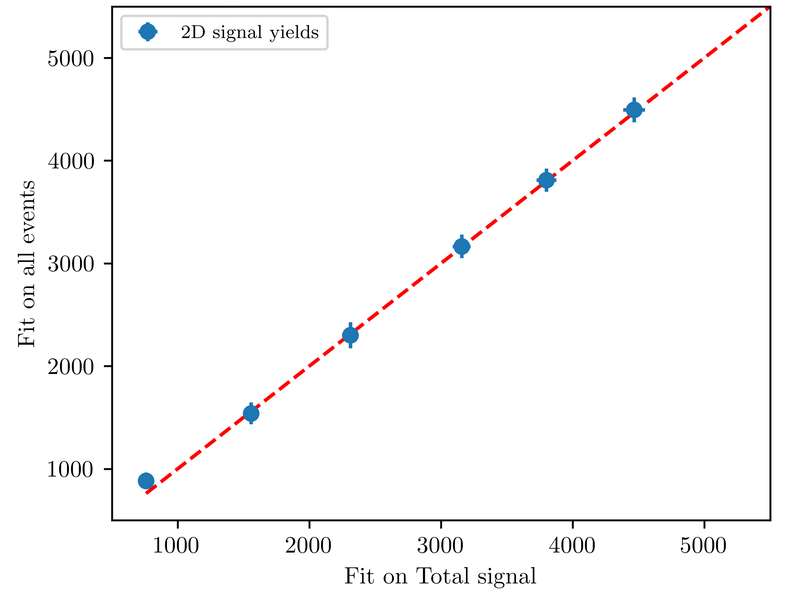
\includegraphics[width=0.75\textwidth]{04-chargedCorrBtoLambda/figs/ReconstructedSignal_Fit_LinearityTest_chargedCorrLambdaC.png}}
\caption{Linearity test: on the x-axis the obtained reconstructed signal yields from fits on different amounts of total signal; on y-axis the yields of reconstructed signal obtained fitting all events
 (as in Fig. \ref{fig:stream0_Total2Dfit_charged_corrLambdaC}). The dashed red line represents the 1:1 linear dependence.}
\label{fig:LinearityTest_chargedCorrLambdaC}
\end{figure}



\begin{figure}[H]  
  %\centering
{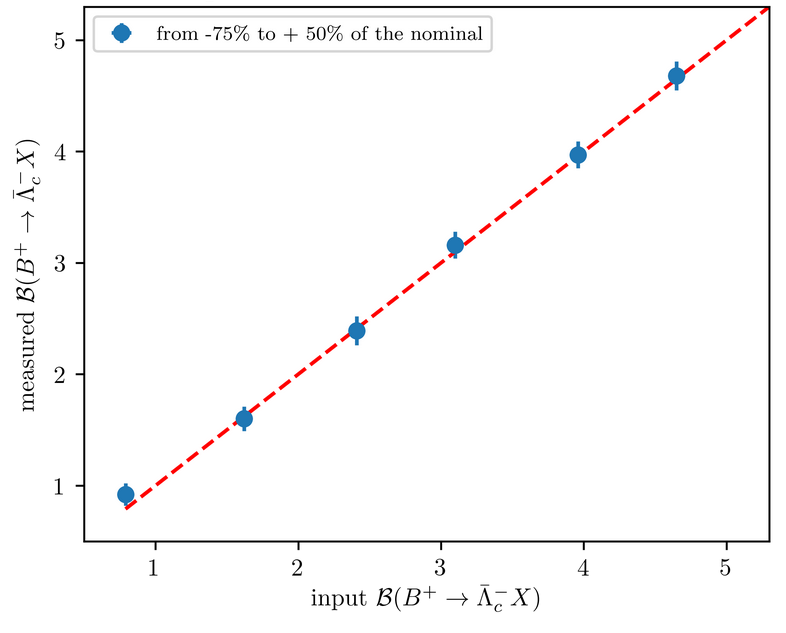
\includegraphics[width=0.75\textwidth]{04-chargedCorrBtoLambda/figs/chargedCorrLambdaC_BR_linearity.png}}
\caption{Linearity test: on the x-axis the input branching ratio value corresponding to the signal yields displayed on the x-axis in \cref{fig:LinearityTest_chargedCorrLambdaC}; 
on y-axis the measured branching fraction values corresponding to the signal yields of reconstructed signal displayed on the y-axis in \cref{fig:LinearityTest_chargedCorrLambdaC}.}
\label{fig:LinearityTest_BR_chargedCorrLambdaC}
\end{figure}

\noindent For the fit model also toy MC pseudo-experiments were
performed in order to confirm the behavior of the fit setup.  With toy MC experiments the yields, errors and the pulls of the fit are studied  by generating our own pseudo-datasets, according to the MC (see plots in the next page). 
 $3\times10^3$ pseudo-datasets are constructed, where each dataset was generated with the expected amount of events, distributed according to the Poisson distribution. Then the composition of each toy pseudo-experiment is fitted as if they were data, and the pull-value distributions of the fit results are calculated.
 The pulls distributions are centered at zero, indicating there's no significant bias in the fitted yields/parameters.
\newpage


\begin{figure}[H]
  \begin{subfigure}{14.5cm}
    \centering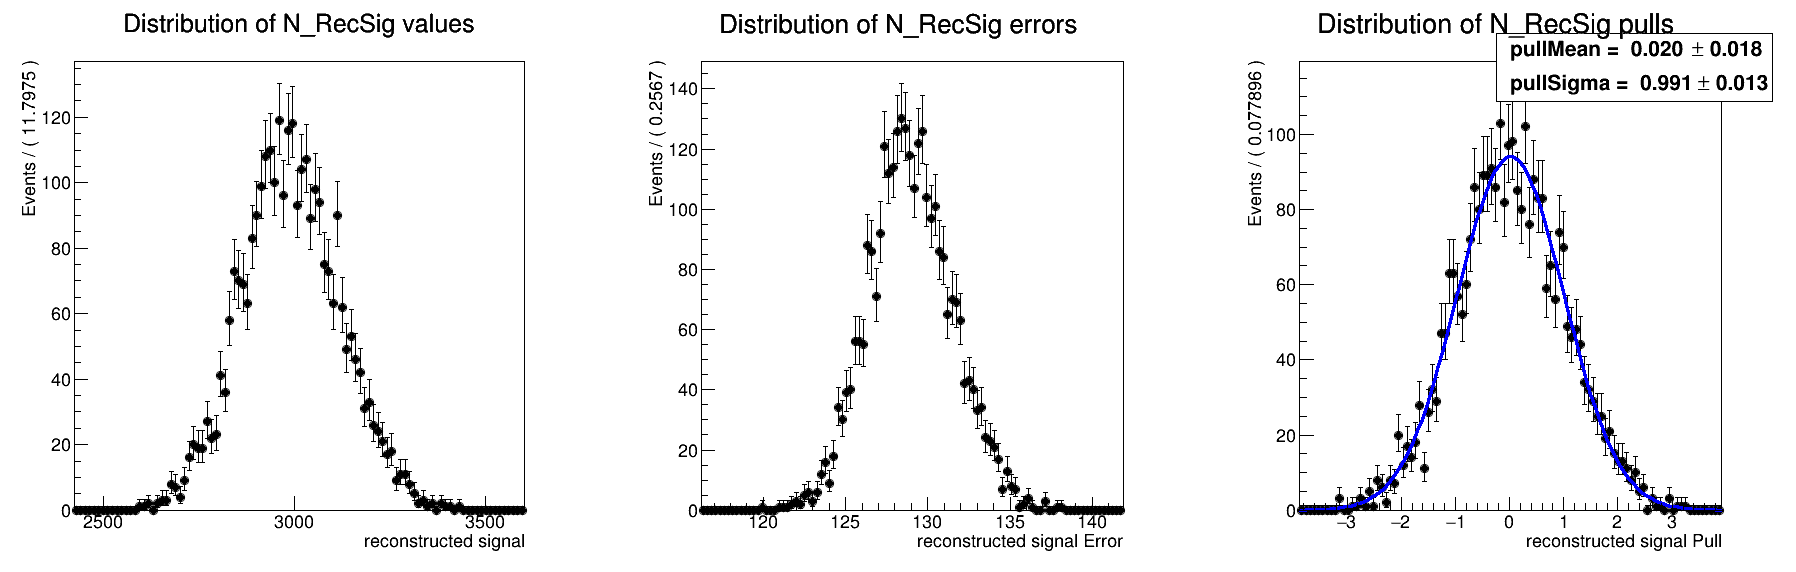
\includegraphics[width=13.8cm]{04-chargedCorrBtoLambda/figs/NrecSig_mcstudy.png}
   % \caption{Fit on $M(p K \pi)$ in the region $5.25 < M_{bc} < 5.258$ GeV/c$^2$.  }
   % \label{fig:CrossfeedMbcRegionsInvMpeak1}
  \end{subfigure}
  \begin{subfigure}{14.5cm}
    \centering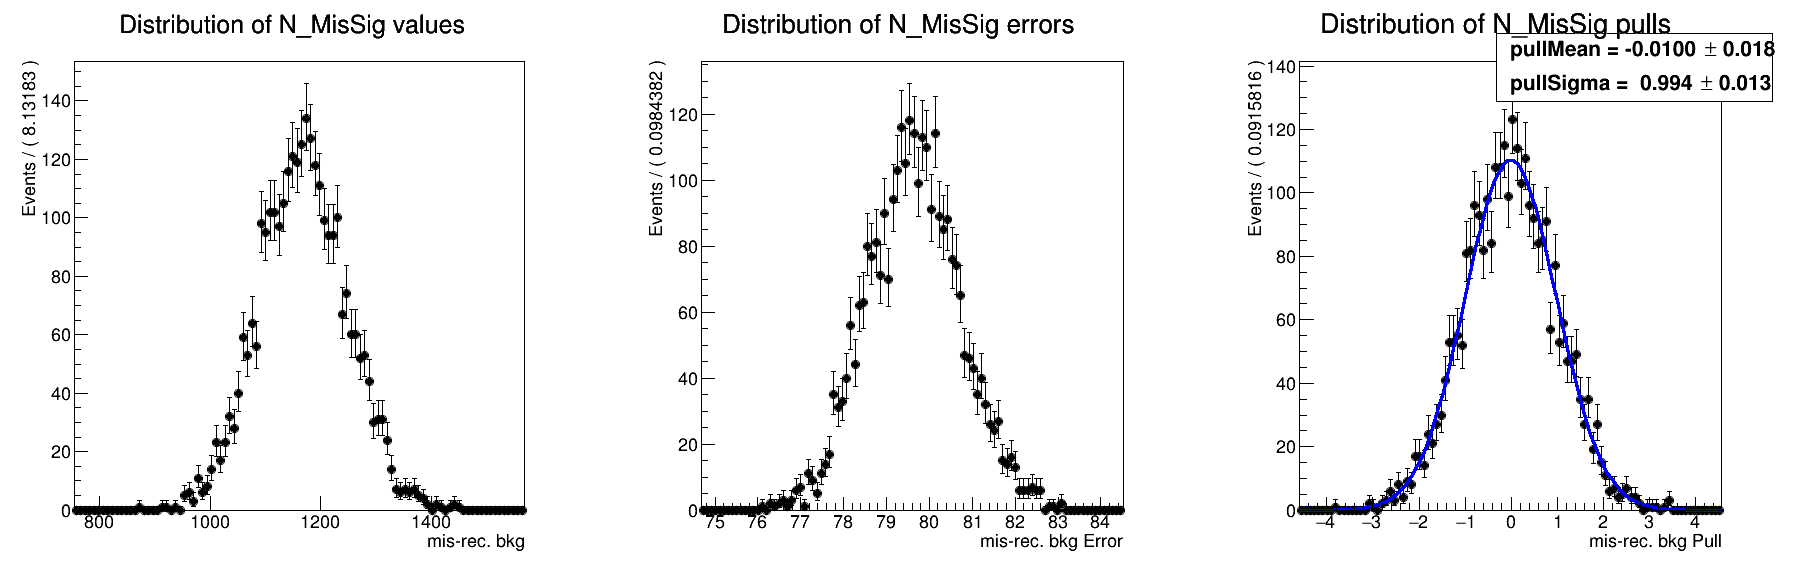
\includegraphics[width=13.8cm]{04-chargedCorrBtoLambda/figs/NmisSig_mcstudy.png}
  \end{subfigure}
 
  \begin{subfigure}{14.5cm}
    \centering\includegraphics[width=13.8cm]{04-chargedCorrBtoLambda/figs/N_Generic_mcstudy.png}
  \end{subfigure}
  \begin{subfigure}{14.5cm}
    \centering\includegraphics[width=13.8cm]{04-chargedCorrBtoLambda/figs/sigmaCB1_mcstudy.png}
  \end{subfigure}
  \begin{subfigure}{14.5cm}
    \centering\includegraphics[width=13.8cm]{04-chargedCorrBtoLambda/figs/InvMsigma_mcstudy.png}
    %\label{fig:CrossfeedMbcRegionsInvMpeak5}
  \end{subfigure}
  %\label{fig:CrossfeedMbcRegionsInvMpeak}
  \caption{Toy MC study plots for the two dimensional fit model}
\end{figure}

\newpage


\subsection{Probability Density Functions (PDFs) for the $B_{tag}$}
The $M_{bc}$ distribution of the tagged  $B$ mesons is fitted with a Crystal Ball as for the "peaking" component and the "flat" component is fitted with a Novosibirsk function (Fig. \ref{fig:stream0_chargedBtag_Total_Signal_fit_restrictedRange}). 
The crossfeed background, consisting of neutral $B$ mesons tagged as charged $B$, is fitted instead with a sum of a Novosibirsk and an asymmetric Gaussian PDF (Fig. \ref{fig:NeutralCrossfeed_stream0_corrLambdaC_chargedBtagFit}). 
Both fits shows a $\chi^2 /n.d.f.$ considerably higher than one and pulls exceeding 3$\sigma$ deviation in some regions, but the systematics represented by this is negligible compared to other sources of systematic uncertainties and statistical uncertainties in the two dimensional fit.


\begin{figure}[h!]
\centering
{\includegraphics[width=0.40\textwidth]{04-chargedCorrBtoLambda/figs/stream0_chargedBtag_Total_Signal_fit_restrictedRange.png}}
\caption{Fitted distribution of tagged charged $B$ mesons: reconstructed signal events are described by the blue dotted PDF, the misreconstructed with a Novosibirsk function (red dotted). }
\label{fig:stream0_chargedBtag_Total_Signal_fit_restrictedRange}
\end{figure}

\begin{figure}[h!]
\centering
{\includegraphics[width=0.40\textwidth]{04-chargedCorrBtoLambda/figs/NeutralCrossfeed_stream0_corrLambdaC_chargedBtagFit.png}}
\caption{Crossfeed distribution fitted with a sum of Novosibirsk (red) and asymmetric Gaussian PDF (magenta)}
\label{fig:NeutralCrossfeed_stream0_corrLambdaC_chargedBtagFit}
\end{figure}

\newpage

\noindent  As for the continuum background, a similar procedure as the one described already for the two dimensional fit was adopted:

\begin{itemize}
    \item first the off-resonance sample is scaled accordingly
    \item the ratio between the scaled off-resonance and the on-resonance in MC is calculated in each bin (see Fig.\ref{fig:stream0_chargedBtag_off-on_resonance})
    \item the bin-correction is applied on an independent stream and the scaled and bin-corrected $M_{bc}$ distribution is compared with the on-resonance distribution as shown in Fig.\ref{fig:bin_corrected_stream1_off-resonance_on_stream0_on-resonance}
\end{itemize}
\vspace{0.5cm}
As for the $B_{tag}$ continuum background the statistics is much larger than in the 2D sample, there's no need to remove the continuum suppression cut on the off-resonance sample. 

\begin{figure}[H]
 \centering
\subcaptionbox{\label{fig:stream0_chargedBtag_off-on_resonance}}
{\includegraphics[width=.45\textwidth]{04-chargedCorrBtoLambda/figs/stream0_chargedBtag_off-on_resonance.png}}
\subcaptionbox{\label{fig:bin_corrected_stream1_off-resonance_on_stream0_on-resonance}}
{\includegraphics[width=.44\textwidth]{04-chargedCorrBtoLambda/figs/bin_corrected_stream1_off-resonance_on_stream0_on-resonance.png}} 
\caption{On the left: $M_{bc}$ distributions of the MC off-resonance sample and the MC continuum sample with applied continuum suppression. On the right: $M_{bc}$ distributions of the corrected scaled MC off-resonance and on-resonance MC continuum.}
\end{figure}



\newpage
\subsection{ $B_{tag}$ fit}\label{BtagFit}
An independent Monte Carlo stream was used to test the total fit model on tagged $B$ meson candidates.
As in the 2D fit, the parameter for the width, $\sigma_{CB}$, of the Crystal Ball is floated and the ratio between expected crossfeed background events and  misreconstructed signal events is fixed from the MC. 
The Novosibirsk function describing the misreconstructed signal is also not fully constrained: the parameter describing the tail is free. To avoid introducing significant systematic
uncertainties in the fit deriving from the $M_{bc}$ endpoint region, where one has a smearing effect due to variations of the
beam energy at the MeV level, the range for the fit is restricted to values betweeen 5.250 and 5.287 GeV/c$^2$.
Yields for the reconstructed and misreconstructed signal are obtained from the fit:\\
\vspace{0.25 cm}

\begin{tabular}{ |p{2.5cm}||p{4.2cm}|  }
 \hline
 NrecSig  & 4.2681$\cdot$10 $^6 \pm$ 5871\\
 NmisSig &  5.8787$\cdot$10 $^6 \pm$ 5128 \\
 \hline
\end{tabular}

\vspace{0.5 cm}
 The Total Signal (the sum  NrecSig+NmisSig) is 10146748 $\pm$ 4380 (to be compared with 10158571 from the Monte Carlo). This reflects a $\sim 2.5\sigma$ discrepancy between the true MC value and the result from the fit. This can produce some systematic effect, but the relative error is at the $\sim$ \textperthousand level. This is still negligible compared to the systematic uncertainity corresponding to the the ${N_{tag}}$ determination, and furthermore in the branching fraction calculation it is also negligible compared to the statistical uncertainity on the extracted yields from the two dimensional fit.
 
To check the stability of the fit model a toy MC study was performed with  $3\times10^3$ pseudo-datasets (as it was done for the two-dimensional fit model). No evidence for possible biases in the reconstructed signal yields was found (see \cref{fig:NrecSignalchargedCorrBtag_mcstudy}).

\begin{figure}[h!]
\centering
{\includegraphics[width=0.50\textwidth]{04-chargedCorrBtoLambda/figs/chargedCorrLambdaC_BtagFit.png}}
\caption{Total fit of tagged $B$ mesons on Monte Carlo simulated data.}
\label{fig:chargedCorrLambdaC_BtagFit}
\end{figure}
\vspace{1.5cm} 


  \begin{figure}[H]
\centering
{\centering\includegraphics[width=14cm]{04-chargedCorrBtoLambda/figs/NrecSigBtag_mcstudy.png}}
 \caption{Plots showing distributions of the fitted signal yields, errors and the pull distribution of
all pseudo-fits. (see Appendix \ref{sec:chargedBtoLamApp} for the other free parameters' results)}
  \label{fig:NrecSignalchargedCorrBtag_mcstudy}
  \end{figure}


\subsection{$\Lambda_c$ and FEI efficiency}

The efficiency in reconstructing the ${\Lambda_c}$ baryon after correctly tagging the charged $B$ meson, can be estimated from Monte Carlo simulated data as the fraction of correctly reconstructed signal events that have a correctly reconstructed $B_{tag}$ companion, i.e.: 

\begin{equation}
    \frac{N_{recSig}(B_{tag}, \Lambda_c)}{N_{recSig}(B_{tag}^{sig})}
\end{equation}

\vspace{0.5cm}

\noindent where $N_{recSig}(B_{tag}, \Lambda_c))$ are the yields of reconstructed signal from the two dimensional fits (reported in Table \ref{tab:SixStreams_chargedCorrLam2Dfits} ) and  $N_{recSig}(B_{tag}^{sig})$ are the yields of correctly reconstructed signal in a fit of $B$ mesons tagged in events where one of the two mesons decayed hadronically and inclusively into a ${\Lambda_c}$ baryon (see Fig \ref{fig:sixstreams_chargedBtagSignal_fit}). 
To minimize statistical uncertainties, in the efficiency calculation the results from all the two dimensional fits were used and six streams of $B_{tag}$ candidates reconstructed in signal events were used for the $M_{bc}$ shown below.

\begin{figure}[h!]
%\centering
{\includegraphics[width=0.40\textwidth]{04-chargedCorrBtoLambda/figs/chargedBtag_corrLambdaC_TotalSignalBtag_fit.png}}
\caption{Fit of tagged $B$ mesons in the "signal events" sample}
\label{fig:sixstreams_chargedBtagSignal_fit}
\end{figure}


\vspace{0.5 cm}
From this and the results listed in sec. \ref{2DtotalFit} 
the efficiency to reconstruct ${\Lambda_c}$ is obtained : \\

$\epsilon_{\Lambda_c} = \frac{NrecSig(B_{tag}, \Lambda_c) }{NrecSig(N_{recSig}(B_{tag}} = 44.83 \pm 0.32 \%$  %\hspace{1cm} (KID efficiency corrected value for data: 38.2 $\%$)
\vspace{0.2 cm}

The yields from the fit shown in  (Fig. \ref{fig:sixstreams_chargedBtagSignal_fit}) can be used also to calculate the FEI tag-side efficiency for signal events, i.e. the efficiency to tag the $B$ meson accompanying a $B_{sig}$ decaying into a $\Lambda_c $ on the signal side.
Whereas results from the fit  of charged $B_{tag}$ shown in Fig. \ref{fig:stream0_chargedBtag_Total_Signal_fit_restrictedRange} can be used to calculate the hadronic tag-side efficiency in the generic $B^+B^-$ events case.

The ratio between the two efficiencies is calculated: 
 $\frac{\epsilon^{+}_{FEI,  sig}}{\epsilon^{+}_{FEI}} = 0.908 \pm 0.017 $ \\\vspace{0.4 cm}
\newpage

\subsection{Studies of Systematic Effects}

In Table \ref{tab:systematics:ChargedCorr} the systematic uncertainties of the various considered sources are summarized. The full estimate of the systematic uncertainty is summed up in quadrature and applied to the result in Section \ref{BrValue}
Their individual calculation is outlined in the subsequent subsections.

\begin{table}[h]
\centering
\resizebox{0.5\textwidth}{!}{%
\begin{tabular}{lS}
\hline
source              & $\%$  \\
\hline
Continuum modeling      &  0.07 \\
Crossfeed PDFs      &  0.07 \\
Crossfeed fraction      &  0.06 \\
2DFit crossfeed normalization & 0.02 \\
2DFit crossfeed peaking fraction & 0.09* \\
$\epsilon^{+}_{FEI,  sig}/\epsilon^{+}_{FEI}$ & 0.06 \\
$\epsilon_{\Lambda_c}$ & 0.02 \\
Fit bias        & 0.06 \\
PID                & 0.05 \\
Tracking efficiency  & 0.01 \\
\hline
Total                         &   0.20   \\
\hline
\end{tabular}%
}%
\caption{Systematic uncertainties in the determination of the  $B^+ \rightarrow \bar{\Lambda}_c^- X$ branching fraction in \si{\percent}.}
\label{tab:systematics:ChargedCorr}
\end{table}

* this represents the dominant uncertainty, but in \cref{sec:PeakingCrossBkg} it will be explained how it can be possibly reduced.


\subsection{Continuum background modeling}\label{sec:chargedCorr_continuumBkgSys}

Regarding this source of systematics, one has two take into account two different types. 
First of all the statistical uncertainties, which are reflected in the uncertainties on the PDF parameters. To estimate this type of uncertainty two-dimensional fits with varied parameters' values by their uncertainties (a fit with $+$err and $-$err) were performed. Whereas, the estimation of statistical uncertainty in the case of the $B_{tag}$ should be estimated in principle varying each bin content of its error. On first approximation this is equivalent to vary the nominal number of events described with the histogram PDF by Poissonian variation. 
Exemplary, fits used to estimate the impact of these uncertainties are shown here in Figures \ref{fig:Signal_window_Total_2DFit_stream5_free_sigmas_ContinuumSys_Plus} - \ref{fig:stream1_chargedBtag_Total_fit_ContinuumSys_Plus}.
The yields obtained from those fits for benchmark stream5 results are then compared with the ones already reported previously and a mean deviation value is obtained for both the two-dimensional fit and the $B_{tag}$ fit.

 

\begin{figure}[h!]
%\centering
{\includegraphics[width=0.75\textwidth]{04-chargedCorrBtoLambda/figs/Signal_window_Total_2DFit_stream5_free_sigmas_Plus.png}}
\caption{Signal window projections of a two dimensional fit on Monte Carlo simulated data where the shaping parameters were varied of their uncertainties.}
\label{fig:Signal_window_Total_2DFit_stream5_free_sigmas_ContinuumSys_Plus}
\end{figure}

\begin{figure}[h]
%\centering
{\includegraphics[width=0.5\textwidth]{04-chargedCorrBtoLambda/figs/stream1_chargedBtag_Total_fit_ContinuumSys_Plus.png}}
\caption{Fit of tagged $B$ meson candidates on Monte Carlo simulated data where the amount of continuum was varied according to poissonian fluctuations.}
\label{fig:stream1_chargedBtag_Total_fit_ContinuumSys_Plus}
\end{figure}

\begin{table}[H]
\begin{tabular}{ |p{2.5cm}||p{2cm}| p{2cm}|  p{2cm}|}
\hline
    Fit    &  $- \sigma$ &  $+ \sigma$ & $ \pm \bar{\sigma}$\\
 \hline
 2D        &     87  & 53  & 70 \\
 $B_{tag}$ &  10218 &  10620 & 10419 \\
 \hline
\end{tabular}
\caption{Offsets on the signal yields obtained in the two dimensional and $B_{tag}$ fit and mean deviations reported in the last column.}
\end{table}
\vspace{0.2 cm}
\noindent The estimated systematic uncertainty on Br value from this source is 0.07$\%$.

The other type of systematic uncertainty in modeling the continuum is originated by the continuum suppression cut having a slightly different efficiency on data (as a consequence of the shift in off-resonance MC and data visible in the the $foxWolframR2$ distribution in Fig. \ref{fig:R2_MC-Data_off_resonance_distributions}). As already discussed, it originates a possible  discrepancy of about 2.25$\%$ in continuum background events in the two dimensional fit (and only 1.25$\%$  in the $B_{tag}$ fit). The statistical uncertainty on this fraction of events can also be taken into account as systematics. Being the number of events in the off-resonance data sample without the continuum suppression applied is very small (less than $10^4$ in the two dimensional fit and about 18500 in the $B_{tag}$ fit), the uncertainty in the mentioned fraction of events is negligible compared to the statistical uncertainty on the on-resonance continuum background events in MC: it would account for 0.002$\%$ on the BR value. Therefore, this second source of uncertainty is not taken into account.
There would be also a third of systematic uncertainty given by potential difference in the on-/off-resonance correction between data and MC, but there's no way one can estimate it properly.
 %0.2$\%$ compared to 0.6$\%$relative


\subsection{Crossfeed background modeling}\label{sec:chargedCorrCrossfeedPDF}

Since also the shapes of the PDFs decribing the crossfeed background are fully fixed to the ones determined with the limited Monte Carlo statistics, also their statistical uncertainties need to be taken into account as possible source of systematics. 
The procedure to estimate this source of systematic uncertainty is the same described in the previous section regarding the continuum background. In the table below the signal yields' offsets are listed changing the parameters within their uncertainties, 
and the mean offsets value used to calculate the expected uncertainty on the BR value. The resulting absolute systematic uncertainty is about 0.07$\%$ on the BR value.

 \vspace{0.25 cm}
\begin{table}[H]
\begin{tabular}{ |p{2.5cm}||p{2cm}| p{2cm}|  p{2cm}|}
\hline
    Fit    &  $- \sigma$ &  $+ \sigma$ & $ \pm \bar{\sigma}$\\
 \hline
 2D        &     51  & 90  & 71 \\
 $B_{tag}$ &  5400 &  5700 & 5550 \\
 \hline
\end{tabular}
\caption{Offsets on the signal yields obtained varying the parameters of crossfeed background PDFs within their uncertainties in the two dimensional and $B_{tag}$ fit and mean deviations reported in the last column.}
\end{table}
 \vspace{0.25 cm}

\subsection{Crossfeed ratio}\label{sec:chargedCorrCrossfeedSys}

The crossfeed/misreconstructed signal "probability ratio" ($k = \frac{N_{crossfeed }/  N_{B^0}}{N_{misRecSig} /  N_{sig} }$) defined in \cref{eq:paramCrossfeedNorm} is kept fixed in the two-dimensional fit and the ratio bewteen crossfeed and misreconstructed events is also kept fixed in the $B_{tag}$ fit to the values found in MC. 
This choice was made according to the fact that the two categories of events are similar: in both cases the $B$ mesons were not correctly reconstructed, either because of missing or wrongly added partilces (misreconstructed signal events) or, in the case of crossfeed events because the tagged $B$ meson was not the required one ($B^0$ meson instead of a $B^{+/-}$ meson). 
The ratio between these two categories of events is therefore expected to be very similar in MC and data, though there's no guarantee that the efficiency to reconstruct them is the same in data
in data and consequently the above mentioned ratios could be differ on data. Unfortunately there's no direct way to have an estimate of the possible discrepancy for them.\\  
In \cite{gelb_moritz_2018_21546} (and previously in \cite{schwab_judith_2017_21422}) it was found that there's a substantial difference in terms of tagging efficiency for FEI applied on Monte Carlo and on Belle data, being the discrepancy around $\sim$ 20$\%$. We can assume that the efficiency for the two categories of events on data will both differ of that value and the ratio of the events being the same MC value, but in absence of any other method to estimate the uncertainty on it one can consider a maximal discrepancy of 20$\%$ between Monte Carlo and data to study the impact on the yields\footnote{This method was also validated with the control decay sample and the originated uncertainty is well within the PDG reported ones.}. 

 Therefore, for the two-dimensional fit the ratio $k $ was artificially varied of $\pm$20$\%$, whereas in the case of the $B_{tag}$ fit the number of crossfeed events were varied artificially in order to have $\pm$20$\%$ different ratio, keeping the previosuly determined Monte Carlo ratio fixed.  
 \vspace{0.25 cm}
\begin{table}[H]
\begin{tabular}{ |p{2.5cm}||p{2cm}| p{2cm}|  p{2cm}|}
\hline
    Fit    &  $- \sigma$ &  $+ \sigma$ & $ \pm \bar{\sigma}$\\
 \hline
 2D        &     54  & 69  & 61 \\
 $B_{tag}$ &  2807 &  3940 & 3374 \\
 \hline
\end{tabular}
\caption{Offsets on the signal yields obtained varying of $\pm$20$\%$ the $k$ ratio in the two dimensional and the ratio of crossfeed/misreconstructed events in the $B_{tag}$ fit and mean deviations reported in the last column.}
\end{table}
 \vspace{0.25 cm}
The estimated systematic uncertainty on Br value from this source is 0.06$\%$. 
\vspace{0.5 cm}

\subsection{Parametrization of crossfeed normalization in the 2D fit}\label{sec:CrossBkgNormalization}

In the previous section, regarding the two-dimensional fit, the uncertainties arising from the fixed "probability ratio" $k$ were investigated. Besides those, one can consider also 
systematic uncertainties of statistical nature deriving from \cref{eq:paramCrossfeedNorm}, were only the number of mis-/reconstructed signal events ($N_{recSig}$/$N_{misrecSig}$) are floated and fitted by the 2D fit.
As already done in the case of continuum and crossfeed PDFs, this type of systematics is estimated repeating the 2D fit varying the parameters by their uncertainties.
This source of systematics originates an uncertainty of 0.02$\%$ on the Br value.


\subsection{Crossfeed peaking fraction in the 2D fit}\label{sec:PeakingCrossBkg}

When discussing the crossfed background modeling (see \cref{fig:5streams_Crossfeed_charged_corrLambdaC_2Dfit}), it was said that among the crossfeed background events 
there are also those that belong to $B^0 \rightarrow \Lambda_c$ decays, which peak in the $ \Lambda_c$ mass. The branching ratio of those decays is also still measured with poor accuracy 
(e.g. $\mathcal{B}(\bar{B}^0 \rightarrow \bar{\Lambda}_c^+ X) = (5.0^{+2.1}_{-1.5})\%$ ), therefore the amount of crossfeed events peaking in $M(p K \pi)$ on data can differ significantly from MC.
To estimate this source of systematics the amount of peaking events was varied in order to cover the uncertainties in the branching fraction mentioned above and repeating the two-dimensional fit.   

\begin{figure}[H]
  \begin{subfigure}{7cm}
    \centering\includegraphics[width=6.5cm]{04-chargedCorrBtoLambda/figs/Plus.png}
   
    \label{fig:neutralCrossfeedInvMpeakPlus}
  \end{subfigure}
  \begin{subfigure}{7.2cm}
    \centering\includegraphics[width=6.8cm]{04-chargedCorrBtoLambda/figs/Minus.png}
   % \caption{Fit of the $\Lambda_c$ invariant mass of on-resonance continuum using the same three gaussian PDF to describe the peak in the signal invariant mass (all nominal cuts applied).}
    \label{fig:neutralCrossfeedInvMpeakMinus}
  \end{subfigure}
\caption{$\Lambda_c$ invariant mass of crossfeed background with different amount of peaking events. On the left:  $\Lambda_c$ invariant mass corresponding to $\mathcal{B}(\bar{B}^0 \rightarrow \bar{\Lambda}_c^+ X) = 5.0 + 2.1\%$.
 On the right: $\Lambda_c$ invariant mass corresponding to $\mathcal{B}(\bar{B}^0 \rightarrow \bar{\Lambda}_c^+ X) = (5.0 -1.5)\%$ }
\end{figure} 

\vspace{0.25 cm}
\begin{table}[H]
\begin{tabular}{ |p{2.5cm}||p{2cm}| p{2cm}|  p{2cm}|}
\hline
    Fit    &  $- \sigma$ &  $+ \sigma$ & $ \pm \bar{\sigma}$\\
 \hline
 2D        &     89  & 90  & 90 \\
  \hline
\end{tabular}
\caption{Offsets on the signal yields obtained varying the amount of peaking crossfeed in the $\Lambda_c$ invariant mass and mean deviation.}
\end{table}
 \vspace{0.25 cm}

The uncertainity originated is estimated to be of 0.09$\%$ on the Br value. 
But once results from a new and more accurate measurement of $\mathcal{B}(\bar{B}^0 \rightarrow \bar{\Lambda}_c^+ X)$ (and the one corresponding to the flavor-anticorrelated decays) are available (once I obtained them) 
one can recompute this estimation with the updated uncertainties on the branching ratio of neutral decays, which should reduce the impact of this systematic uncertainty on the measurement.

\subsection{Efficiencies} 
 
The ratio between the two FEI efficiencies is: 
 $\frac{\epsilon^{+}_{FEI,  sig}}{\epsilon^{+}_{FEI}} = 0.908 \pm 0.017 $ \\
\vspace{0.4 cm} 
 The uncertainity on this value originates a systematic uncertainty of 0.06$\%$ on the Br value.
The $\Lambda_c$ reconstruction efficiency is determined to be $\epsilon_{\Lambda_c}$ = 44.83 $\pm 0.32 \%$. The systematic uncertainty originated by its uncertainty is 0.02$\%$ on the Br value.

\subsection{Fit biases}

The small bias on the reconstructed signal seen in the two-dimensional fit model has to be corrected when fitting data, but the uncertainty on it has to be taken into account in the systematics. Also the discrepancy in the total signal fit result observed in the $B_{tag}$ (\cref{BtagFit}) needs to be included in the systematic effects.
Propagating the two sources of systematics in the branching fraction calculation results in an additional 0.06$\%$ uncertainty on the branching fraction value. 

\subsection{PID  efficiency correction}\label{sec:chargedCorrPIDcorrSys}

The PID selection efficiency for the three charged particles in the signal decay needs
to be corrected on MC due to various differences, when comparing to data. The
Belle PID group has prepared a set of correction factors and tables of systematic
uncertainties for PID efficiencies for all charged particles.
%The PID efficiency in data is usually lower in data than in Monte Carlo simulations, therefore the efficiency of reconstructing $\Lambda_c$ baryons needs to be corrected accordingly when calculating the branching fraction on data, taking into account the PID corrections corresponding to each of the hadrons in which it decays\footnote{since on all of them a PID selection cut is applied}. \\
The proton identification efficiency was studied in \cite{PIDeff}.
The inclusive $\Lambda^0$ decay $\Lambda^0 \rightarrow p \pi^-$   was used to examine the proton identification efficiency difference between data and MC in \textit{Belle}. The datasets for the SVD1 and SVD2 periods are treated separately, and the efficiency ratio dependence on proton charge, momentum and polar angle is considered. The study is done for the proton ID cut values 0.6, 0.7, 0.8 and 0.9\footnote{Here, proton ID cut value $X$ means $  \mathcal{L}_{p/K} > X$ and $  \mathcal{L}_{p/\pi} > X$}. The binning on the momentum starts at 0.2 GeV. 
The proton ID efficiency is defined as\\
\vspace{0.2cm}
\newline
\hspace{3 cm}    $\epsilon_{PID} = \frac{\text{number of}\hspace{0.05 cm}p \text{tracks identified as} \hspace{0.05 cm} p}{\text{number of }p \hspace{0.05 cm} \text{tracks} }$\\

\vspace{0.2cm}
 and the comparison between MC efficiency and data efficiency by a double ratio defined as \\

\vspace{0.2cm} \hspace{1 cm}  $ R_p = \epsilon^{data}/\epsilon^{MC}$ \\

\vspace{0.5cm}
\noindent The average proton ID correction is estimated to be: \hspace{0.5 cm} $R_p = 0.969 \pm 0.003$.

\vspace{0.2 cm}
\noindent  The kaon identification efficiency was studied in detail in Belle Note 779 \cite{KIDeff} (\url{http://belle.kek.jp/secured/belle_note/gn779/bn779.ps.gz}). The decay $D^{*+} \rightarrow D^0 \pi^+$ followed by $D^0 \rightarrow K^- \pi^+$, was used to examine it. As for the proton identification efficiency it considers the dependence on Kaon charge, momentum and polar angle and same ID cut values\footnote{Here, Kaon ID cut value $X$ means $  \mathcal{L}_{K/\pi} > X$, so for values below $X$ the tracks are identified as pions} . 
%The Kaon ID efficiency is defined as\\

%\vspace{0.2cm}
%\hspace{3 cm}    $\epsilon_{KID} = \frac{\text{number of}\hspace{0.05 cm}K \text{tracks identified as} \hspace{0.05 cm} K}{\text{number of }K \hspace{0.05 cm} \text{tracks} }$\\


\noindent For Kaons and Pions the average ID correction is estimated to be  \hspace{0.2 cm}  $R_K = 0.853 \pm 0.010$ 
 and \hspace{0.25 cm} $R_{\pi} = 0.983 \pm 0.008$  \hspace{0.25 cm} respectivley.
%\vspace{0.2cm} \hspace{1 cm}  $ R_K = \epsilon^{data}/\epsilon^{MC}$ \\

%\vspace{0.5cm}
%The average proton ID correction is estimated to .
\noindent The final PID efficiency systematic error is determined to be  0.01$\%$ on the branching fraction value. 

\subsection{Tracking efficiency}
The tracking efficiency correction for tracks with $p > $ 0.2 GeV is studied in \cite{TrackingEff}  . The track finding efficiency is measured by comparing the number of partially and fully reconstructed
$D*$ decays. Based on this analysis, the measured difference in the tracking efficiency in data and MC is $R = $($- 0.13 \pm 0.30  \pm 0.10$)$\%$ per track.  Since the ratio is much smaller
than the statistical uncertainty, this ratio is not applied as a correction, instead, as done in \cite{BN1584}, a systematic uncertainty of 0.35$\%$ per track is applied. The total systematic uncertainty is the sum over the 
three charged tracks used to reconstruct the $\Lambda_c$ baryon: 1.05$\%$.
This results in 0.01$\%$ uncertainty on the branching fraction value. 
%$This source of systematics arises from the fact that there’s (still) a significant uncertainty on B0 decays \%$

\subsection{Sideband fit on data}\label{sec:corrDataSidebandFit}

As a preliminary check of the quality of the shapes modeling, a fit of the sideband region $2.225 < M(p K \pi) < 2.245$ GeV/c$^2$  projection in $M_{bc}$ was performed. The only events present in this sideband region are: the generic, the crossfeed and the continuum backgrounds. Therefore the only free parameters in the fit are:
\begin{itemize}
\item the width of the generic background Crystal Ball $\sigma_{CB2}$
\item the normalization of the generic background
\item the normalization of the crossfeed background
\end{itemize}






\begin{figure}[H]
\centering
\subcaptionbox{\label{fig:MbcSidebandFit_onMC_chargedCorr_LambdaC}}
{\includegraphics[width=.45\textwidth]{04-chargedCorrBtoLambda/figs/MbcSidebandFit_onMC_chargedCorr_LambdaC.png}} \quad
\subcaptionbox{\label{fig:MC_on_off_resonance_stream2_anticorrLambda_continuum_2D_Mbc_corrected}}
{\includegraphics[width=.45\textwidth]{04-chargedCorrBtoLambda/figs/MbcSidebandFit_onData_chargedCorr_LambdaC.png}} \quad
\caption{Fitted $M_{bc}$ distributions corresponding to the projection in the sideband region of $\Lambda_c$ invariant mass distribution in Monte Carlo  and in data.}
\end{figure}






\noindent The fit shows a really good agreement with data points, from which one can assume that the shapes of the three main background contributions are describing at a good level the data.  
Moreover the fitted fractions of the background components present a quite good MC-data agreement: \vspace{1. cm}
\\
\newline


\begin{tabular}{ |p{2.5cm}||p{3cm}|p{3.5cm}| p{3.5cm}| }
 \hline
Background & \hspace{0.2cm} MC truth & \hspace{0.5cm} Fit on MC   & \hspace{0.4cm} Fit on  Data\\
 \hline
 Crossfeed  &  10.66 $\%$ &  12.22 $\pm$  2.69 $\%$ &   17.76 $\pm$  3.21 $\%$\\
 Generic  &  38.49 $\%$ &   37.11 $\pm$  2.55 $\%$ &    34.64 $\pm$ 3.04 $\%$\\
 \hline
\end{tabular}

 \vspace{1.5 cm}
\subsection{Measured $B^+ \rightarrow \bar{\Lambda}_c^- X$ inclusive Branching Fraction}\label{BrValue}

Now that all ingredients are available, it's possible by mean of the formula in Eq. \ref{eq:BRformula} (at the beginning of this Chapter) , to calculate the branching ratio for the charged correlated decays into $\Lambda_c$ baryons. \\
As the measurement is performed considering only the $\Lambda_c \rightarrow p K \pi$ decays, to evaluate the inclusive $B^+ \rightarrow \bar{\Lambda_c}^- X$ Branching Ratio on Monte Carlo simulated data one needs to take into account the value set for that particular final state: the total $Br(\Lambda_c^+ \rightarrow p K^- \pi^+) $= 5.53$\%$ in Belle Generic MC (including resonant decays).  
  %$\mathscr{B}$  %  
Using the results from the two dimensional fits, the $B_{tag}$ fit (with/without background included) and with all the needed factors known, one can calculate  $\mathcal{B}(B^+ \rightarrow \bar{\Lambda}_c^- X)$ on the six independent streams as displayed in \cref{tab:SixStreams_chargedCorrLamBR}. From the reported values one can notice first of all the effect of the bias encountered in Sec. \ref{2DtotalFit}, pushing the branching fration to higher values (first column) compared to the expected ones and the branching ratio set in Belle MC. The discrepancy is of the order of 1$\sigma$ statistical uncertainty. %After inspecting all the signal and sideband regions of the various background components that populate the samples (exemplary plots can be found in \cref{sec:chargedBtoLamApp}), a decision was made to add this value to the systematic uncertainties. The total  systematic uncertainties would then sum up to 0.18$\%$ on the branching fraction value.

 %Taking as example stream5 result using the results from fits performed only on signal events, the measured value is (2.85 $\pm$ 0.07$^{stat.}$) $\%$. Instead from the fit result on stream5 for the two-dimensional fit and the result for the $B_{tag}$ fit shown in Fig. \ref{fig:chargedCorrLambdaC_BtagFit}, the measured value is (3.03 $\pm$ 0.13$^{stat.}$ $\pm$  0.13$^{syst.}$) $\%$. 
%The two measured values using Monte Carlo simulated data agree with each other within statistical uncertainties. Moreover they also show agreement within statistical uncertainties with the value set in the Belle MC (which can be determined by counting method): 2.92$\%$.



%\begin{table}[H]
%\centering
%\resizebox{0.95\textwidth}{!}{%
%\setlength{\tabcolsep}{8pt}
%\begin{tabular}{c c c c c c c}

%\toprule
% \hline
%     &  total fit \hspace{0.5 cm}  & signal fit  &  BELLE MC VALUE  \\
% \midrule
% \hline
%stream 0	&	(3.03 $\pm$ 0.12)$\%$  &	(2.96 $\pm$ 0.07)$\%$	 &	(2.95 $\pm$ 0.03)$\%$\\
%stream 1	&	(3.17 $\pm$ 0.13)$\%$	&	(2.99 $\pm$ 0.07)$\%$	 &	(2.91 $\pm$ 0.03)$\%$	\\
%stream 2	&	(3.16 $\pm$ 0.14)$\%$	&	(2.99 $\pm$ 0.07)$\%$	 &	(2.90 $\pm$ 0.03)$\%$\\
%stream 3	&	(2.97 $\pm$ 0.13)$\%$	&	(2.90 $\pm$ 0.07)$\%$	 &	(2.91 $\pm$ 0.03)$\%$\\
%stream 4	&	(3.24 $\pm$ 0.13)$\%$ &	    (3.07 $\pm$ 0.07)$\%$	 &	(2.90 $\pm$ 0.03)$\%$\\
%stream 5	&	(3.03 $\pm$ 0.13)$\%$	&	(2.85 $\pm$ 0.07)$\%$	 &	(2.92 $\pm$ 0.03)$\%$\\
%\midrule
%\hline
%average			&	(3.10 $\pm$	0.05)$\%$	&	(2.96 $\pm$	0.03)$\%$	& (2.93 $\pm$ 0.01)$\%$\\
%\bottomrule
%\hline
%\end{tabular}%
%}%
%\caption{Measured branching fraction values obtained using the results listed in \cref{tab:SixStreams_chargedCorrLam2Dfits} for the six different streams (only statistical uncertainties are displayed) and its average.}
%
%\end{table}


\begin{table}[H]
\centering
\resizebox{0.95\textwidth}{!}{%
\setlength{\tabcolsep}{8pt}
\begin{tabular}{c c c c c c c}

\toprule
 \hline
     &  total fit \hspace{0.5 cm}  & signal fit  &  BELLE MC VALUE  \\
 \midrule
 \hline
stream 0	&	(3.20 $\pm$ 0.12)$\%$  &	(2.96 $\pm$ 0.07)$\%$	 &	(2.95 $\pm$ 0.03)$\%$\\
stream 1	&	(3.04 $\pm$ 0.12)$\%$	&	(2.99 $\pm$ 0.07)$\%$	 &	(2.91 $\pm$ 0.03)$\%$	\\
stream 2	&	(2.73 $\pm$ 0.12)$\%$	&	(2.99 $\pm$ 0.07)$\%$	 &	(2.90 $\pm$ 0.03)$\%$\\
stream 3	&	(2.98 $\pm$ 0.12)$\%$	&	(2.90 $\pm$ 0.07)$\%$	 &	(2.91 $\pm$ 0.03)$\%$\\
stream 4	&	(3.26 $\pm$ 0.13)$\%$ &	    (3.07 $\pm$ 0.07)$\%$	 &	(2.90 $\pm$ 0.03)$\%$\\
stream 5	&	(3.08 $\pm$ 0.12)$\%$	&	(2.85 $\pm$ 0.07)$\%$	 &	(2.92 $\pm$ 0.03)$\%$\\
\midrule
\hline
average			&	(3.05 $\pm$	0.05)$\%$	&	(2.96 $\pm$	0.03)$\%$	& (2.93 $\pm$ 0.01)$\%$\\
\bottomrule
\hline
\end{tabular}%
}
\label{tab:SixStreams_chargedCorrLamBR}
\caption{Measured branching fraction values obtained using the results listed in \cref{tab:SixStreams_chargedCorrLam2Dfits} for the six different streams (only statistical uncertainties are displayed) and its average.}
\end{table}


\noindent Comparing the obtained values with the branching fraction measured by BaBar experiment (see results reported by $BaBar$ \cite{PhysRevD.75.072002}), the uncertainties appear substantially reduced (statistical uncertainties almost by factor four). \\
%\newline

%after crossfeed parametrization:\\
%charged correlated decays on PDG: $2.8^{+1.1}_{-0.9}\%$